	%----------------------------------------------------------------------------------
	% Exemplo do uso da classe tcc.cls. Veja o arquivo .cls
	% para mais detalhes e instruções.
	%----------------------------------------------------------------------------------
	
	% Seleção de idioma da monografia. Por enquanto as únicas opções
	% suportadas são 'portuguese' e 'english'
	% Para impressão em frente e verso, use a opção 'twoside'. Da
	% mesma forma, use 'oneside' para impressão em um lado apenas.
	\documentclass[portuguese,oneside]{tcc}
	
	%----------------------------------------------------------------
	% Coloque seus pacotes abaixo.
	%
	% Obs.: muitos pacotes de uso comum do LaTeX, como amsmath,
	% geometry e url já são automaticamente incluídos pela classe
	% (veja o arquivo .cls). Isso torna obrigatória a presença destes
	% no sistema para o uso desta classe, mas ao mesmo tempo o uso se
	% torna mais simples.  Recomendo a instalação da versão mais
	% recente da distribuição TeXLive (para Windows e UNIXes):
	% www.tug.org/texlive/
	%
	% Pacotes e opções já incluídas automaticamente:
	%
	% \RequirePackage[T1]{fontenc}[2005/09/27]
	% \RequirePackage[utf8x]{inputenc}[2008/03/30]
	% \RequirePackage[english,brazil]{babel}[2008/07/06]
	% \RequirePackage[a4paper]{geometry}[2010/09/12]
	% \RequirePackage{textcomp}[2005/09/27]
	% \RequirePackage{lmodern}[2009/10/30]
	% \RequirePackage{indentfirst}[1995/11/23]
	% \RequirePackage{setspace}[2000/12/01]
	% \RequirePackage{textcase}[2004/10/07]
	% \RequirePackage{float}[2001/11/08]
	% \RequirePackage{amsmath}[2000/07/18]
	% \RequirePackage{amssymb}[2009/06/22]
	% \RequirePackage{amsfonts}[2009/06/22]
	% \RequirePackage{url}
	% \RequirePackage[table]{xcolor}[2007/01/21]
	%----------------------------------------------------------------
	% Para inserção de figuras.
	\usepackage{graphicx}
	\usepackage{chngcntr}
	\usepackage{placeins}
	\counterwithout{figure}{chapter}
	% Utilize a opção 'pdftex' se você estiver usando o pdflatex (que
	% permite figuras em formatos como .jpg ou .png)
	%\usepackage[pdftex]{graphicx}
	\usepackage{pdfpages}
	% Para tabelas com elementos ocupando mais de uma linha
	\usepackage{multirow}
	\usepackage{tabu}
	\usepackage{longtable}
	% Para frações na mesma linha (ex. ⅓).
	\usepackage{nicefrac}
	% Para inserir figuras lado a lado.
	\usepackage{subfigure}
	% Para formatar algoritmos.
	% A opção [algo2e] é necessária para evitar conflitos
	% com as definições da classe.
	%\usepackage[algo2e]{algorithm2e}
	\usepackage{algorithmic}
	% Um float do tipo algoritmo. No momento
	% este pacote é incompatível com a classe.
	%\usepackage{algorithm}
	% Pacote para cores
	\usepackage{xcolor}
	% Pacote para tabelas e afins
	\usepackage[justification=centering, labelsep=endash]{caption}
	\usepackage{array}
	\usepackage{ragged2e}
	\newcolumntype{L}[1]{>{\RaggedRight\let\newline\\\arraybackslash\hspace{0pt}}m{#1}}
	\newcolumntype{C}[1]{>{\Centering\let\newline\\\arraybackslash\hspace{0pt}}m{#1}}
	\newcolumntype{R}[1]{>{\RaggedLeft\let\newline\\\arraybackslash\hspace{0pt}}m{#1}}
	\usepackage{mathtools}
	% Pacote para caixa de código dentro do texto
	\usepackage{listings}
	% Pacote para Gantt Chart
	\usepackage{pgfgantt}
	% Desenhar/escrever sobre imagens
	\usepackage{tikz}
	\renewcommand{\lstlistingname}{Expressão Lógica}
	% Listing -> Algorithm
	\usepackage{enumitem}
	
	%----------------------------------------------------------------
	% Autor (OBRIGATÓRIO)
	%----------------------------------------------------------------
	\author{Priscila Giovanella Vivian}
	
	%----------------------------------------------------------------
	% Título (OBRIGATÓRIO). Devem ser passados DOIS parâmetros,
	% o título em português E o inglês, não importando o idioma
	% escolhido. Os títulos são utilizados para a montagem da capa,
	% resumo e abstract mais tarde.
	%----------------------------------------------------------------
	\title{Sistema de Cardápios Virtuais Acessível a Pessoas com Deficiência Visual}
	% Cardápio Virtual Acessível a Pessoas com Deficiência Visual
	% Cardápios Virtuais Acessíveis a Pessoas com Deficiência Visual através de uma Aplicação Móvel
	% Uma Sistema de Cardápios Virtuais Acessíveis a Pessoas com Deficiência Visual
	{A Virtual Menu System Accessible to Visually Impaired People}
	
	%----------------------------------------------------------------
	% Opções para o tipo de trabalho (OBRIGATÓRIO)
	%----------------------------------------------------------------
	%\tipotrabalho{\ptci}         % Proposta de Trabalho de Conclusão
	%\tipotrabalho{\tci}         % Trabalho de Conclusão I
	\tipotrabalho{\tcii}        % Trabalho de Conclusão II
	
	%----------------------------------------------------------------
	% Seleção do curso ("este trabalho é um requisito parcial para
	% obtenção do grau de (mestre ou doutor) em Ciência da Computação").
	%----------------------------------------------------------------
	%\curso{\cc} % Ciência da Computação
	\curso{\si} % Sistemas de Informação
	%\curso{\es} % Engenharia de Software
	
	%----------------------------------------------------------------
	% Orientador (e Co-orientador, caso haja um). É OBRIGATÓRIO
	% informar pelo menos o orientador.
	%----------------------------------------------------------------
	\orientador{Dr. Rafael Heitor Bordini}
	%\coorientador{Ciclano de Farias}
	
	%----------------------------------------------------------------
	% A capa é inserida automaticamente. Por isso não é necessário
	% chamar \maketitle
	%----------------------------------------------------------------
	\begin{document}
		
		%----------------------------------------------------------------
		% Depois da capa vem a dedicatória e a epígrafe.
		%----------------------------------------------------------------
		%\dedicatoria{Dedico este trabalho a meus pais.}
		
		\epigrafe{\emph{I thought how unpleasant it is to be locked out; and I thought how it is worse, perhaps, to be locked in.}}
		{Virginia Woolf}
		%\epigrafe{Se der certo, beleza; se não der, paciência.}
		%         {Neymar Jr.}
		
		%----------------------------------------------------------------
		% Também dá para fazer as duas na mesma página:
		%----------------------------------------------------------------
		%\dedigrafe{Dedico este trabalho a meus pais.}
		%          {The art of simplicity is a puzzle of complexity.}
		%          {Douglas Horton}
		
		%----------------------------------------------------------------
		% A seguir, a página de agradecimentos (OPCIONAL):
		%----------------------------------------------------------------
		\begin{agradecimentos}
			%Agradeço pela ajuda e, principalmente, pela paciência do orientador Rafael Bordini e da avaliadora Marcia de Borba Campos.
			
			%Também agradeço aos meus amigos, aos meus familiares e a todas as pessoas que me deram apoio durante o desenvolvimento deste projeto.
			A fazer.
		\end{agradecimentos}
		
		%----------------------------------------------------------------
		% Resumo, com as palavras-chave passadas por parâmetro
		% (OBRIGATÓRIO, ao menos para teses e dissertações)
		%----------------------------------------------------------------
		\begin{resumo}{deficiência visual, acessibilidade, aplicação móvel, restaurante, ontologia}
			No Brasil, a deficiência que mais se manifesta entre a população é a deficiência visual. Mesmo assim, pessoas com deficiências visuais enfrentam diversos obstáculos para cumprir suas tarefas diárias, muitas vezes necessitando da ajuda de amigos, tutores e até desconhecidos para a realização de seus afazeres rotineiros. Atividades corriqueiras para uma parcela da população, como ir a um restaurante e ler seu cardápio, podem ser irrealizáveis por aqueles que possuem baixa acuidade visual. Em vista dessa questão, este trabalho tem como objetivo o desenvolvimento de uma aplicação móvel que auxilie pessoas com deficiência visual a terem acesso a cardápios de bares, cafés, restaurantes, entre outros. Este aplicativo permitirá que o usuário busque por estabelecimentos próximos a uma região específica e, a partir disso, exibirá o conteúdo do cardápio, organizado de acordo com as características de cada alimento, baseando-se em ontologias. Desta forma, espera-se que o usuário tenha mais autonomia para realizar suas refeições em locais desconhecidos. Esta proposta visa expandir as opções acessíveis à população com deficiência visual a partir da criação de um sistema que leve em consideração as necessidades e dificuldades deste grupo.
		\end{resumo}
		
		%----------------------------------------------------------------
		% Abstract, com as palavras-chave passadas por parâmetro
		% (OBRIGATÓRIO, ao menos para teses e dissertações)
		%----------------------------------------------------------------
		\begin{abstract}{visual impairment, accessibility, mobile application, restaurant, ontology}
			Vision impairment is the disability that is most common among Brazilian population. Nevertheless, visually impaired people face many obstacles in order to finish their daily tasks, frequently having to ask their friends, tutors or even strangers for help during the accomplishment of everyday business. Activities that can be considered mundane for a portion of the society, such as going to a restaurant and reading the menu, can be unachievable for those who have low visual acuity. Having that in mind, this work has as its objective the development of a mobile application which gives support to people who wish to have access to menus in pubs, cafés and restaurants. This application will allow the user to search for establishments and, through that, it will show the content of its menu organized according to the characteristics of each meal, using ontologies. In this way, it is hoped that the user may have more autonomy in order to have their meals in unfamiliar places. This project aims to increase the number of accessible options to the visually impaired population through the development of a system which takes into account their necessities and struggles.
		\end{abstract}
		
		%----------------------------------------------------------------
		% Listas e sumário, nessa ordem. Somente o sumário é obrigatório,
		% portanto, comente as outras listas, caso sejam desnecessárias.
		%----------------------------------------------------------------
		\listoffigures       % Lista de figuras      (OPCIONAL)
		%\listoftables        % Lista de tabelas      (OPCIONAL)
		%\listofalgorithms    % Lista de algoritmos   (OPCIONAL)
		\listofacronyms      % Lista de siglas       (OPCIONAL)
		%\listofabbreviations % Lista de abreviaturas (OPCIONAL)
		%\listofsymbols       % Lista de símbolos     (OPCIONAL)
		\tableofcontents     % Sumário               (OBRIGATÓRIO)
		
		%----------------------------------------------------------------
		% Aqui começa o desenvolvimento do trabalho. Para uma melhor
		% organização do documento, separe-o em arquivos,
		% um para cada capítulo. Para isso, utilize o comando \include,
		% como mostrado abaixo.
		%----------------------------------------------------------------
		\chapter{\label{chap:intro}Introdução}

%\sigla{ETA}{\emph{Electronic Travel Aid} (Sistema Eletrônico de Auxílio em Viagens)}
\sigla{GPS}{\emph{Global Positioning System} (Sistema de Posicionamento Global)}
\sigla{IA}{Inteligência Artificial}
\sigla{IDE}{\emph{Integrated Development Environment} (Ambiente de Desenvolvimento Integrado)}
\sigla{IHC}{Interação Humano-Computador}
\sigla{{IoT}}{\emph{Internet of Things} (Internet das Coisas)}
\sigla{OS}{\emph{Operating System} (Sistema Operacional)}
\sigla{RAM}{\emph{Random Access Memory} (Memória de Acesso Aleatório)}
\sigla{SI}{Sistema de Informação}
\sigla{TC I}{Trabalho de Conclusão de Curso I}
\sigla{TC II}{Trabalho de Conclusão de Curso II}
\sigla{US}{\emph{User Story} (História de Usuário)}
\sigla{WAI}{\emph{Web Accessibility Initiative} (Iniciativa de Acessibilidade na Web)}
\sigla{W3C}{World Wide Web Consortium}

Há diferenças entre o que uma pessoa com deficiência deseja fazer e o que a infraestrutura social a permite fazer. Tendo isso em mente, a tecnologia assistiva vem sendo desenvolvida com o intuito de minimizar estas diferenças e vencer as barreiras que impedem a participação igualitária de cidadãos em nossa sociedade. Através de estudos relacionados a pessoas com deficiência, Schalock\footnote{Schalock, R.L., 1996, Reconsidering the conceptualization and measurement of quality of life. Em R. L. Schalock e G. N. Siperstein, eds. \emph{Quality of Life Volume I: Conceptualization and Measurement} pp. 123-139. American Association on Mental Retardation, Washington, DC.} (1996 citado por Hersh e Johnson, 2010)\nocite{HERSH2010ASSISTIVE} desenvolveu uma lista composta por 8 dimensões que definem qualidade de vida para este grupo:
\begin{itemize}
    \item Bem-estar emocional;
    \item Relacionamentos interpessoais;
    \item Bem-estar material;
    \item Desenvolvimento pessoal;
    \item Bem-estar físico;
    \item Autodeterminação;
    \item Inclusão social;
    \item Direitos.
\end{itemize}
Em vista dessa questão, uma ferramenta de assistência apresenta potencial impacto na qualidade de vida de pessoas com deficiências, oferendo-lhes novas opções e oportunidades.

Levando estes aspectos em consideração, é notável ressaltar que, no Brasil, 18,7\% das pessoas têm deficiências visuais \cite{IBGE2011}. Essas pessoas muitas vezes frequentam locais, como universidades e empresas, que possuem bares ou restaurantes próprios, os quais vêm a ser um espaço de alimentação e socialização entre a comunidade. Entretanto, ferramentas auxiliares para aumentar a acessibilidade em locais públicos ainda estão em processo de desenvolvimento, apresentando obstáculos para a população (Patel e Vij, 2012)\nocite{PATEL2012}.

Um destes obstáculos vem a ser a falta de independência de pessoas que são cegas, principalmente quando estas se deparam em uma situação nova. Normalmente, na primeira vez que alguém com deficiência visual vai a algum lugar, esta pessoa apresenta alguma dificuldade em se localizar e se familiarizar com o ambiente e, por isso, acabam necessitando do auxílio de tutores ou amigos (D’atri e outros, 2007)\nocite{DATRI2007}. Com o desenvolvimento de uma ferramenta digital acessível para estes usuários, pode-se diminuir esta dependência, uma vez que poderão acessar informações necessárias através de seus dispositivos móveis.

Levando em consideração o avanço no ramo de inteligência artificial (IA), nota-se a expansão desta área de conhecimento e sua apropriação por outros setores da informática. No caso de ontologias, Gruber\footnote{Gruber, T.R., 1993,  A Translation Approach to Portable Ontology Specification. Em \emph{Knowledge Acquisition}, vol. 5, pp. 199-220. Academic Press Ltd., Londres, UK.} (1993, citado por Noy e McGuinness, 2001) ressalta que o recurso era utilizado por agentes inteligentes com o intuito de detalhar formalmente termos e suas relações em um domínio específico. Entretanto, no decorrer dos anos, esta prática tornou-se comum na \textit{World Wide Web}, uma vez que a padronização facilita a categorização de dados e sua compreensão por agentes inteligentes (Noy e McGuinness, 2001)\nocite{NOY2001}. Outra tecnologia que vem sendo desenvolvida é a Internet das Coisas. Com este desenvolvimento, aparelhos comuns podem ser conectados à internet e prestar serviços à população (Friess, 2013). Neste caso, um cardápio virtual disponível em um restaurante pode armazenar informações sobre os produtos do estabelecimento e, também, a quantidade disponível. Sendo assim, os usuários podem ter acesso a um menu organizado e atualizado sem a necessidade de solicitar tais dados às pessoas em sua volta.


\section{Estrutura do Documento}
Este documento está dividido em dez capítulos. Após a introdução, serão apresentados os objetivos gerais e específicos do trabalho. Em seguida, encontra-se a caracterização do problema, onde há a descrição do cenário de estudo e do público alvo desta proposta, bem como o embasamento teórico em relação à acessibilidade em aplicações móveis, à ontologia e à Internet das Coisas (IoT -- \emph{Internet of Things}) e, também, uma análise sobre trabalhos similares já desenvolvidos ou disponíveis no mercado. Após esta seção, serão apresentados os requisitos funcionais e não-funcionais deste trabalho. No capítulo cinco, encontra-se a modelagem da aplicação, onde são definidos três perfis de usuários que possam usá-la, cada um em um cenário distinto. Neste capítulo, também consta a metodologia que será aplicada. Em seguida, é realizado um levantamento dos recursos necessários. Ainda, é apresentado o desenvolvimento do sistema, assim como as diferentes formas escolhidas para sua avaliar e os resultados obtidos com elas. Por fim, há a conclusão do documento.
		\chapter{\label{chap:objet}Objetivos}

\section{Objetivo Geral}
Através de um cardápio digital desenvolvido para plataforma móvel, o deficiente visual poderá ponderar sobre as opções fornecidas num determinado estabelecimento e, assim, decidir qual item do menu é de maior interesse, levando em consideração os diferentes tipos de alimentos, seus tamanhos, preços, sua disponibilidade, entre outros. 

\section{Objetivos Específicos}
\begin{itemize}
    \item Compilar informações em relação aos cardápios de restaurantes e, a partir disso, gerar dados que serão organizados pelo sistema.
    \item Através do uso de ontologia, organizar os itens do menu em suas categorias e de acordo com suas relações.
    %argumentação, desenvolver um agente inteligente cujas crenças e argumentos baseiam-se em cardápios de restaurantes e gostos pessoais do usuário.
    \item Tornar possível o armazenamento de informações sobre o usuário, as quais possam ajudá-lo em suas escolhas atuais e futuras. Por exemplo, fornecer para o usuário a opção de indicar seus locais favoritos e a quantidade de dinheiro que ele está disposto a gastar.
    \item Tornar possível, também, o armazenamento de informações sobre a quantidade de produtos disponíveis no local, a qual está em constante variação.
    \item Exibir o cardápio conforme as categorias das refeições, sendo possível ordená-las de acordo com a disposição original do cardápio criada pelo restaurante em questão ou, também, de acordo com as categorias mais acessadas pelo usuário.
    %Através das informações fornecidas pelo usuário, armazenar informações sobre o usuário que podem estar em constante transformação, como, por exemplo, seu salário, seus gostos e a quantidade de dinheiro que está disposto a gastar em restaurantes.
    \item Permitir que a interação com a aplicação seja acessível para o usuário, através de fatores que substituam a interface visual, como o áudio.
    \item Apresentar ao usuário um sistema que possua usabilidade adequada, fazendo uso de retornos multimodais, tanto auditivo quanto tátil, e seguindo diretrizes para um desenvolvimento de software acessível, como as da WAI.
    \item Desenvolver uma aplicação que contenha os fatores listados anteriormente, permitindo ao usuário o acesso a esta ferramenta através do seu dispositivo móvel.
\end{itemize}
		\chapter{\label{chap:caract}Caracterização do Problema}

Neste capítulo, é feito um aprofundamento dos aspectos que tangenciam o sistema proposto neste trabalho. Primeiramente, descreve-se o cenário de estudo e o público alvo. Após esta seção, apresenta-se uma fundamentação teórica em aspectos de acessibilidade, ergonomia e usabilidade; acessibilidade para aplicações móveis Android; sistemas de \emph{text-to-speech} para Android (TalkBack); ontologias e IoT. Em seguida, há a análise de produtos similares já existentes.

\section{Cenário de Estudo e Público Alvo}

Segundo \cite{MOURA2006}, "deficiência visual é um termo empregado para referir-se à perda visual que não pode ser corrigida com lentes por prescrição regular". Este termo diz respeito tanto a cegueira total quanto à baixa visão, onde a pessoa, mesmo com o auxílio de utensílios ópticos, é capaz apenas de diferenciar vultos, claridade e objetos a uma pequena distância \cite{TVESCOLA}. Outra definição de baixa visão é apresentar $^1/_3$ da acuidade perfeita ou menos e ter um campo de visão menor do que 30 graus, sendo a acuidade perfeita de 20/20 e o campo de visão de 160 graus na horizontal e de 135 graus na vertical \cite{ERGO2015}. Já o artigo 70, acerca deficiências físicas, define deficiência visual como:
\begin{directcite}
	cegueira, na qual a acuidade visual é igual ou menor que 0,05 no melhor olho, com a melhor correção óptica; a baixa visão, que significa acuidade visual entre 0,3 e 0,05 no melhor olho, com a melhor correção óptica; os casos nos quais a somatória da medida do campo visual em ambos os olhos for igual ou menor que 60°; ou a ocorrência simultânea de quaisquer das condições anteriores"\ \cite{D5296}.
\end{directcite}

35,6 milhões de brasileiros declaram ter algum tipo de deficiência visual, sendo 1,9 milhão composto por gaúchos. Dos 23,9\% de pessoas com deficiência no Brasil, 18,7\% apresentam alguma deficiência visual, o que torna esta a deficiência com maior manifestação no país. No total, este número compõe 78,4\% da população brasileira com deficiência \cite{IBGE2010}.

No decorrer dos últimos anos, as pessoas migraram, cada vez mais, para os centros urbanos. Mais de $^3/_4$ da população brasileira vive em áreas urbana \cite{IBGE2011} e, em relação às pessoas com deficiência, não é diferente, uma vez que 84,4\% deste grupo também são citadinos \cite{IBGE2010}. Além de viver mais em cidades, a sociedade vem desenvolvendo-se socioeconomicamente, e um dos fatores indicativos deste desenvolvimento é o desfrute de dispositivos móveis. Segundo a Pesquisa Nacional por Amostra de Domicílios \cite{PNAD2014}, 136,6 milhões de brasileiros têm aparelho celular para uso pessoal, 49,4 milhões a mais que em 2008. 

Devido a estes fatores, deseja-se desenvolver um sistema que dê mais independência à pessoa com deficiência visual em suas tarefas cotidianas. Tendo em mente cidadãos que se alimentam em bares ou restaurantes, seja por estudar ou trabalhar fora ou simplesmente por lazer, o cenário atual apresenta dificuldades para quem busca realizar suas refeições em ambientes desconhecidos. 

\section{\label{sec:acessibilidade}Acessibilidade, Ergonomia e Usabilidade em Aplicações Móveis}
Este trabalho busca considerar a importância dos celulares, \emph{smartphones} e dispositivos similares na vida da população brasileira. O desenvolvimento de uma aplicação móvel tornaria o acesso a este sistema mais trivial para grande parte da sociedade. \cite{WCAG20} define “\emph{mobile}” como um termo genérico para uma ampla variação de dispositivos sem fio e aplicações que são fáceis de carregar e usar num vasto conjunto de cenários, incluindo ao ar livre. Estas categorias de aplicações está cada vez mais presente na vida dos brasileiros, sendo em formato de celulares; \emph{tablets}; dispositivos vestíveis, como óculos e relógios inteligentes; e até os sistemas embutidos em automóveis, poltronas de aviões e eletrodomésticos.

Por apresentarem problemas de acessibilidade diferentes dos computadores de mesa, é necessária uma atenção especial para o desenvolvimento da interface destes dispositivos. \cite{WCAG20} propõem quatro princípios que devem ser analisados ao desenvolver-se uma interface amigável e acessível ao usuário:
\begin{description}
    \item [Perceptível] componentes de interface e informações devem ser apresentadas de modo que sejam perceptíveis pelos usuários; os componentes não podem ser invisíveis a todos os sentidos dos usuários \cite{W3C20}. Este princípio pondera sobre o tamanho da tela, o zoom ou o método de ampliação e o contraste. Fatores como tamanho da fonte ajustável e contraste mínimo entre cores de 7:1 devem ser levados em consideração para tornar a aplicação acessível a pessoas com deficiência visual.
    \item [Operável] os componentes da interface e a navegação devem ser operáveis, não requisitando ao usuário interações as quais ele não possa realizar \cite{W3C20}. O suporte para teclados físicos; a exibição de botões grandes, afastados uns dos outros e posicionados em áreas de fácil acesso; e o uso de gestos triviais podem ser relevantes para determinados grupos com deficiência.
    \item [Compreensível] informações e operações da interface devem ser compreensíveis, sem conteúdos que vão além do entendimento do usuário \cite{W3C20}. Destaca-se, aqui, a preservação de um leiaute em todas as telas; o agrupamento de elementos que desempenham as mesmas ações; a indicação de que determinados componentes são acionáveis; e o uso de rótulos ou instruções que expliquem como o sistema funciona.
    \item [Robusto] o conteúdo deve ser robusto o suficiente para ser acessado por diversas tecnologias e, à medida que essas tecnologias avançarem, o sistema deve acompanhar esta mudança e continuar sendo acessível \cite{W3C20}. Para uma aplicação ser robusta, ela deve prover métodos descomplicados para a entrada de dados, permitindo ao usuário inserir informações de diversas formas: através do teclado, toque e voz; reduzir a quantidade de texto apresentada na tela; além de dar suporte às características da plataforma na qual é desenvolvida.
\end{description}

No trabalho apresentado em \cite{ERGO2015}, os autores compilam em sua obra uma série de princípios específicos para a interação entre usuários e dispositivos móveis, sendo eles:
\begin{itemize}
	\item Adequar as aplicações móveis ao contexto do usuário móvel;
	\item Não tentar replicar a experiência do computador de mesa;
	\item Priorizar o conteúdo;
	\item Manter a consistência interna e externa;
	\item Projetar para as diferentes orientações da tela;
	\item Minimizar a carga de trabalho;
	\item Facilitar a navegação;
	\item Minimizar a entrada de dados;
	\item Cuidar com a rolagem de tela;
	\item Apoiar as distrações e interrupções e
	\item Apoiar a personalização da interface.
\end{itemize}
Estes princípios serão aprofundados ao longo do trabalho, buscando ampliar a experiência do usuário.

% Falar de interface multimodal

\subsection{Acessibilidade em Aplicações Android}

Segundo o Guia para Desenvolvedores Android \cite{DEVACCESS2016}, usuários que apresentam limitações visuais, físicas ou relacionadas ao envelhecimento terão mais acessibilidade ao usar aplicações Android se os serviços de acessibilidade em seus dispositivos estiverem ativados. Desta forma, estes serviços tornarão as aplicações mais acessíveis, mesmo o desenvolvedor não tendo desenvolvido o código da aplicação com o esse intuito. Entretanto, caso uma pessoa esteja desenvolvendo uma aplicação e deseje otimizar sua acessibilidade, há alguns passos que podem ser seguidos:
\begin{enumerate}
	\item Usar o atributo “\texttt{android:contentDescription}”. Desta forma, o desenvolvedor pode adicionar textos descritivos aos controles dispostos na tela, o que é deveras significativo, principalmente quando são apresentados imagens, botões e campos de seleção;
	\item Certificar-se de que todos os campos de inserção ou toque possam ser acessados através de um controle direcional ou através de gestos de navegação;
	\item Certificar-se de que alertas e sons estejam acompanhados de elementos ou notificações visuais, uma vez que nem todo usuário será capaz de ouvir os avisos; e
	\item Testar sua aplicação usando os serviços de acessibilidade disponíveis. Ligue o TalkBack\footnote{https://play.google.com/store/apps/details?id=com.google.android.marvin.talkback\&hl=pt-br}, por exemplo, e tente usar o aplicativo com este sistema.
\end{enumerate}

Há outras recomendações apresentadas no guia que auxiliam na acessibilidade da aplicação:
\begin{itemize}
	\item Acessar o Guia de Design Acessível do Android\footnote{https://material.io/guidelines/usability/accessibility.html\#}, o qual provê um conjunto de princípios sobre como a interface pode ser desenvolvida, exibindo um conjunto de bons e maus exemplos de design;
	\item Usar os controles de interface já providos pelo sistema, uma vez que eles, por padrão, dão suporte à acessibilidade;
	\item Evitar o uso de controles que desaparecem após um período de tempo e, caso este comportamento seja realmente necessário, prover uma alternativa para essas funções; e
	\item Ao usar campos de textos editáveis, fornecer dicas em campos de texto através da marcação "\texttt{android:hint}"\ em código. Desta forma, os usuários sabem que tipo de informação é esperada naquele campo.
\end{itemize}

\subsection{TalkBack}

Disponível nos dispositivos Android, o TalkBack é um leitor de tela desenvolvido pela Google \cite{TALKB2016}. Através de comentários emitidos por voz, este sistema permite que o usuário navegue pelas aplicações sem precisar olhar para a tela. Algumas das características e funcionalidades do TalkBack foram selecionadas e serão listadas a seguir.
\begin{itemize}
	\item Para navegar pela tela através do toque, o usuário pode arrastar lentamente seu dedo sobre a tela. À medida que seu dedo passa sobre os itens apresentados, o sistema reproduzirá as informações através de comandos de voz. Ao encontrar o item desejado, basta tocar duas vezes na tela para acessá-lo.
	\item O TalkBack é composto com um conjunto de gestos particulares, os quais o usuário deve aprender e tem a capacidade de personalizar. Há diversos gestos, todos utilizando um dedo apenas, sendo cada um a representação de uma ação que será executada pelo dispositivo, como: tocar duas vezes na tela para selecionar um item em foco; deslizar rapidamente para a esquerda e para a direita com o intuito de deslocar-se para trás ou para uma página anterior; deslizar para cima e para a direita para abrir o menu de contexto local\footnote{Menu que contém controles referentes ao item focado. Ao ser aberto, pode apresentar opções de navegação, menu de controle do cursor, menu de links, controles de etiquetas ou a opção de editar o nível de controle de deslize.}; etc.
	\item O sistema apresenta definições preestabelecidas as quais buscam auxiliar na navegação e garantir mais segurança para o usuário. Um exemplo de predefinição é a de não ler a senha em voz alta quando esta for digitada, buscando dar mais privacidade e segurança a quem a está inserindo. Há também recomendações feitas pela Google na seção de acessibilidade de seu site; uma recomendação seria o uso do teclado da Google juntamente com o sistema de TalkBack, proporcionando uma experiência com sincronia entre as aplicações e, assim, mais completa e acessível ao usuário.
\end{itemize}

\section{Ontologia}

Nos últimos anos, tornou-se viável a discussão entre sistemas compostos por múltiplos agentes, os quais baseiam-se em estruturas de representação de conhecimento para desenvolver sua comunicação, sendo essas estruturas desenvolvidas a partir de tecnologias semânticas, o que as torna compreensíveis por máquinas \cite{godert2014}. Uma forma de representação do conhecimento é a ontologia, a qual permite a organização do conhecimento, sendo usada em diversos campos e não apenas na IA \cite{ONTOLOGIAI}.

Uma  ontologia  é  uma  forma  de  especificar  conceitos,  objetos  e  relações  numa área de interesse \cite{WEISS1999}, sendo essa uma especificação formal e explícita de uma conceitualização compartilhada, tendo como propósito o compartilhamento e reutilização de conhecimento \cite{UFG2007}.  Esta abordagem científica da ontologia tem como propósito a estruturação do conhecimento, a qual é necessária para a representação da totalidade de um documento, bem como seus tópicos relevantes e o conteúdo de suas declarações \cite{godert2014}. A Figura \ref{fig:ontologia} mostra um exemplo de ontologia.

\begin{figure}[H]
    \centering
    \caption[Exemplo de Ontologia]{\label{fig:ontologia}Exemplo de ontologia para um pequeno negócio, mostrando classes e suas subclasses, relacionamentos e instâncias (indicadas por uma linha tracejada) (\cite{WEISS1999} -- traduzida)}
    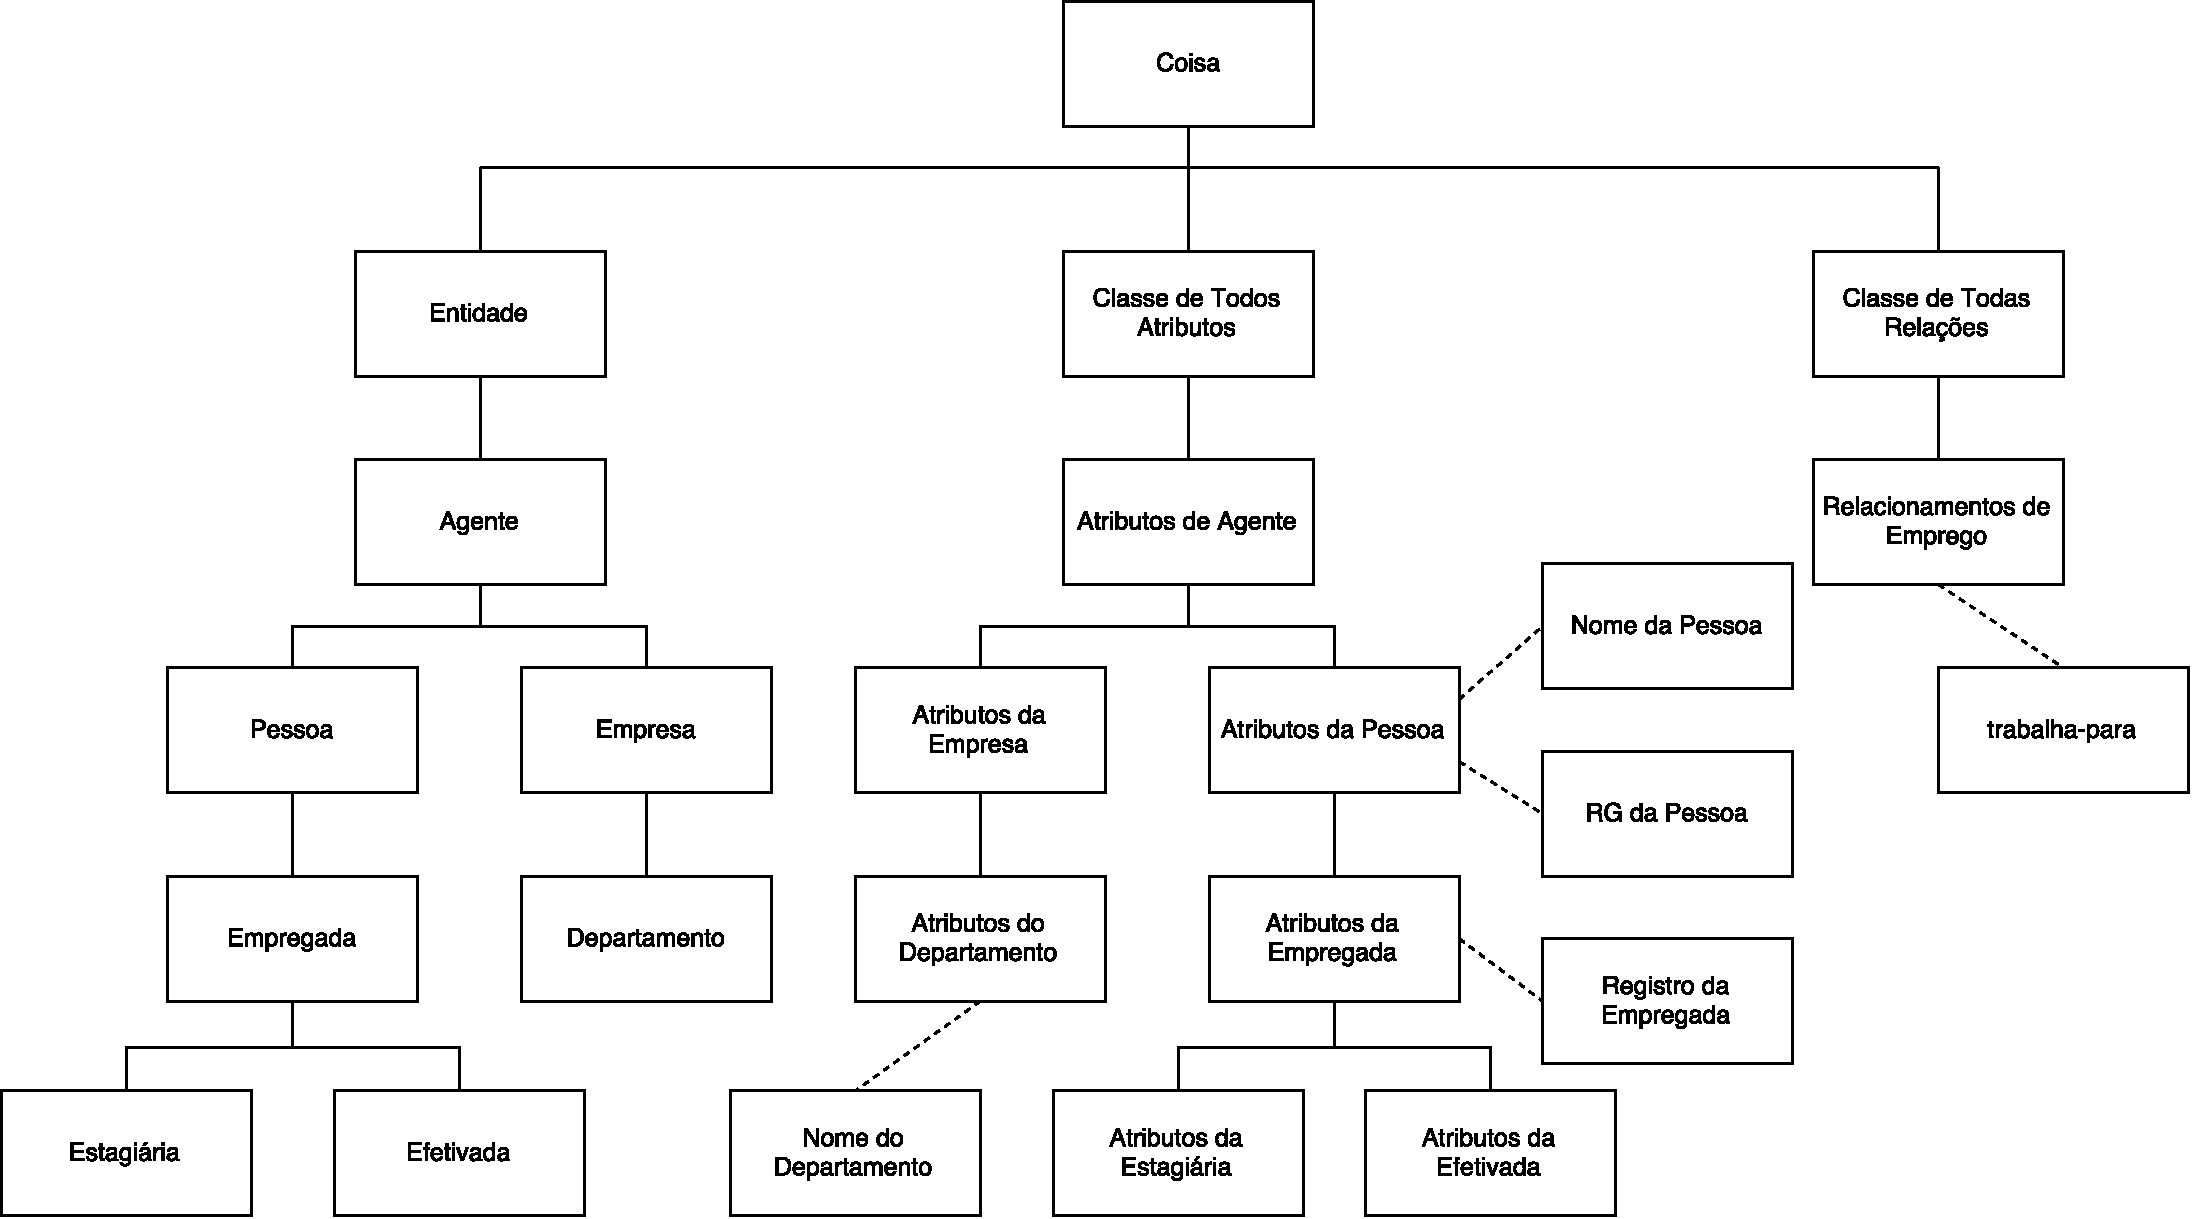
\includegraphics[width=1\textwidth]{pdf/ontology-weiss.pdf}
\end{figure}

Apesar de muito utilizada na área de IA, o uso de ontologias se tornou comum na Internet, possibilitando diversas categorizações em sites de acordo com os conteúdos neles apresentados \cite{NOY2001}. Esta prática facilita a busca de informações realizada por agentes eletrônicos, bem como a integração de gerenciamento do conhecimento e processos comerciais. A partir do uso de ontologias, a estruturação das informações e seu acesso nas redes de computadores tornou-se mais fácil \cite{MAEDCHE2002}.

Uma ontologia não é, simplesmente, uma taxonomia de classes ou tipos: nela, os relacionamentos entre as classes também devem ser descritos, mas suas instâncias não precisam ser representadas.  Ou seja, a ontologia é análoga a um esquema de banco de dados e não ao conteúdo do banco de dados em si \cite{WEISS1999}. Os conceitos ontológicos podem ser representados através de lógica de primeira ordem \cite{WEISS1999}, porém também é comum o uso de linguagem natural para a especificação \cite{UFG2007}. Um exemplo de especificação de definição em lógica de primeira ordem é dado na Expressão Lógica \ref{el:logica-1-ordem}.

\lstset{
    captionpos=b,
    caption={Exemplo de conceitos representados em lógica de primeira ordem onde a última sentença apresenta uma regra que expressa a noção de um tipo de hierarquia \cite{WEISS1999}},
    escapechar=1,
    basicstyle=\ttfamily
}

\vspace{0.4cm}
\begin{lstlisting}[label={el:logica-1-ordem},frame=single]
1$\forall{x}$1 (Bloco x) 1$\Rightarrow$1 (ObjetoFisico x)
(classe Bloco)
(classe ObjetoFisico)
(subclasseDe Bloco ObjetoFisico)
1$\forall{x, y, z}$1 (InstanciaDe x y) 1$\land$1 (SubclasseDe y z) 1$\Rightarrow$1 (InstanciaDe x z)
\end{lstlisting}


Segundo \cite{UFG2007},  a ontologia,  de acordo com o seu grau de formalismo, será categorizada em uma das quatro categorias abaixo:
\begin{description}
    \item [Altamente informais] são assim categorizadas quando expressas em linguagem natural;
    \item [Semi-informais] também expressas em linguagem natural, entretanto de forma estruturada;
    \item [Semi-formais] ontologias expressas em linguagem artificial definida formalmente;
    \item [Rigorosamente formais] são categorizadas desta forma quando seus termos são definidos a partir de uma semântica formal, teoremas e provas.
\end{description}

Neste trabalho, a ontologia pertence, de acordo com o seu grau de formalismo, à esfera formal. Por outro lado, em relação à sua função, classifica-se no âmbito das ontologias de domínio, isto é, ontologias que: 
\begin{directcite}
    descrevem conceitos e vocabulários relacionados a domínios particulares, tais como medicina ou computação, por exemplo.  Este é o tipo de ontologia mais comum, geralmente construída para representar um “micromundo” \cite{UFG2007}.
\end{directcite}Esta ontologia será abordada como forma de gestão do conhecimento, todavia, em outros contextos,  sua utilização pode apresentar diversos propósitos,  como o auxílio em processamento de linguagem natural, em web-semântica e na educação em ambientes online \cite{UFG2007}.

\subsection{Criando uma Ontologia}
Segundo o guia desenvolvido por \cite{NOY2001}, o primeiro passo a ser seguido é a escolha do domínio e escopo da ontologia. Antes de começar a criá-la, deve-se ter em mente que há diversas ontologias já desenvolvidas, as quais se encontram disponíveis na Internet. Para poupar tempo e retrabalho, uma boa prática é realizar uma pesquisa para descobrir se já não existem trabalhos similares ao que se deseja criar. Sendo assim, é possível acessar bibliotecas de ontologia desenvolvidas para serem reutilizadas, como a Protege Ontology Library\footnote{https://protegewiki.stanford.edu/wiki/Protege\_Ontology\_Library}, e também ter uma ideia de como desenvolver sua própria ontologia.

Para o segundo passo, sugere-se listar os termos considerados importantes neste domínio. Usando como exemplo o tema desenvolvido neste trabalho -- o de um cardápio para restaurantes e estabelecimentos semelhantes -- alguns dos termos que poderiam ser destacados são: \emph{comida} e \emph{bebida}, palavras que representam os tipos de produtos oferecidos no local; \emph{pastel} e \emph{torrada}, para os tipos específicos de lanches; \emph{quantidade}, \emph{ingrediente} e \emph{preço}, para características específicas de cada item do cardápio. A partir desta seleção, torna-se possível a definição das classes e das hierarquias de classes da ontologia que está sendo desenvolvida. Para isso, pode-se começar este desenvolvimento de três formas:
\begin{description}
    \item [De cima para baixo (\emph{top-down})] aqui, define-se os conceitos mais gerais e abrangentes primeiro e, então, os termos mais específicos. Para este trabalho, por exemplo, seria possível começar com termos como \emph{Comida} e, a partir disso, especializar esta classe com subclasses, como \emph{Pastel}, e assim em diante, criando as classes de \emph{Pastel de Carne}, \emph{Pastel de Quatro Queijos}, etc.
    \item [De baixo para cima (\emph{bottom-up})] este processo começa com a definição de termos específicos e, em seguida, com o agrupamento destes termos em classes mais amplas.
    \item [Combinação (\emph{combination})] técnica que consiste na combinação dos dois métodos citados anteriormente. Os termos são definidos sem uma ordem específica e depois são conectados com as classes mais (ou menos) genéricas. Normalmente, é vista como a abordagem mais fácil entre os desenvolvedores de ontologias (Rosch\footnote{Rosch, E., 1978, Principles of Categorization. Em R. E. e B. B. Lloyd, eds. \emph{Cognition and Categorization} pp. 27-48. Lawrence Erlbaum Publishers, Hillside, NJ.} , 1978 citado por \cite{NOY2001}).
\end{description}

A Figura \ref{fig:nivel-ontologia} ilustra os diferentes níveis presentes em uma ontologia:

\begin{figure}[H]
	\centering
	\caption[Níveis da Ontologia]{\label{fig:nivel-ontologia}Diferentes níveis da ontologia de uma lancheria}
    \begin{tikzpicture}
        \node (fig1) at (0,0){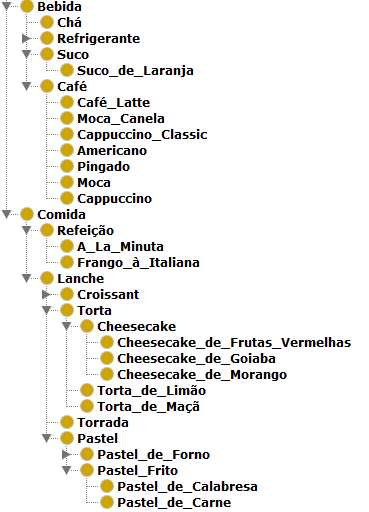
\includegraphics[scale=1]{fig/protege1.png}};
        \node (superior) at (4.5,6.2) {Nível superior};
        \node (intermediario) at (4.5,1.8) {Nível intermediário};
        \node (inferior) at  (4.5,-4.9) {Nível inferior};
        % -------------------------------------- 
        \node (bebida) at (-2,6.6) {}; % superior
        \node (cha) at (-2,6.2) {}; % superior
        \node (refrigerante) at (-0.6,5.8) {}; %superior
        \node (pingado) at (-1,2.3) {}; % intermediario
        \node (moca) at (-1.2,1.9) {}; % intermediario
        \node (cappuccino) at (-0.4,1.5) {}; % intermediario
        \node (cheesecake-morango) at (2.9,-3.4) {}; % inferior
        \node (pastel-calabresa) at (2.2,-5.9) {}; % inferior
        \node (pastel-carne) at (1.8,-6.6) {}; % inferior
        \draw[<-] (bebida) -- (superior);
        \draw[<-] (cha) -- (superior);
        \draw[<-] (refrigerante) -- (superior);
        \draw[<-] (moca) -- (intermediario);
        \draw[<-] (cappuccino) -- (intermediario);
        \draw[<-] (pingado) -- (intermediario);
        \draw[<-] (cheesecake-morango) -- (inferior);
        \draw[<-] (pastel-calabresa) -- (inferior);
        \draw[<-] (pastel-carne) -- (inferior);
    \end{tikzpicture}
\end{figure}

O terceiro passo é o de definição das propriedades das classes, responsável pela descrição de sua estrutura interna. Estas propriedades indicam quais são as características de cada item da classe, podendo ser propriedades intrínsecas, extrínsecas, partes que compõem esta classe ou a relação desta classe com um outro indivíduo. Subclasses herdam características das classes mais abrangentes; sendo assim, um campo específico deve pertencer à classe mais genérica da hierarquia que possui esta característica, uma vez que suas derivações terão, automaticamente, esta mesma estrutura. No exemplo trabalhado nesta seção, a classe \emph{Bebida} teria informações gerais como \emph{nome}, \emph{temperatura} e \emph{nível de açúcar} e todas suas subclasses herdariam estes atributos. As características das classes devem ser tipificadas de acordo com seu valor, podendo ser \emph{Strings}, números, \emph{booleanos}, instâncias, entre outros. No caso de campos caracterizados como instâncias, cria-se uma relação entre a classe que possui o campo (classe \emph{domínio}) e a instância da propriedade (classe de \emph{contradomínio}).

\section{Internet das Coisas}
Com o crescimento maciço de celulares e dispositivos \emph{tablets}, o uso de tecnologias sem fio tornou-se algo comum e fundamental na vida de diversas comunidades \cite{SHIN2014}. Recentemente, múltiplos aparelhos também começaram a se conectar à rede, como veículos, eletrodomésticos, aparelhos vestíveis e até postes de luz, introduzidos com o conceito de \emph{cidades inteligentes} -- cidades com uma infraestrutura monitorada e integrada através da Internet. A União Internacional de Telecomunicações (ITU) define a IoT como uma infraestrutura de rede global dinâmica com capacidades de auto-configuração baseadas em padrões e protocolos de comunicação interoperáveis, onde “coisas” possuem características próprias e estão integradas em uma rede de informações \cite{FRIESS2013}. \cite{FRIESS2013} ressalta que, apesar de recente, a IoT tem sido foco de organizações como Google, Apple e Cisco. Outras empresas, como a Huawei, vêm desenvolvendo projetos de cidades inteligentes em grandes cidades brasileiras; um exemplo disso é o \emph{Smart City Innovation Center}, localizado na Pontifícia Universidade Católica do Rio Grande do Sul, em Porto Alegre \cite{RIGON2016}.

\cite{FRIESS2013} destaca a notória intensificação do uso da Internet nos últimos anos. Em 2011, o número de dispositivos conectados à Internet ultrapassou o número de pessoas vivendo no planeta, e a estimativa é que, em 2020, o número de dispositivos esteja entre 26 bilhões e 50 bilhões. A previsão é que megacidades tornem-se inteligentes, entretanto ainda há programas pilotos sendo aplicados para tratar temas como segurança, aceitação por parte dos usuários e validação de ambientes inteligentes cooperativos. Por ser um sistema nupérrimo\footnote{Muito recente.}, \cite{SHIN2014} desenvolveu uma pesquisa buscando entender questões sociais e culturais relacionadas à IoT e concluiu que ainda há uma grande preocupação por parte da sociedade em relação à privacidade.

No momento, a IoT ainda é controversa e exige estudos e experimentos. Todavia, ao ser melhor desenvolvida e implantada em ambientes urbanos, pode ser integrada a diversos sistemas e auxiliar a população em suas tarefas cotidianas. O sistema proposto neste trabalho seria beneficiado através da conexão entre a aplicação móvel e um cardápio inteligente disponível em restaurantes. Este cardápio teria controle do número de instâncias de produtos disponíveis no local e enviaria estas informações à aplicação. Desta forma, seria apresentado ao usuário apenas os alimentos que estão, de fato, sendo vendidos no momento; prática que já é comum em lancherias que disponibilizam seus lanches em uma vitrine.


\section{Trabalhos Relacionados}
Algumas pesquisas foram realizadas com o intuito de conhecer ferramentas e obras similares a esta proposta. A busca foi realizada através de plataformas de pesquisa acadêmica como Google Scholar, ACM Digital Library e IEEE Xplore, além das lojas de aplicativos para Android, a Google Play, e iOS, a App Store; mesmo esta última não sendo o alvo de desenvolvimento desta aplicação, foi considerada importante a análise para conhecer os diversos aplicativos disponíveis no mercado e agregar valor ao trabalho. Foram encontrados alguns projetos que abordam o tema aqui proposto, além de trabalhos que tratam de temas similares. Ambos serão apresentados a seguir.

% \subsection{Trabalhos que Tratam de Acessibilidade}

\subsection{\label{subsec:zomato}Zomato}
Desenvolvido para iOS e previamente chamado de Urbanspoon\footnote{https://itunes.apple.com/br/app/urbanspoon-restaurant-food/id284708449?mt=8},  esta aplicação apresenta classificações e críticas sobre restaurantes com o intuito de ajudar o usuário a encontrar a melhor opção para sua refeição. Utilizando dispositivos com, por exemplo, Sistemas de Posicionamento Global (GPS -- \emph{Global Positioning Systems}), o Zomato\footnote{https://itunes.apple.com/br/app/zomato/id434613896?mt=8} detecta restaurantes nas proximidades e apresenta características como avaliações, cardápio e média de preço, permitindo, também, que a pessoa ordene as localidades por proximidade ou popularidade e salve seus locais favoritos. Ao ser realizado um teste com a aplicação, notou-se algumas falhas no seu desenvolvimento. Este não é um aplicativo criado para pessoas com deficiência visual, apenas oferecendo suporte completo para a ferramenta de leitura de tela da Apple, o VoiceOver\footnote{http://www.apple.com/br/accessibility/osx/voiceover/}. Por conta de não ter sido desenvolvido especialmente para usuários com deficiência visual, algumas telas podem apresentar dificuldades ao usuário, como mostrado na Figura ~\ref{fig:zomato1}(b), onde muitos itens acabam sendo sobrepostos.

\begin{figure}[H]
    \centering
    \caption[Ferramenta Zomato]{Telas do aplicativo Zomato}
    \label{fig:zomato1}
    \subfigure[a][Tela inicial da aplicação]
        {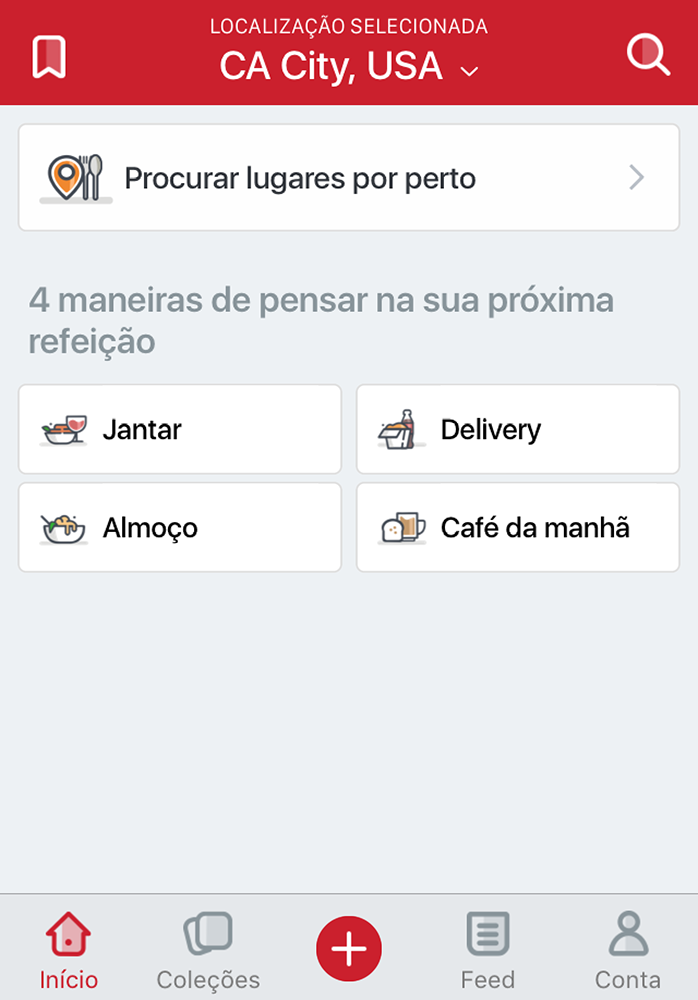
\includegraphics[width=0.27\textwidth]{fig/zomato1.PNG}}
        \qquad
    \subfigure[b][Visualização dos restaurantes no mapa]
        {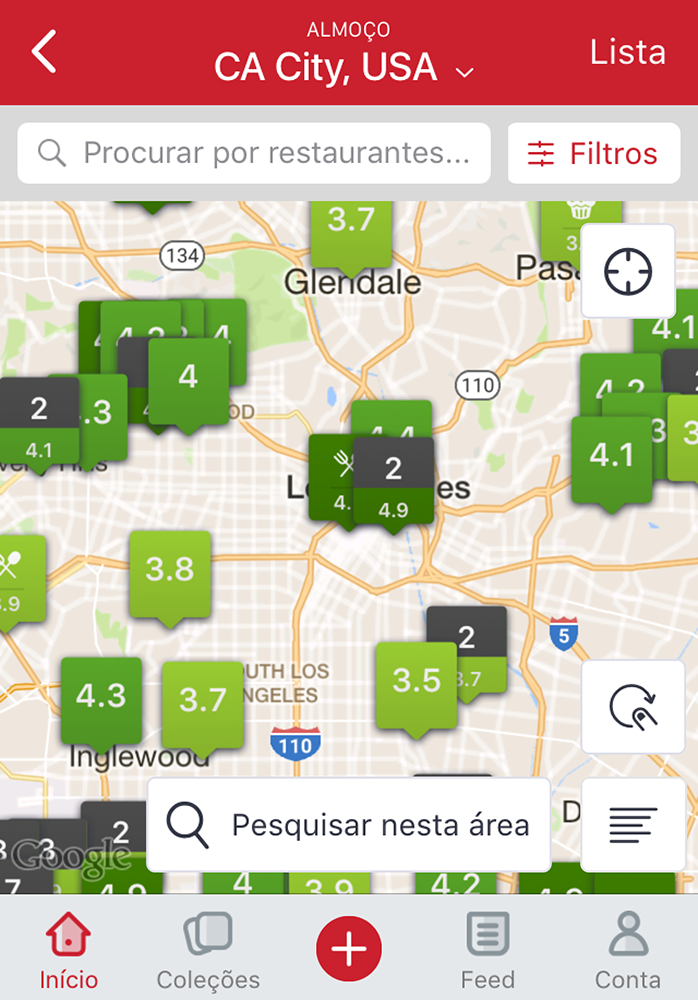
\includegraphics[width=0.27\textwidth]{fig/zomato4.PNG}}
        \qquad
    \subfigure[c][Opção para filtrar resultados]
        {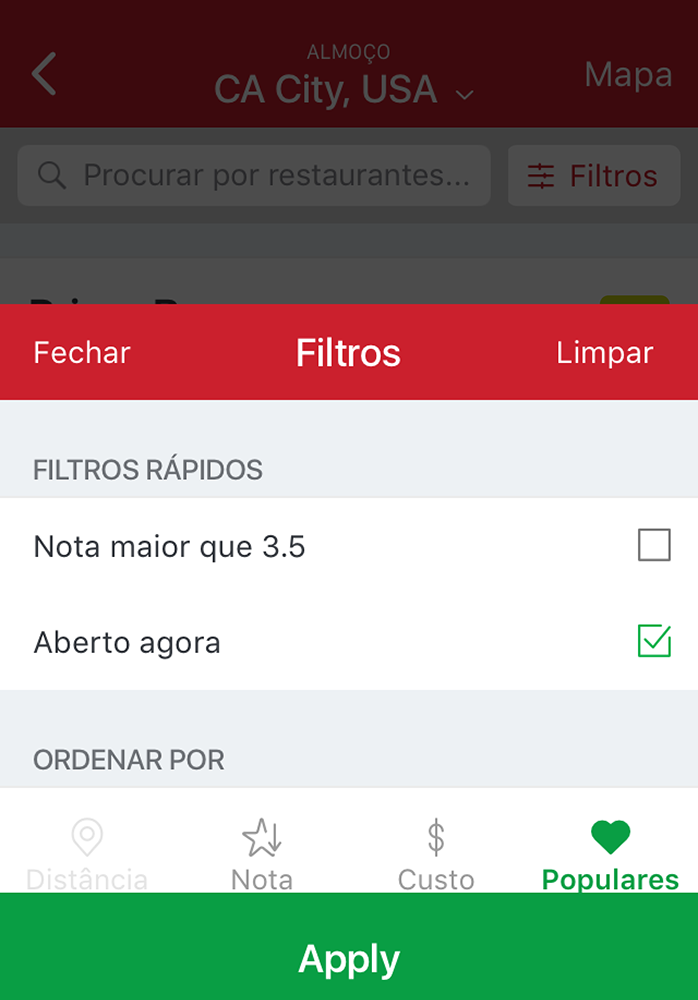
\includegraphics[width=0.27\textwidth]{fig/zomato3.PNG}}
\end{figure}

\subsection{Kapten PLUS}
Um dispositivo de locomoção disponível no mercado é o Kapten PLUS -- Dispositivo de Navegação Pessoal (Figura \ref{fig:fig2}). Através de um GPS, o sistema indica, proferindo comandos, onde o usuário está localizado e quais passos deve seguir para chegar em seu destino. O sistema também é composto por um controle, o qual possui uma interface tátil com botões em alto relevo. Este controle é necessário para que a pessoa possa inserir comandos e navegar pelos menus do sistema. Apesar de compacto, a utilização do sistema pode ser cansativa, uma vez que o usuário deve realizar a inserção de texto através de setas (para cima, para baixo, para esquerda e para direita) e também deve confirmar cada letra ou comando escolhido \cite{KAPTEN}.

\begin{figure}[H]
\centering
\caption[Ferramenta Kapten PLUS]{\label{fig:fig2}Kapten PLUS (Denham, 2011)}
\includegraphics[width=.70\textwidth]{fig/kapten1.jpeg}
\end{figure}

%\subsection{Trabalhos que Conjugam Inteligência Artificial e Acessibilidade a Pessoas com Deficiência Visual}

\subsection{Um Assistente Inteligente para Navegação de Pessoas com Deficiência Visual}
Já no ano de 2001, projetos para o auxílio de pessoas com deficiência visual eram desenvolvidos. Com o intuito de guiar seus usuários pela cidade, o artigo apresenta um sistema que utiliza diversos aparatos anexados ao corpo da pessoa que, juntos, servem como um guia para sua locomoção. Através de um GPS, uma câmera, sinais de áudio e diversos outros artefatos, a aplicação obtém informações sobre o local onde o usuário se encontra e os objetos a sua volta e, com isso, envia-lhe sinais de áudio para que ele possa transitar pela cidade. Esta interação é feita através de um agente incorporado no sistema e é este agente que irá se comunicar com o usuário e indicar-lhe as melhores rotas.

Com a utilização de um agente inteligente, as interações humano-agente se dão através de perguntas feitas pelo usuário que serão respondidas pela máquina, onde as informações fornecidas são calculadas através dos equipamentos embutidos no sistema. A implementação do sistema combina metodologias de IA, como interpretação de imagens, voz, linguagem natural, interpretação de conhecimento e conversação \cite{BOURBAKIS2001}.

\subsection{Um Sistema Robótico para a Localização de Pessoas com Deficiência Visual}
Há locais como aeroportos, centros de conferência e outros ambientes desconhecidos onde cães guias, bengalas e demais equipamentos acabam limitando a pessoa que é cega, não oferecendo o auxílio completo que elas possam necessitar. Em contrapartida, o uso de robôs nestas localidades traz diversas vantagens para o cidadão, uma vez que estes agentes podem traçar caminhos que levem o acompanhante a um ponto desejado, como um portão de embarque ou ao elevador mais próximo.

O agente comunica-se através de comandos reproduzidos em áudio, cuja maioria foi entendida pelos usuários que participaram dos testes. Todavia o reconhecimento dos comandos pela parte do agente não apresentou bons resultados, uma vez que os sistemas de reconhecimento de voz ainda estão em desenvolvimento. Outro problema apresentado pelo sistema é em relação à comunicação entre o usuário e outras pessoas que se encontram no ambiente. Por estar sempre ativo, aguardando comandos, o agente acabava por se confundir ao tentar interpretar o que estava sendo dito \cite{KULYUKIN2002}. 

\subsection{AudioGuider}
AudioGuider -- Sistema Eletrônico para Auxílio em Viagens Baseado em Comandos de Áudio é outra ferramenta que auxilia pessoas com deficiências visuais através do uso de GPS e câmera, com a premissa de ser barato e fácil de carregar. Como outros Sistemas Eletrônicos de Auxílio em Viagens (ETA -- \emph{Electronic Travel Aid Systems}), este dispositivo busca auxiliar os usuários em locais desconhecidos através da captura de imagens e localização do usuário. Além disso, este sistema também faz uso de áudio para indicar a distância entre a pessoa e objetos ou a pessoa e seu destino de chegada, utilizando fatores como volume, frequência e ritmo. Por exemplo: ao indicar um destino, o sistema começa a tocar uma determinada música. No momento em que o usuário estiver a cem metros do local, um som de bipe é emitido e a música começa a diminuir até ele chegar ao seu destino \cite{ZHIGANG2010}.

\subsection{Good Food Talks}
Desenvolvido para auxiliar a população com deficiência visual do Reino Unido, Good Food Talks\footnote{http://goodfoodtalks.com/} é um site que disponibiliza o cardápio de diversos restaurantes de forma acessível, tendo como suporte os aplicativos de acessibilidade do sistemas operacionais iOS\footnote{http://www.apple.com/br/accessibility/ios/voiceover/} e Android\footnote{https://play.google.com/store/apps/details?id=com.google.android.marvin.talkback\&hl=pt\_BR}. Na página inicial, o usuário depara-se com as opções de encontrar restaurantes em sua proximidade ou acessar a lista de restaurantes, além de poder inserir o nome de um restaurante específico. Ao selecionar o local desejado, o cardápio é apresentado na tela, trazendo o nome do item, uma descrição e seu preço. O site também oferece instruções de rota de acordo com a localização da pessoa. Entretanto, para um restaurante se cadastrar no sistema, é necessário pagar uma taxa anual de £199. Além disso, ao acessar a aplicação, foi constatado que, como visto na Figura ~\ref{fig:gft1}(a), a interface nem sempre respeita os princípios citados na seção \ref{sec:acessibilidade}.

\begin{figure}[htb]
    \centering
    \caption[Ferramenta Good Food Talks]{Telas do site Good Food Talks}
    \label{fig:gft1}
    \subfigure[c][Tela inicial da aplicação, onde o menu acaba empurrando o conteúdo principal para baixo]
        {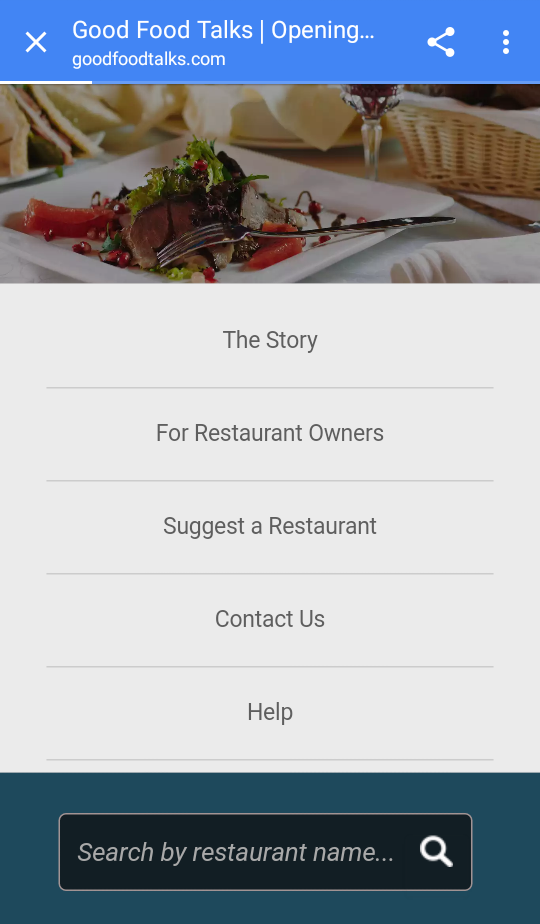
\includegraphics[width=0.27\textwidth]{fig/gft1.png}}
        \qquad
    \subfigure[c][Lista de restaurantes]
        {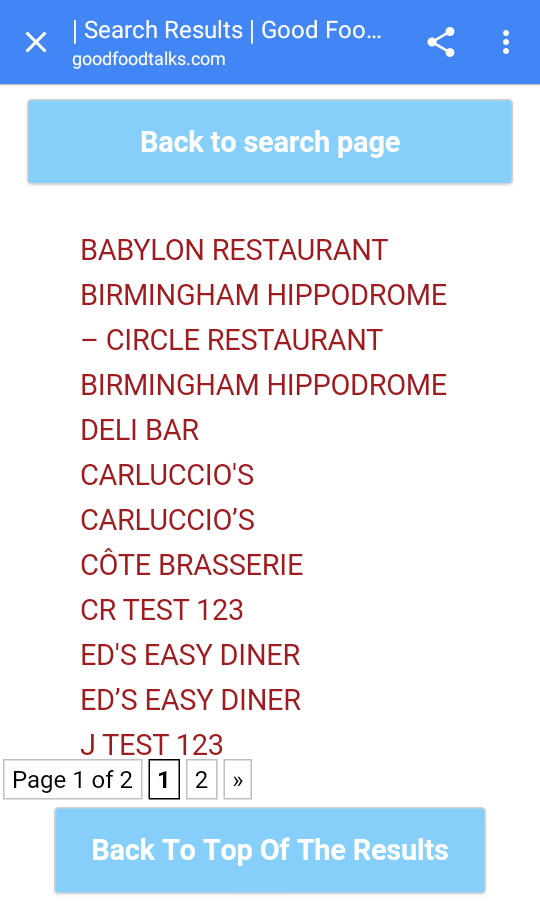
\includegraphics[width=0.27\textwidth]{fig/gft3.png}}
        \qquad
    \subfigure[c][Seção de vinhos do cardápio de um restaurante]
        {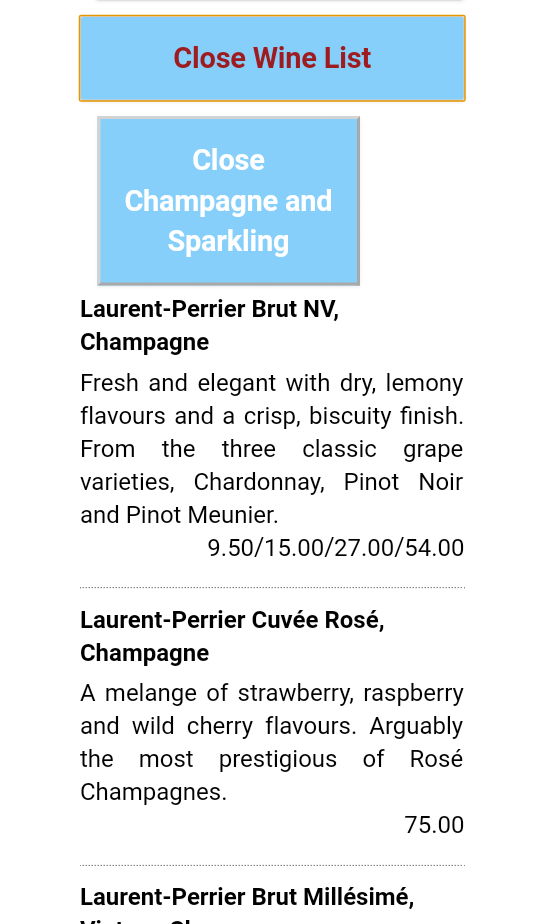
\includegraphics[width=0.27\textwidth]{fig/gft5.png}}
\end{figure}

\subsection{\label{subsec:tappy}Tappy Menu}
Tappy Menu\footnote{https://play.google.com/store/apps/details?id=com.ideal.tappymenu} é um aplicativo criado para dar mais liberdade a pessoas com deficiência visual que buscam acessar menus de restaurantes. De acordo com a descrição do Tappy Menu disponível na Google Play Store\footnote{https://play.google.com/store}, considerou-se necessária a criação desta aplicação, uma vez que as opções de cardápios em braile, fornecidas pelos estabelecimentos, tendem a estar desatualizadas. Ademais, uma parcela de pessoas com deficiência visual não possui domínio sobre a linguagem braile, reforçando a necessidade de tal aplicação. Tappy indica ser uma ferramenta completa para seus usuários, oferecendo cardápios detalhados, com informações nutricionais, ingredientes, preços, entre outros. Todavia, ao instalar e navegar pela aplicação, foi percebida a presença de alimentos que possuem informações parciais (Figura ~\ref{fig:tappy1}(a)) ou informações espalhadas pelas seções do aplicativo (Figuras ~\ref{fig:tappy1}(b) e ~\ref{fig:tappy1}(c)). Desenvolvido nos Estados Unidos, a aplicação dá suporte a onze restaurantes da região.

\begin{figure}[htb]
    \centering
    \caption[Ferramenta Tappy Menu]{Telas do aplicativo Tappy Menu}
    \label{fig:tappy1}
    \subfigure[c][Tela de ingredientes de um dos produtos do cardápio da sorveteria Carvel]
        {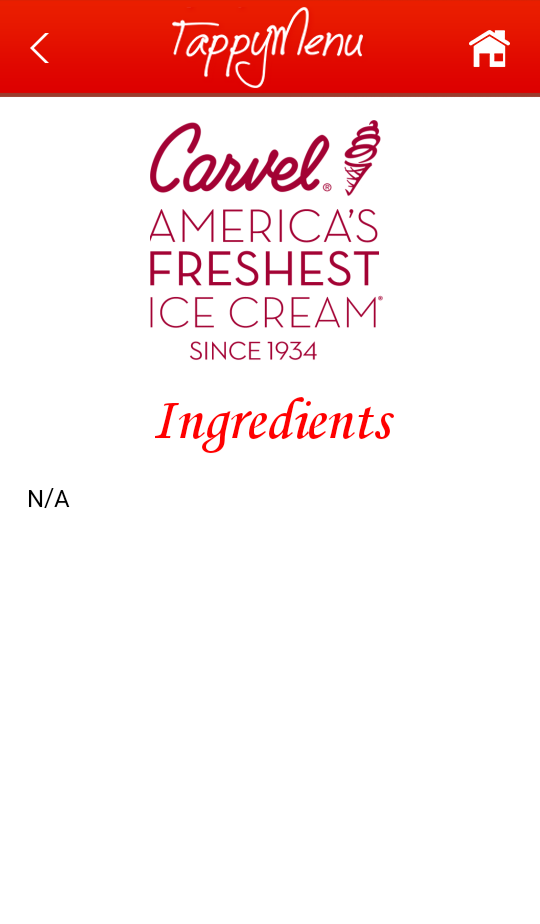
\includegraphics[width=0.27\textwidth]{fig/tappy3.png}}
        \qquad
    \subfigure[c][Descrição das refeições já apresenta os ingredientes para o usuário]
        {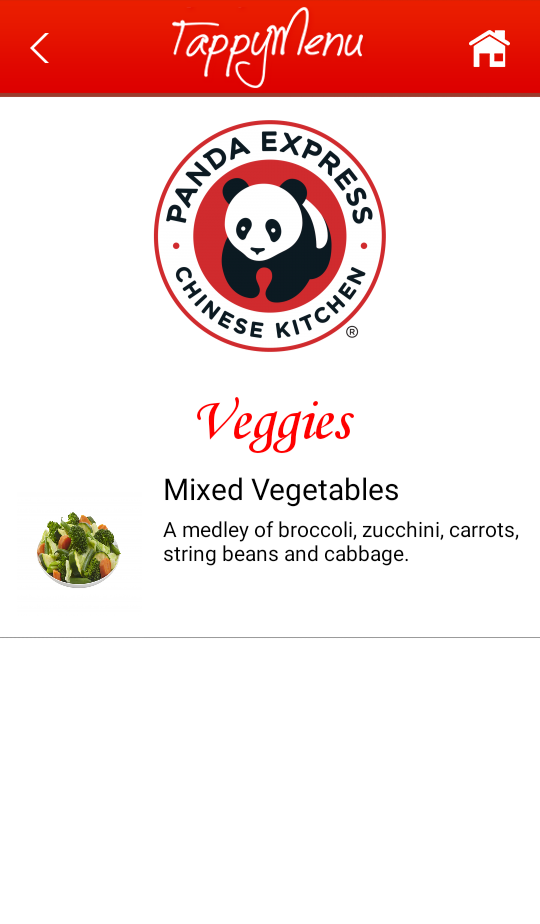
\includegraphics[width=0.27\textwidth]{fig/tappy4.png}}
        \qquad
    \subfigure[c][Tela de ingredientes da opção previamente selecionada, exibindo apenas os ingredientes que causam alergia]
        {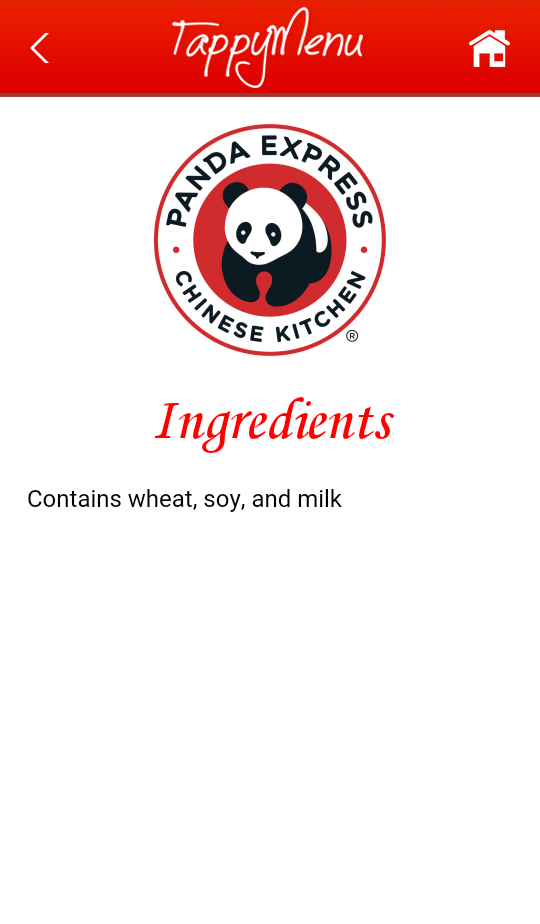
\includegraphics[width=0.27\textwidth]{fig/tappy2.png}}
\end{figure}

\section{Visão Geral das Aplicações}

Os aplicativos para dispositivos móveis testados e apresentados nesta seção (\ref{subsec:zomato} e \ref{subsec:tappy}) apresentaram alguns descuidos ao almejar fornecer uma aplicação acessível e fluída aos seus usuários. Ao serem testadas com as ferramentas VoiceOver e TalkBack (respectivamente), evidenciou-se que algumas melhorias ainda precisavam ser feitas, como citado anteriormente nas seções correspondentes a tais aplicações. Além disso, o fluxo da aplicação Tappy Menu não está conciso e pode confundir o usuário. Os demais sistemas não puderam ser testados com ferramentas similares pela restrição de acesso ou falta de softwares que exercem tal função, entretanto a familiarização com os projetos puderam trazer um conhecimento básico sobre o que eles fornecem e como lidam com questões voltadas à acessibilidade. Sendo assim, através da análise feita com este conjunto de aplicações, observou-se artifícios e ideias que podem ser agregadas ao cardápio virtual, bem como práticas que deverão ser evitadas.
		\chapter{\label{chap:requi}Requisitos}
Nesta seção, serão apresentados os requisitos funcionais e não funcionais levantados durante o processo de modelagem de software.

\section{Requisitos Funcionais}
\begin{itemize}
    \item O sistema deve permitir que o usuário mantenha uma lista de locais favoritos;
    \item O sistema deve armazenar os itens do cardápio de acordo com a ontologia desenvolvida para restaurantes;
    \item O sistema deve informar o número de instâncias dos itens apresentados no cardápio;
    \item O sistema deve permitir a filtragem do menu de acordo com determinadas restrições alimentares;
    \item Através da ferramenta de localização, o sistema deve apresentar a lista de restaurantes mais próximos, caso o local esteja registrado no aplicativo.
\end{itemize}

\section{Requisitos Não-Funcionais}
\begin{itemize}
    \item A aplicação deve ser desenvolvida na plataforma Android;
    \item A aplicação deve ser desenvolvida em Java, através do Ambiente de Desenvolvimento Integrado (IDE -- \emph{Integrated Development Environment}) Android Studio;
    \item A aplicação deve fazer uso das ferramentas de localização e TalkBack disponíveis em dispositivos Android;
    \item A aplicação deve utilizar um banco de dados SQLite para o armazenamento de dados;
    \item A aplicação deve seguir os princípios do \emph{World Wide Web Consortium} (W3C) no quesito de acessibilidade para usuários com deficiência visual;
    \item A aplicação deve seguir os princípios de ergonomia relacionados à interação humano-computador, sugeridos por \cite{ERGO2015};
    \item A aplicação deve se guiar pelos padrões de design para aplicativos móveis.
\end{itemize}
		\chapter{\label{chap:modelagem}Modelagem}
A diretriz do desenvolvimento deste trabalho seguirá algumas propostas da metodologia Kanban. Desenvolvido no final da década de 1940 pela Toyota, o método Kanban apresenta ferramentas que diminuem o trabalho em progresso (\textit{work in process}) e  auxiliam na administração de custos e na identificação de gargalos e outros impedimentos no fluxo do desenvolvimento do processo \cite{GROSS2003}. Um processo guiado por Kanban terá suas características, peculiaridades e riscos destacados, possibilitando ao time uma rápida percepção dos possíveis problemas e oportunidades que determinada atividade poderá apresentar.

Essa é "uma técnica que traduz em linhas, colunas e cartões coloridos o fluxo existente no processo de produção"\ \cite{AUDY2015}. Palavra do idioma japonês, \textit{kanban} significa "quadro"\ \cite{GROSS2003} e este é o seu componente essencial -- um quadro com diversas colunas onde cada uma delas representa o estado de algum processo do projeto, como ilustrado na Figura ~\ref{fig:kanban1}. Por ser uma ferramenta sucinta e visual, uma rápida visualização do painel de tarefas deve permitir que se obtenha conhecimento de aspectos como: informações básicas sobre o processo; o estágio de cada um deles e qual sua prioridade ou nível de dificuldade, os quais são usualmente indicados por cores diferentes (Audy, 2015). 

Todos estes aspectos devem ser previamente definidos pelo time durante o processo de projeção do \textit{kanban}. Cada projeto possuirá um \textit{kanban} específico de acordo com seu escopo e sua equipe, sendo delegadas funções para cada integrante do time. Outro fator que deve ser definido são os limitadores, os quais definirão algumas regras para o fluxo do desenvolvimento do processo, como o número máximo de tarefas na fila de testes, entre outros \cite{AUDY2015}. Assim, cada integrante do time é responsável por manter o ritmo do processo e evitar que tarefas acumulem.

\begin{figure}[htb]
\centering
\caption[\emph{Kanban}]{\label{fig:kanban1}\emph{Kanban} criado na ferramenta Trello}
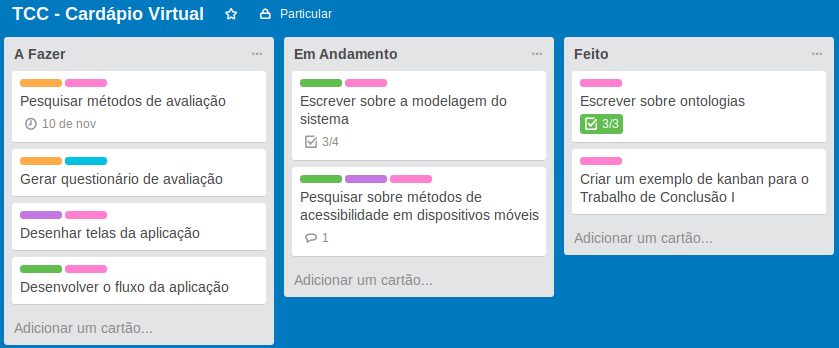
\includegraphics[width=0.8\textwidth]{fig/kanban1.png}
\end{figure}


\section{Planejamento}
Ao realizar o planejamento de um software, podem surgir alguns conflitos entre as diferentes partes interessadas. É possível que o cliente, o usuário, o desenvolvedor e outros integrantes do projeto tenham visões diferentes sobre o mesmo projeto e o resultado não venha a ser satisfatório para um dos lados \cite{COHN2004}. Neste caso, busca-se por uma forma em que todas as partes possam trabalhar juntas e entrar em um consenso e, para isso, é necessário que a equipe não aja de forma autocentrada e leve em consideração quem é seu usuário, o que ele quer e como ele se comporta \cite{AUDY2015}. Por isso, duas técnicas foram escolhidas para auxiliar no planejamento deste trabalho: o desenvolvimento de \textit{personas} e o uso de \textit{histórias de usuário}.


\section{Personas}

Conhecer e criar empatia com quem usufruirá do sistema são atividades necessárias, apesar de ainda pouco praticadas em algumas áreas do desenvolvimento de software. Uma forma de registrar informações acerca do cliente é a partir da criação de personas -- perfis fictícios de possíveis usuários do sistema a ser desenvolvido. Cada persona possui um nome, um perfil, um comportamento e um conjunto de necessidades que deseja suprir; sendo importante entender e traçar diferentes tipos de clientes, como um usuário comum e um usuário administrador, por exemplo \cite{AUDY2015}. Desta forma, esses perfis representarão uma parcela significativa dos clientes em potencial.

\cite{ERGO2015} destacam que
\begin{directcite}
    quando se pensa em análise para acessibilidade, o objetivo é conhecer os perfis dos futuros usuários de um sistema que são portadores de deficiência. (...) Assim, uma boa ideia é a elaboração de "personas"\ descrevendo o perfil de usuários portadores de deficiência e de "cenários problema"\ descrevendo as estratégias e o ambiente de trabalho atuais. 
    Essas personas e esses cenários seriam usados nas atividades de especificação e concepção da interface.
\end{directcite}
Tendo em vista a importância desta prática, as seções seguintes apresentarão três perfis de possíveis usuários do sistema a ser desenvolvido.

\subsection{Pessoa com Deficiência Visual em Busca de Restaurantes nas Proximidades}
Airy Gavião é estudante do curso de Sistemas de Informação em sua universidade. Com 22 anos, ela está no fim de sua graduação, mas, durante todos esses anos, Airy não possuía o costume de frequentar os bares e restaurantes das redondezas do prédio onde estudava, uma vez que não os considerava acessíveis para pessoas com deficiência visual. Normalmente, Airy trazia algum lanche que preparara em casa; evitava ter que comer em algum estabelecimento, uma vez que considerava ser um incômodo o ato de perguntar aos seus amigos quais eram as características das comidas apresentadas nos balcões das lancherias. 

Ao baixar o aplicativo de auxílio em restaurantes, Airy procurou pelos restaurantes e bares em sua proximidade, buscando por algum que possuísse registro no sistema. Os nomes dos restaurantes registrados foram listados ao usuário, o qual selecionou o primeiro da lista para conferir as informações básicas do local e seu cardápio. Por não comer carne, Airy deu preferência pelo acesso dos itens vegetarianos, apenas. Ao perceber que havia algumas opções que lhe agradavam, ela decidiu ir ao restaurante em questão.

Após sua refeição, levando em consideração a proximidade do local e o custo benefício, Airy decidiu adicionar o restaurante em sua lista de "locais favoritos". Para isso, Airy simplesmente acessou a tela de informações adicionais do restaurante e selecionou a opção de \emph{favoritar}.

\subsection{Pessoa com Deficiência Visual em Viagem}
Olinda Muniz é professora em uma pequena comunidade indígena no interior do estado e, apesar de possuir um celular, faz uso de apenas algumas aplicações. Com frequência, ela precisa viajar para outras regiões em congressos ou eventos educacionais e acaba pernoitando nessas cidades. Ao agendar uma viagem para Porto Alegre, a professora decide verificar os cardápios dos restaurantes próximos à Pontifícia Universidade Católica do Rio Grande do Sul, local onde será realizado o evento. Ao inserir o endereço da universidade, os  restaurantes são listados e ela pode acessar seus cardápios. Desta forma, Olinda pode sugerir o restaurante para seus amigos, uma vez que tem conhecimento do que é servido no local. 

\subsection{Alguém que Convive com Pessoas com Deficiências Visuais}
Vãngri Kaingáng, radialista de 30 anos, está em um relacionamento com uma pessoa com deficiência visual. Normalmente, quando decidem sair para jantar, Vãngri acaba lendo o cardápio físico para Rosane, mas percebe que ela não se sente muito a vontade e não faz muitas perguntas; ao encontrar uma opção que pareça agradável, Rosane a escolhe, sem checar outras opções.

Devido a este impasse, Vãngri pedia a seus ouvintes recomendações de restaurantes que fossem mais acessíveis ou sugestões de refeições de acordo com o gosto de Rosane. A partir disso, chegou ao conhecimento da aplicação móvel com cardápio acessível. Rosane acessou a aplicação e buscou pelo nome de restaurantes já conhecidos, analisando seus cardápios e marcando-os como favoritos. Com estas informações contidas na aplicação, Vãngri pode analisar as preferências de Rosane e, através do sistema de busca, encontrar novos restaurantes, cafés, bistrôs, entre outros.

\section{Histórias de Usuário}

Segundo \cite{COHN2004}, uma história de usuário (US -- \emph{User Story}) descreve uma funcionalidade que será valiosa para o usuário do software. Normalmente, segue a seguinte estrutura: \textit{"como um X, eu quero Y, porque Z"}; onde X é a pessoa beneficiada, Y é alguma funcionalidade do sistema e Z é o valor desta funcionalidade. Seguindo este modelo, cada história especifica quem é o usuário, qual sua necessidade e qual sua motivação \cite{AUDY2015}, podendo conter detalhes adicionais. Uma vez que as US são representações de funcionalidades que serão validadas pelo usuário, requisitos não-funcionais, como, por exemplo, a linguagem na qual o programa será desenvolvido, não são incorporados nelas \cite{COHN2004}. As histórias de usuário formuladas para este sistema serão apresentadas a seguir.

\subsection{US01 -- Acessar o sistema}

\textit{"Eu, como um usuário, desejo poder acessar o sistema quando achar necessário."}

Esta história de usuário apresenta a seguinte funcionalidade: a de aceso ao sistema. Com ela, o usuário é livre para entrar no sistema e ter acesso ao seu conteúdo, bem como sair dele. Para realizar tais tarefas, basta selecionar a aplicação e, ao carregá-la em seu dispositivo, informar seus dados de localização, os quais são obtidos através da conexão com o GPS.

\subsection{US02 -- Buscar Restaurante}

\textit{"Como usuário, desejo buscar restaurantes e acessar suas informações,  verificando quais restaurantes estão em minha proximidade e quais alimentos oferecem."}

A habilidade de buscar um restaurante no sistema e poder acessar suas informações é o que compõe esta história de usuário. O cliente deve ser capaz de buscar um restaurante no campo de busca através da inserção de texto ou por um comando de voz e, caso o restaurante esteja registrado no sistema, poderá selecioná-lo, sendo redirecionado à tela que contém as informações gerais do local. 

\subsection{US03 -- Acessar Cardápio}

\textit{"Como usuário, desejo acessar o cardápio dos restaurantes com o intuito de verificar as opções disponíveis e analisar as informações de cada alimento."}

O usuário deverá poder acessar os cardápios dos restaurantes registrados no sistema, bem como informações detalhadas das refeições. Estarão disponíveis os ingredientes de cada item do menu, além de informações adicionais que possam ser relevantes para os clientes.

\subsection{US04 -- Filtrar Cardápio}

\textit{"Eu, como usuário, busco poder filtrar as opções do cardápio de acordo com uma dieta específica, bem como outras categorias."}

O que caracteriza esta história de usuário é a possibilidade de filtrar cardápios de acordo com categorias pré-estabelecidas pelo sistema. Caso o usuário seja vegetariano, por exemplo, ele poderá selecionar a opção que apresenta apenas aqueles produtos que não contêm carne. Assim, a navegação no sistema será mais rápida e objetiva.

\subsection{US05 -- Favoritar Restaurante}

\textit{"Como um usuário, eu desejo poder favoritar certos locais, podendo ter fácil acesso a eles na aplicação."}

Nesta história, representamos a possibilidade de cada usuário ter uma lista pessoal de fácil acesso a locais de sua preferência. Podendo marcar um determinado local como "favorito", este estabelecimento ficará registrado em uma lista à parte, onde o usuário poderá acessá-la na página inicial do sistema. Sendo assim, caso deseje obter informações sobre o local, não será necessário procurar o restaurante no sistema de buscas.

\section{Fluxograma}
Um fluxograma é a representação visual da sequência de passos em um processo, onde diferentes passos são representados por caixas e o encadeamento destes passos é representado por setas \cite{REYNARD1995}. Estes diagramas ajudam a sistematizar um entendimento comum sobre o processo; a visualizar o processo como processos menores, os quais interagem entre si; a melhorar o processo, eliminando ineficiências; e a padronizar este processo, tornando-o mais consistente. Quando se deseja obter um esboço dos passos mais genéricos do processo em questão, \cite{REYNARD1995} indica o uso de um fluxograma básico sem atividades muito detalhadas. Um diagrama contendo estas características é apresentado a seguir, na Figura \ref{fig:fluxograma}.

\begin{figure}[H]
    \centering
    \caption[Fluxograma Geral do Sistema]{\label{fig:fluxograma}Fluxograma geral da aplicação. As setas tracejadas indicam a saída do sistema}
    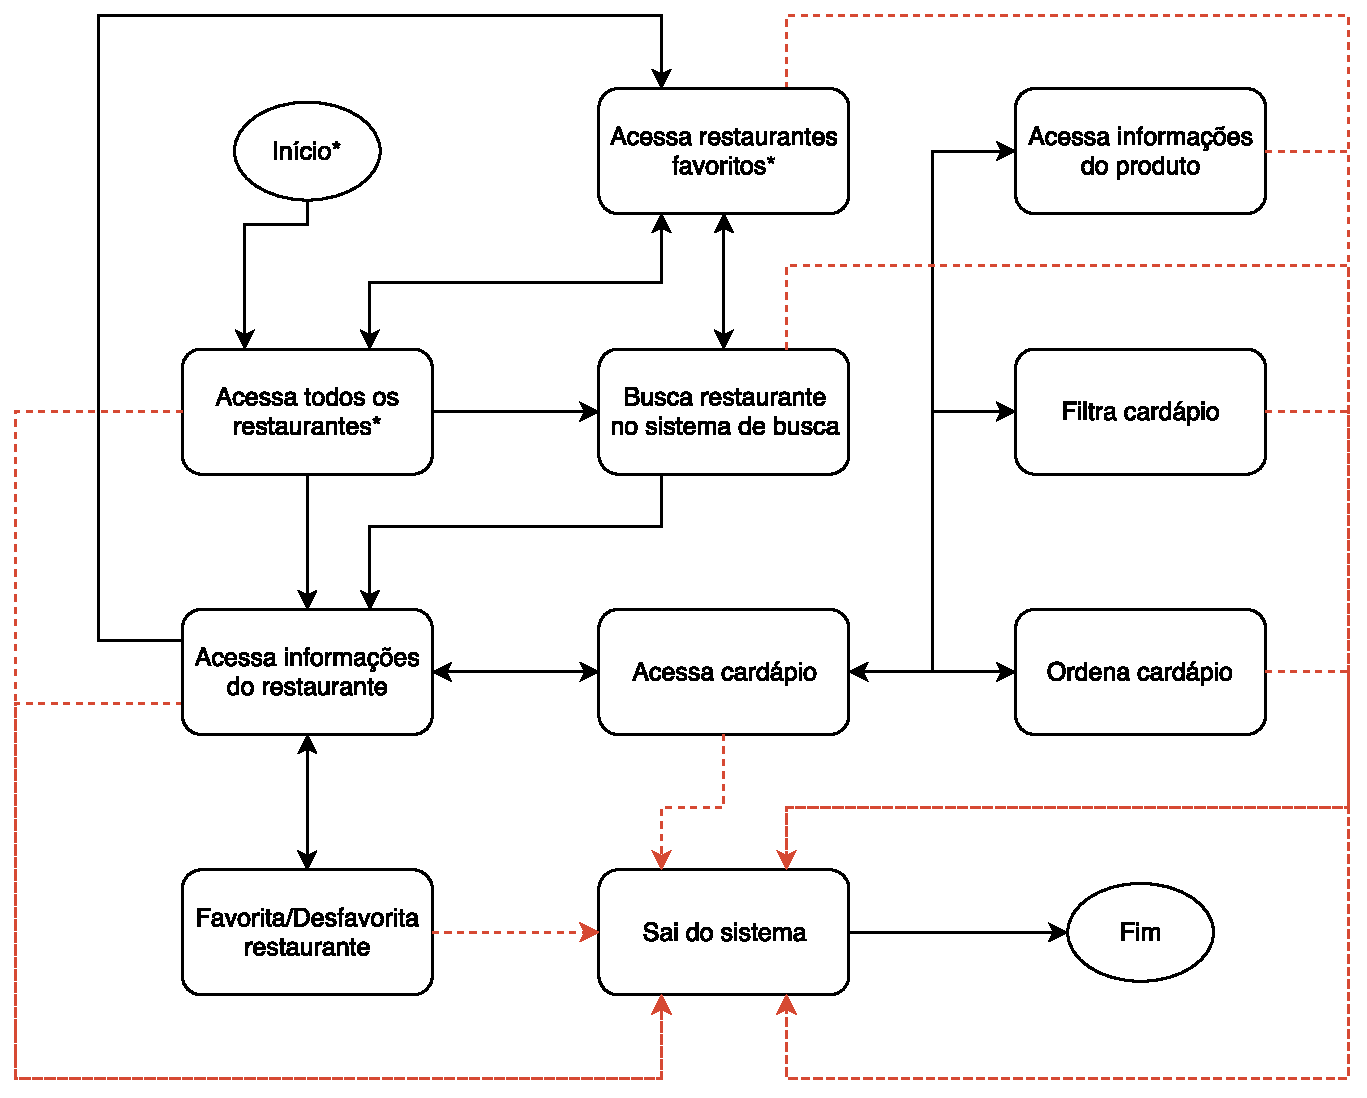
\includegraphics[width=0.9\textwidth]{./pdf/fluxograma-atual.pdf}
\end{figure}


\section{Modelagem do Banco de Dados}

A aplicação desenvolvida neste trabalho não requer uma estrutura de dados muito robusta. O banco de dados aqui desenvolvido é composto por quatro tabelas: \emph{Restaurantes, Logs, Categorias\_Produtos} e \emph{Dúvidas}. A tabela de Restaurantes é composta pelos dados básicos de cada localização, bem como suas coordenadas; além disso, também há uma coluna (\emph{Favorito}) que demarca se este restaurante fora marcado como favorito ou não pelo usuário. A tabela de Logs guarda o nome dos produtos e quantas vezes eles foram acessados -- este item será importante para um dos critérios de ordenação do cardápio. Já a tabela Categorias\_Produtos armazena a relação entre os produtos e a categoria a qual eles pertencem, auxliando na construção do cardápio. Por fim, a tabela de Dúvidas é uma estrutura criada para armazenar os dados referentes ao sistema de Ajuda da aplicação. As tabelas descritas previamente e suas relações podem ser vistas na Figura \ref{fig:bd}:

\begin{figure}[H]
	\centering
	\caption[Modelagem do Banco de Dados]{\label{fig:bd}Modelo do banco de dados para o sistema de Cardápios Virtuais}
	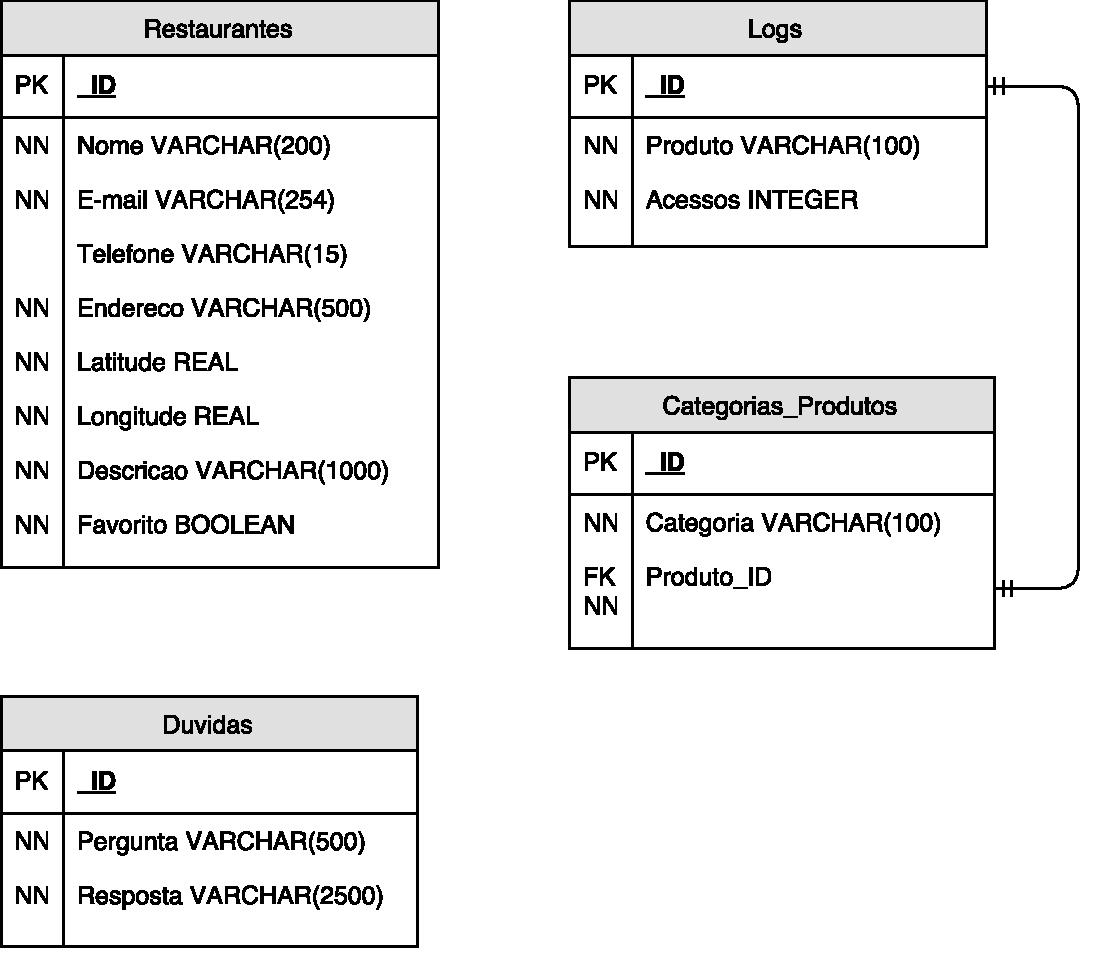
\includegraphics[width=0.9\textwidth]{./pdf/bd.pdf}
\end{figure}

\section{Estrutura das Classes}

		\chapter{\label{chap:recurs}Recursos Necessários}
Para tornar possível o desenvolvimento da aplicação proposta neste trabalho, é proposto o uso dos seguintes sistemas:
\begin{itemize}
    \item Java Platform, Standard Edition Development Kit (JDK) versão 8\footnote{http://www.oracle.com/technetwork/pt/java/javase/downloads/jdk8-downloads-2133151.html}, o qual oferece um conjunto de ferramentas para o desenvolvimento e teste de programas escritos na linguagem de programação Java;
    \item Android Software Development Kit (Android SDK);
    \item Android Studio\footnote{https://developer.android.com/studio/index.html}, IDE oficial para criação de aplicativos em dispositivos Android;
    \item SQLite\footnote{https://www.sqlite.org/}, banco de dados que armazenará os dados necessários para o funcionamento do aplicativo;
    \item Ferramenta Protégé\footnote{http://protege.stanford.edu/}, criada pela universidade de Stansford com o intuito de desenvolver ontologias; e
    \item Trello\footnote{https://trello.com/}, sistema de quadros onde o \emph{kanban} será desenvolvido.
\end{itemize}
Além desses recursos de software, há elementos de hardware cruciais para a criação desta aplicação:
    \begin{itemize}
        \item Um computador com, no mínimo, 2 GB de RAM e 5 GB de memória não-volátil; e
        \item Um dispositivo móvel com sistema operacional Android.
    \end{itemize}
		\chapter{\label{chap:desenvolvimento}Desenvolvimento}

O desenvolvimento do sistema pode ser dividido em duas partes: i) o desenvolvimento da ontologia de cardápio e ii) o desenvolvimento da aplicação móvel para Android. Primeiramente, foi desenvolvida a estrutura da ontologia para, posteriormente, integrá-la à aplicação. A seguir, será apresentado o desenvolvimento de ambas as partes do sistema, bem como as modificações realizadas a partir da proposta inicial da aplicação e as dificuldades encontradas durante a evolução do projeto.

\section{\label{sec:ontologia}Ontologia de Cardápio}

Apesar de haver algumas ontologias de comida ou restaurantes já desenvolvidas, optou-se pela criação de uma ontologia própria que condizesse com o escopo do trabalho. Para a construção desta ontologia para cardápios, foram usadas como base outras ontologias relacionadas a comidas. A principal influência foi uma ontologia de pizza desenvolvida pela universidade de Stanford\footnote{http://protege.stanford.edu/ontologies/pizza/pizza.owl}, uma vez que um cardápio é composto por diversos produtos que apresentam atributos semelhantes ao de uma pizza. Voltaremos a falar desses atributos nos próximos parágrafos.

A estrutura da ontologia é dividida em duas partições iniciais: \emph{Partição Domínio} e \emph{Partição Valor}. Dentro da partição de domínio, encontram-se os \emph{produtos} e os \emph{ingredientes}, os quais serão atribuídos aos produtos do cardápio. Os produtos da aplicação referem-se aos produtos do cardápio em si e é dentro desta classe que as informações essenciais a nossa aplicação estão armazenadas. Cada produto apresenta ou herda as seguintes propriedades:
\begin{itemize}
	\item Ingredientes;
	\item Preço;
	\item Restrições alimentares:
	\begin{itemize}
		\item Se possui glúten;
		\item Se possui lactose;
		\item Se é vegetariano;
		\item Nível de sal;
		\item Nível de gordura;
	\end{itemize}
	\item Se é um produto contável ou não.
\end{itemize}

Já a partição de valor é composta pelas classes \emph{Gorduras} e \emph{Nível de Sal}, representando todas as propriedades que podem ser compostas por uma gradação de valores. Cada uma dessas classes apresentam, por sua vez, três subclasses que condizem à intensidade destas propriedades em um produto. Desta forma, o nível de sal de uma determinada comida pode ser indicado com um dos três níveis criados na ontologia, sendo eles: \emph{pouco salgado}, \emph{meio salgado} e \emph{salgado}. Para a indicação desta propriedade no produto, criou-se a propriedade \emph{temSal} cujo domínio é uma classe do tipo Produto e o alcance é uma classe do tipo Nível de Sal. 

Para gerar relações entre classes e propriedades, foram criadas \emph{propriedades de objeto} e \emph{propriedades de dados}. As propriedades de objeto são utilizadas quando tanto o domínio quanto o alcance da expressão são classes da ontologia; já as propriedades de dados aplicam-se quando o alcance é composto por um tipo de dado, como um \emph{value} ou um \emph{boolean}. Algumas propriedades e suas relações com as classes são demonstradas a seguir, na Figura \ref{fig:propriedades}.
\begin{figure}
	\centering
	\caption[Propriedades da Ontologia]{Exemplos de propriedades da ontologia}
	\label{fig:propriedades}
	\subfigure[c][Propriedade \emph{temIngrediente}. Seu domínio são as classes \emph{Comida} ou \emph{Bebida} e o alcance, \emph{Ingrediente}]
	{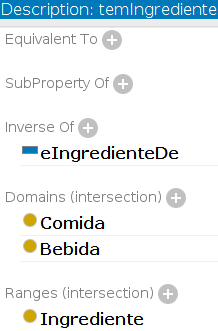
\includegraphics[width=0.3\textwidth]{./fig/propriedade-1.png}}
	\qquad
	\subfigure[c][Propriedade \emph{preco}. Seu domínio é a classe \emph{Produto} e o alcance, um valor do tipo \emph{double}]
	{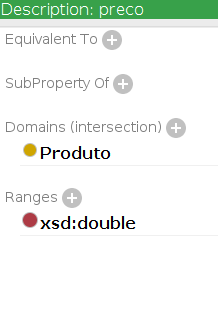
\includegraphics[width=0.3\textwidth]{./fig/propriedade-2.png}}
\end{figure}

\section{Integração da Ontologia com a Aplicação}

Sendo Java a linguagem de programação utilizada no desenvolvimento da aplicação, buscou-se uma API que fosse compatível com a linguagem e que consultasse a ontologia de forma eficiente. A princípio, a interface escolhida fora a OWL API\footnote{http://owlapi.sourceforge.net/}, uma interface para criação, manipulação e serialização de ontologias OWL. Todavia, apesar de ser desenvolvida para a linguagem Java, essa API não se apresentou compatível com o ambiente Android, sendo assim necessária uma nova busca, resultando na descoberta do \emph{framework} Apache Jena\footnote{https://jena.apache.org/}. Jena é uma ferramenta para a construção de aplicações que utilizam web semântica ou dados conectados (\emph{linked data}) e é responsável pelo controle de APIs de diversas estruturas de dados, como ontologias, Resource Description Framework (RDF), SPARQL, entre outras. Este \emph{framework} possui uma versão compatível com o ambiente Android, o AndroJena\footnote{https://github.com/lencinhaus/androjena} e, por isso, foi escolhida para realizar integração entre a ontologia e a aplicação do sistema.

A integração da ontologia para a aplicação torna-se necessária uma vez que é a partir dela que os produtos do cardápio serão apresentados ao usuário. Um produto, ou uma categoria de produtos, deve apresentar todas as propriedades citadas na seção \ref{sec:ontologia}, possibilitando, assim, a sua catalogação. Entretanto, algumas classes não apresentam certas características declaradas -- por exemplo, como mostrado na Figura \ref{fig:integracao-1}, o produto \emph{Pastel} não possui as características \emph{tem gordura, tem sal, lactose} e \emph{vegetariano}, porém suas classes sucessoras contêm tais informações. Isto se dá pelo fato de que a representação da informação neste contexto ocorre de forma esparsa; existem classes que herdam suas propriedades de \emph{forma anônima} ou aquelas que são muito abrangentes e, desta forma, ainda não dispõem de propriedades tão definidas. Sendo assim, fora preciso transformar a representação do conhecimento de uma estrutura para a outra.

\begin{figure}[H]
		\centering
		\caption[Integração da Ontologia -- Passo 0]{Passo 0 -- Estrutura da ontologia antes da integração. Os textos em tom acinzentado representam os atributos herdados de forma anônima e os textos em laranja representam os atributos das classes}
		\label{fig:integracao-1}
		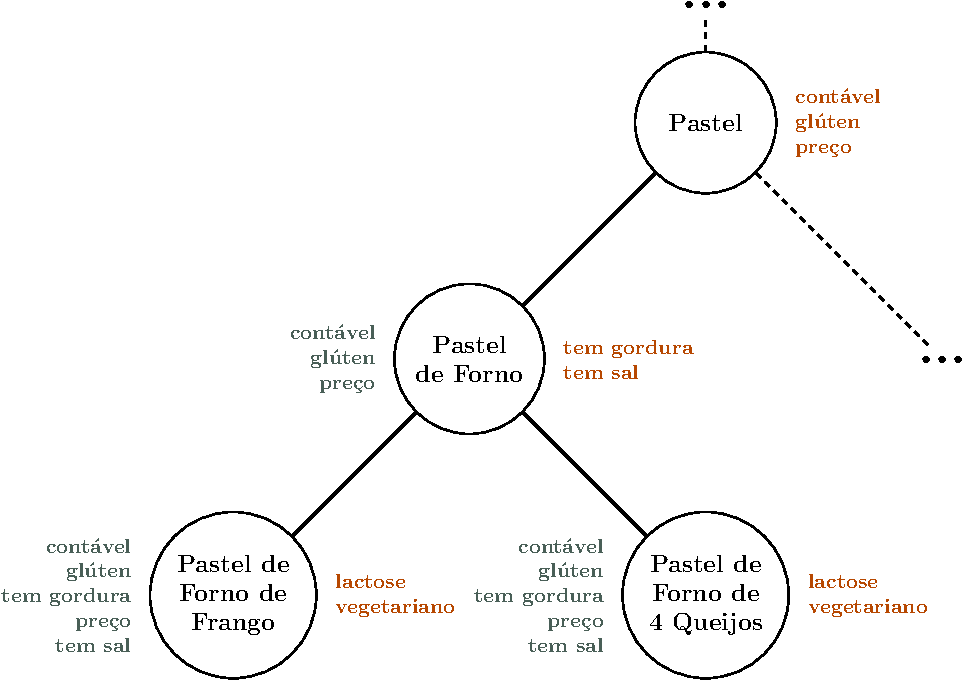
\includegraphics[width=0.6\linewidth]{./pdf/tikz/toptop-1.pdf}
\end{figure}

O processo de aquisição de todas as propriedades de um produto começou com o caminhamento do nodo raiz até os nodos folhas da árvore da ontologia. Observando a Figura \ref{fig:integracao-2}, é possível notar que algumas propriedades devem ser passadas para os nodos filhos durante o percorrimento de cima pra baixo:

\begin{figure}[H]
	\centering
	\caption[Integração da Ontologia -- Passos 1--4]{Passos 1--4 -- Os atributos das classes superiores são passados para suas filhas. Os textos em tom acinzentado representam os atributos herdados de forma anônima e os textos em laranja representam os atributos das classes}
	\label{fig:integracao-2}
	\subfigure[c][Passo 1 -- A classe \emph{Pastel de Forno} recebe os atributos da classe \emph{Pastel}]
	{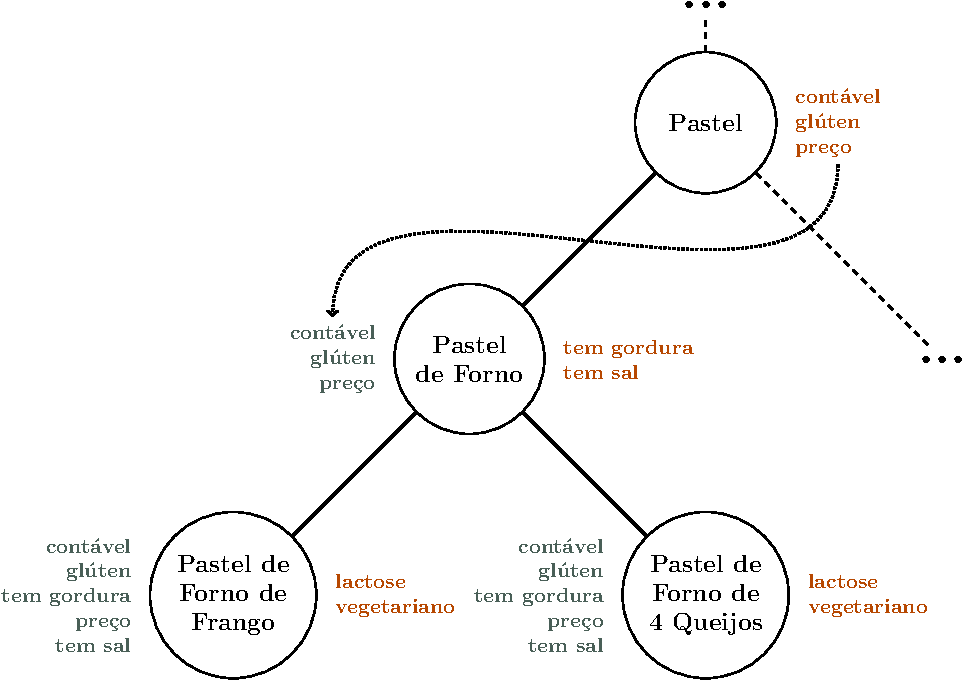
\includegraphics[width=0.45\textwidth]{./pdf/tikz/topdown-1.pdf}}
	\qquad
	\subfigure[c][Passo 2 -- Os atributos recebidos são armazenados em sua própria lista de atributos]
	{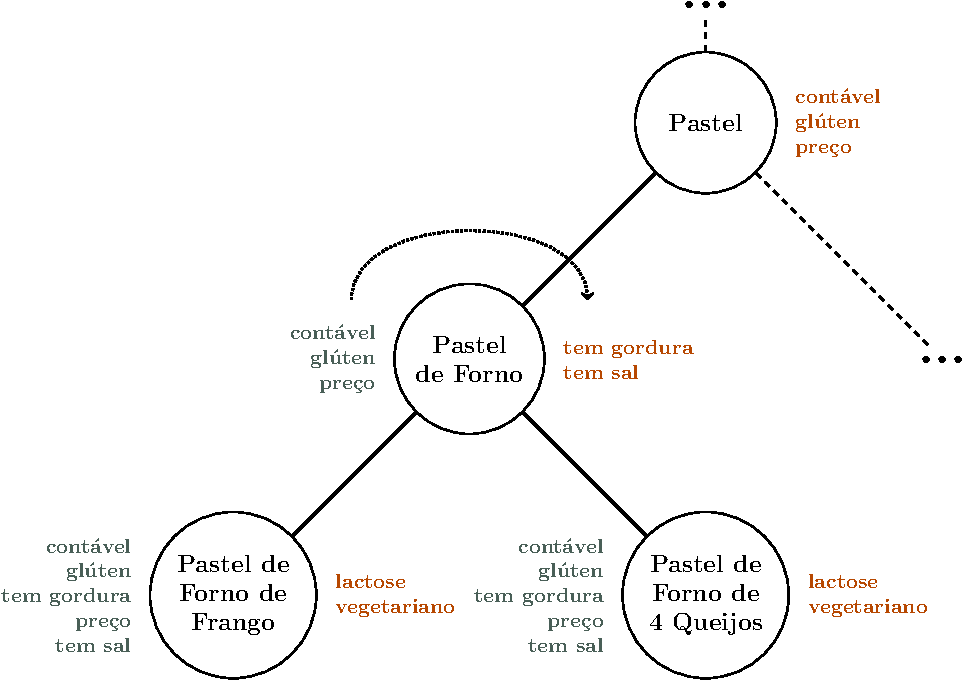
\includegraphics[width=0.45\textwidth]{./pdf/tikz/topdown-2.pdf}}
	\qquad
	\subfigure[c][Passo 3 -- O mesmo processo se repete, agora com a classe \emph{Pastel de Forno}]
	{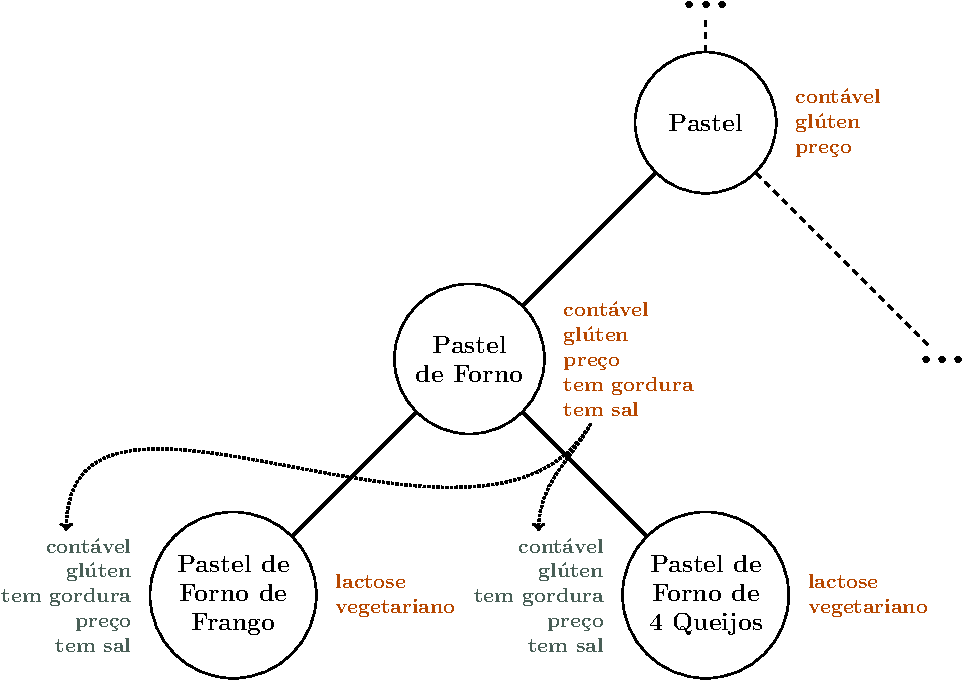
\includegraphics[width=0.45\textwidth]{./pdf/tikz/topdown-3.pdf}}
	\qquad
	\subfigure[c][Passo 4 -- Os atributos recebidos são armazenados em sua própria lista de atributos]
	{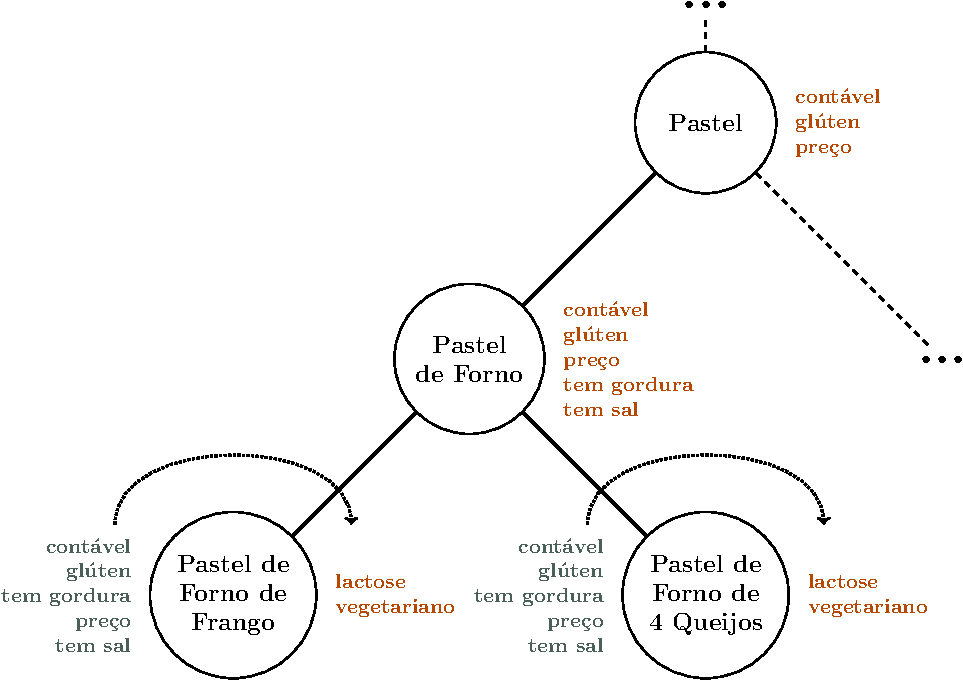
\includegraphics[width=0.45\textwidth]{./pdf/tikz/topdown-4.pdf}}
\end{figure}

Esse processo de repercussão de características é feito com o uso de uma estrutura de dados HashMap, a qual armazena as propriedades do nodo atual e seus valores (verdadeiro ou falso) e propaga estes dados para seus nodos filhos. Desta forma, ao chegar em um nodo folha, seu mapa de propriedades deve estar totalmente preenchido, como mostrado na Figura \ref{fig:integracao-3}:

\begin{figure}[H]
	\centering
	\caption[Integração da Ontologia -- Passo 5]{Passo 5 -- Todos os atributos foram transferidos às classes sucessoras. Os textos em tom acinzentado representam os atributos herdados de forma anônima e os textos em laranja representam os atributos das classes}
	\label{fig:integracao-3}
	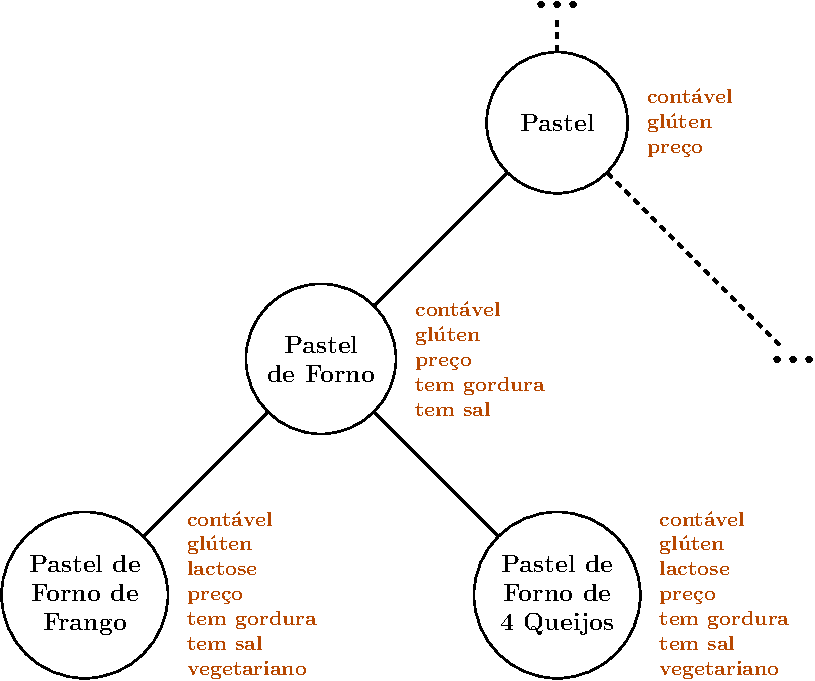
\includegraphics[width=0.55\linewidth]{./pdf/tikz/topdown-5.pdf}
\end{figure}

Nota-se que, apesar dos nodos folhas possuírem todos os valores de suas propriedades, o mesmo não ocorre com as classes mais gerais. Sendo assim, torna-se necessário um novo caminhamento, desta vez do nodo folha ao nodo raiz, buscando atribuir aos primeiros nodos as características que estão presentes em seus filhos. Para isso, foi desenvolvido um critério de atribuição de valores, buscando armazenar apenas os valores que seriam relevantes à aplicação. Este processo é demonstrado na Figura \ref{fig:integracao-4}. 

\begin{figure}[H]
	\centering
	\caption[Integração da Ontologia -- Passos 6--10]{Passos 6--10 -- Os atributos são repassados das folhas à raiz}
	\label{fig:integracao-4}
	\subfigure[c][Passo 6 -- União entre os atributos das classes folhas e os de sua classe mãe]
	{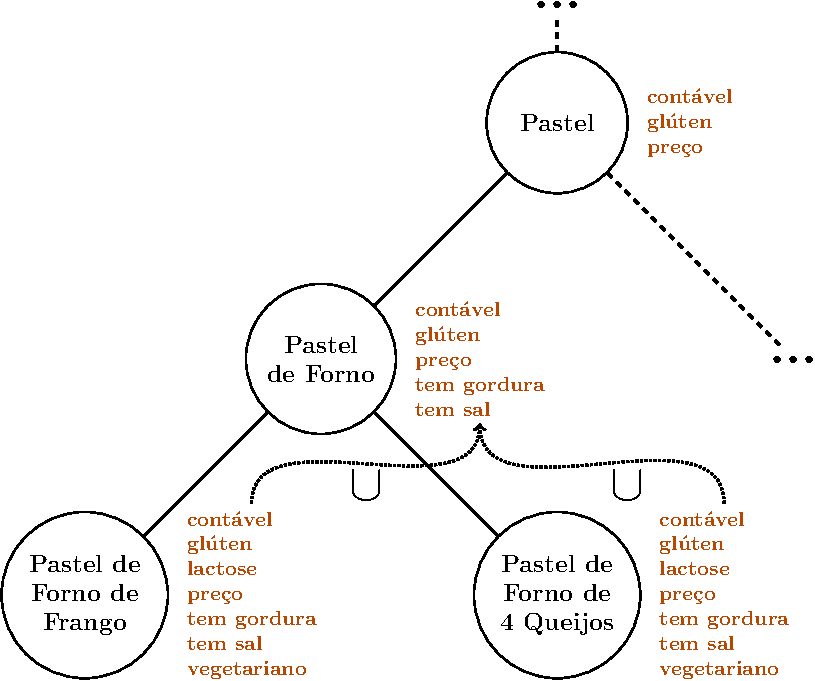
\includegraphics[width=0.45\textwidth]{./pdf/tikz/bottomup-1.pdf}}
	\qquad
	\subfigure[c][Passo 7 -- Classe \emph{Pastel de Forno} agora possui os atributos de suas filhas]
	{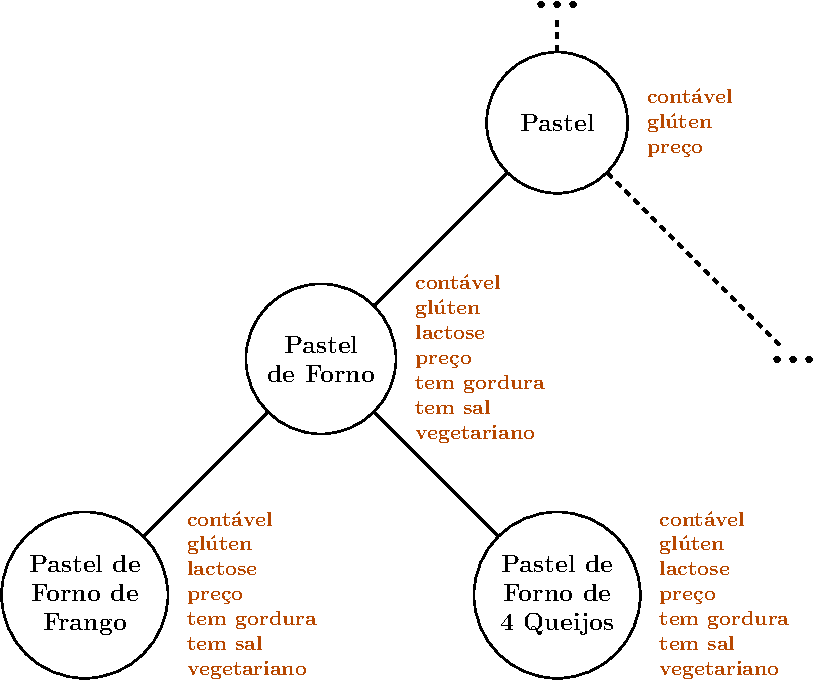
\includegraphics[width=0.45\textwidth]{./pdf/tikz/bottomup-2.pdf}}
	\qquad
	\subfigure[c][Passo 8 -- Classe \emph{Pastel de Forno} propaga estas informações a sua classe mãe]
	{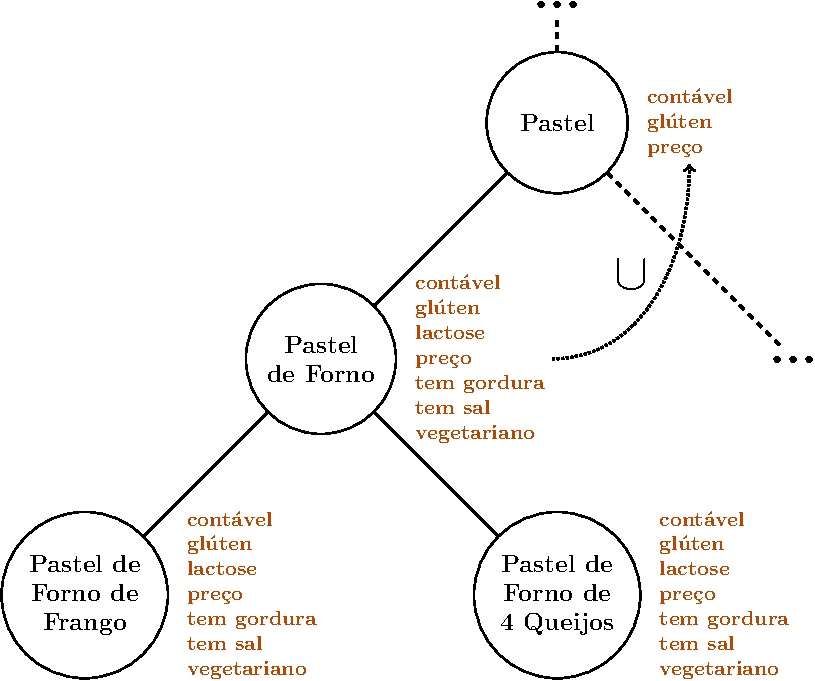
\includegraphics[width=0.45\textwidth]{./pdf/tikz/bottomup-3.pdf}}
	\qquad
	\subfigure[c][Passo 9 -- Classe \emph{Pastel} agora possui os atributos de suas filhas]
	{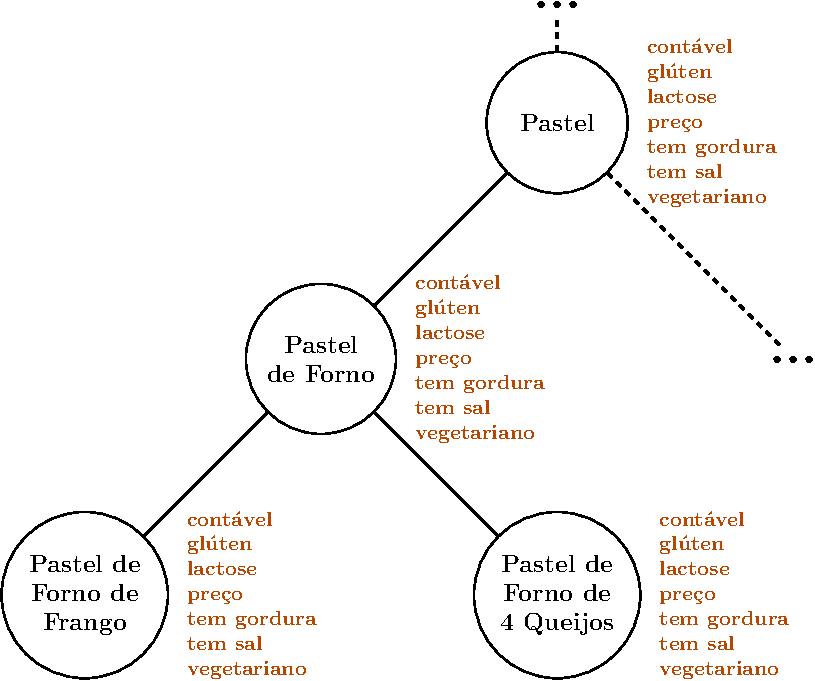
\includegraphics[width=0.45\textwidth]{./pdf/tikz/bottomup-4.pdf}}
	\qquad
	\subfigure[c][Passo 10 -- Classe \emph{Pastel} propaga estas informações para suas classes antecessoras]
	{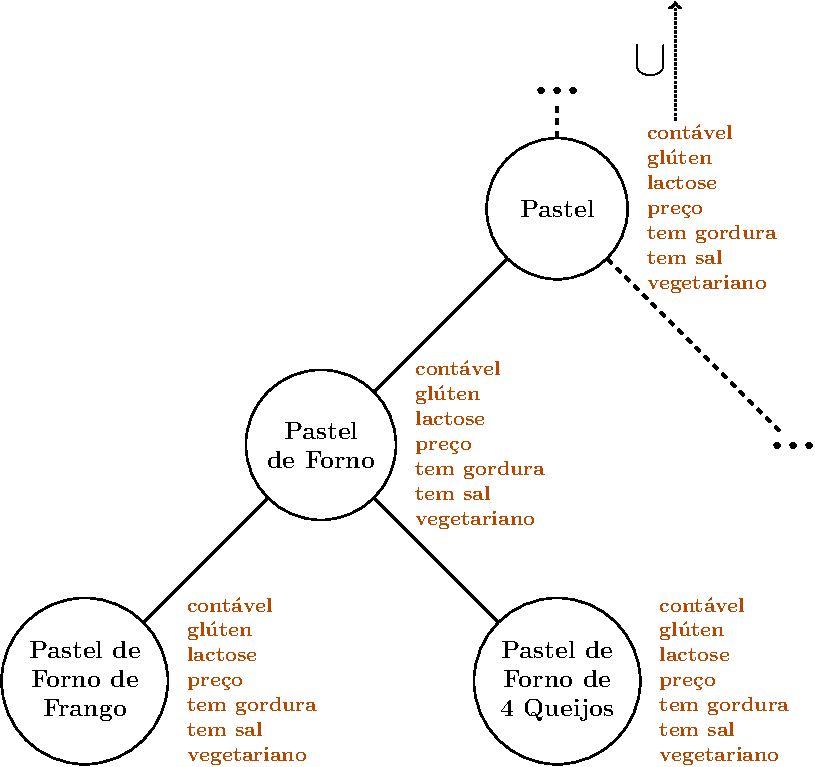
\includegraphics[width=0.45\textwidth]{./pdf/tikz/bottomup-5.pdf}}
\end{figure}

\section{Aplicação}

Sendo possível o acesso à ontologia através da aplicação, bastou-se incorporar os demais elementos. Primeiramente, a aplicação apresenta uma tela inicial (Figura \ref{fig:cardapio-virtual-1}(a)), com a listagem dos todos os restaurantes armazenados no sistema e dos restaurantes favoritos do usuário, uma barra de busca e um botão para a tela de ajuda. Ao clicar no botão de busca, a barra se expande, exibindo o campo de busca com suas opções de pesquisa, as quais vão sendo alteradas à medida que o usuário insere caracteres neste campo. Além de busca por digitação, existe, também, a opção de procurar um restaurante através do modo de busca por voz (Figura \ref{fig:cardapio-virtual-1}(b)).

\begin{figure}[H]
	\centering
	\caption[Telas da Aplicação 1--3]{Tela inicial da aplicação e seu sistema de buscas}
	\label{fig:cardapio-virtual-1}
	\subfigure[c][Tela inicial da aplicação]
	{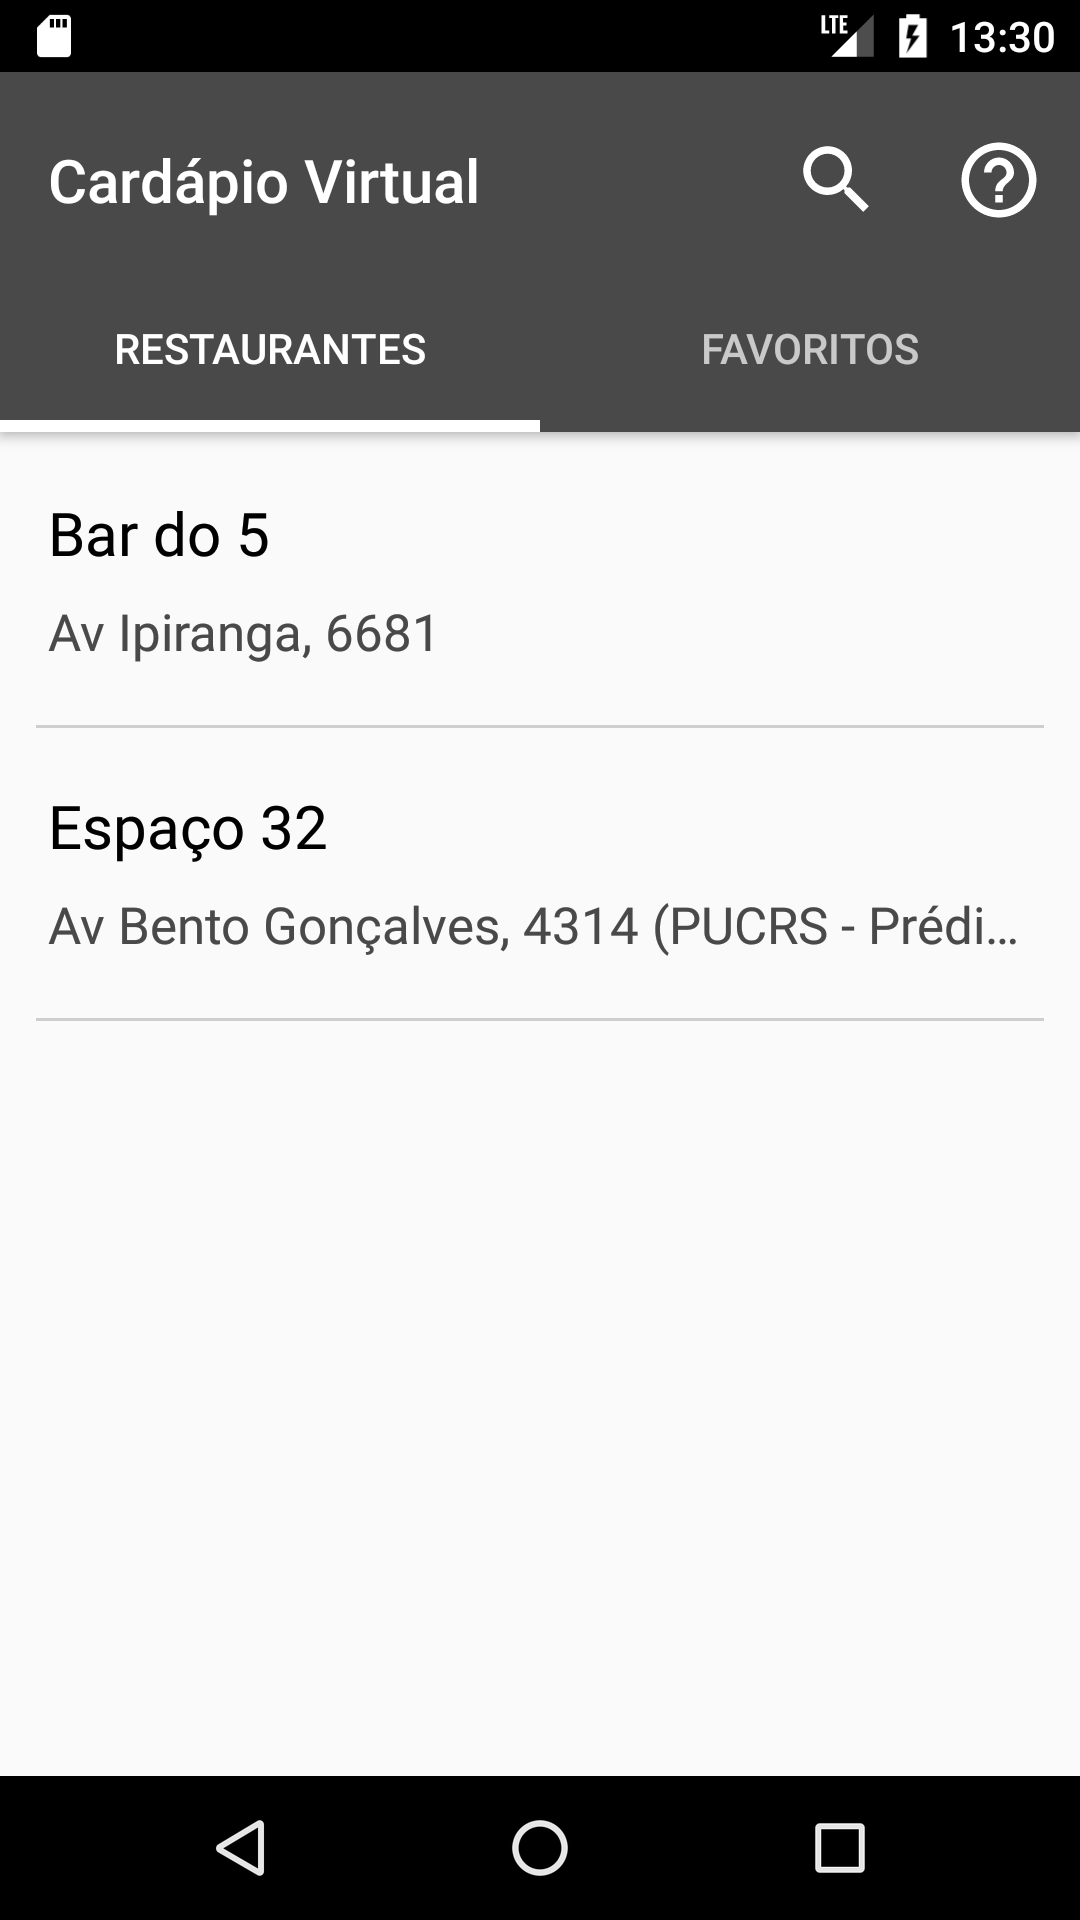
\includegraphics[width=0.29\textwidth]{./fig/cardapio-virtual/tela-inicial-1.png}}
	\qquad
	\subfigure[c][Barra de buscas de restaurantes]
	{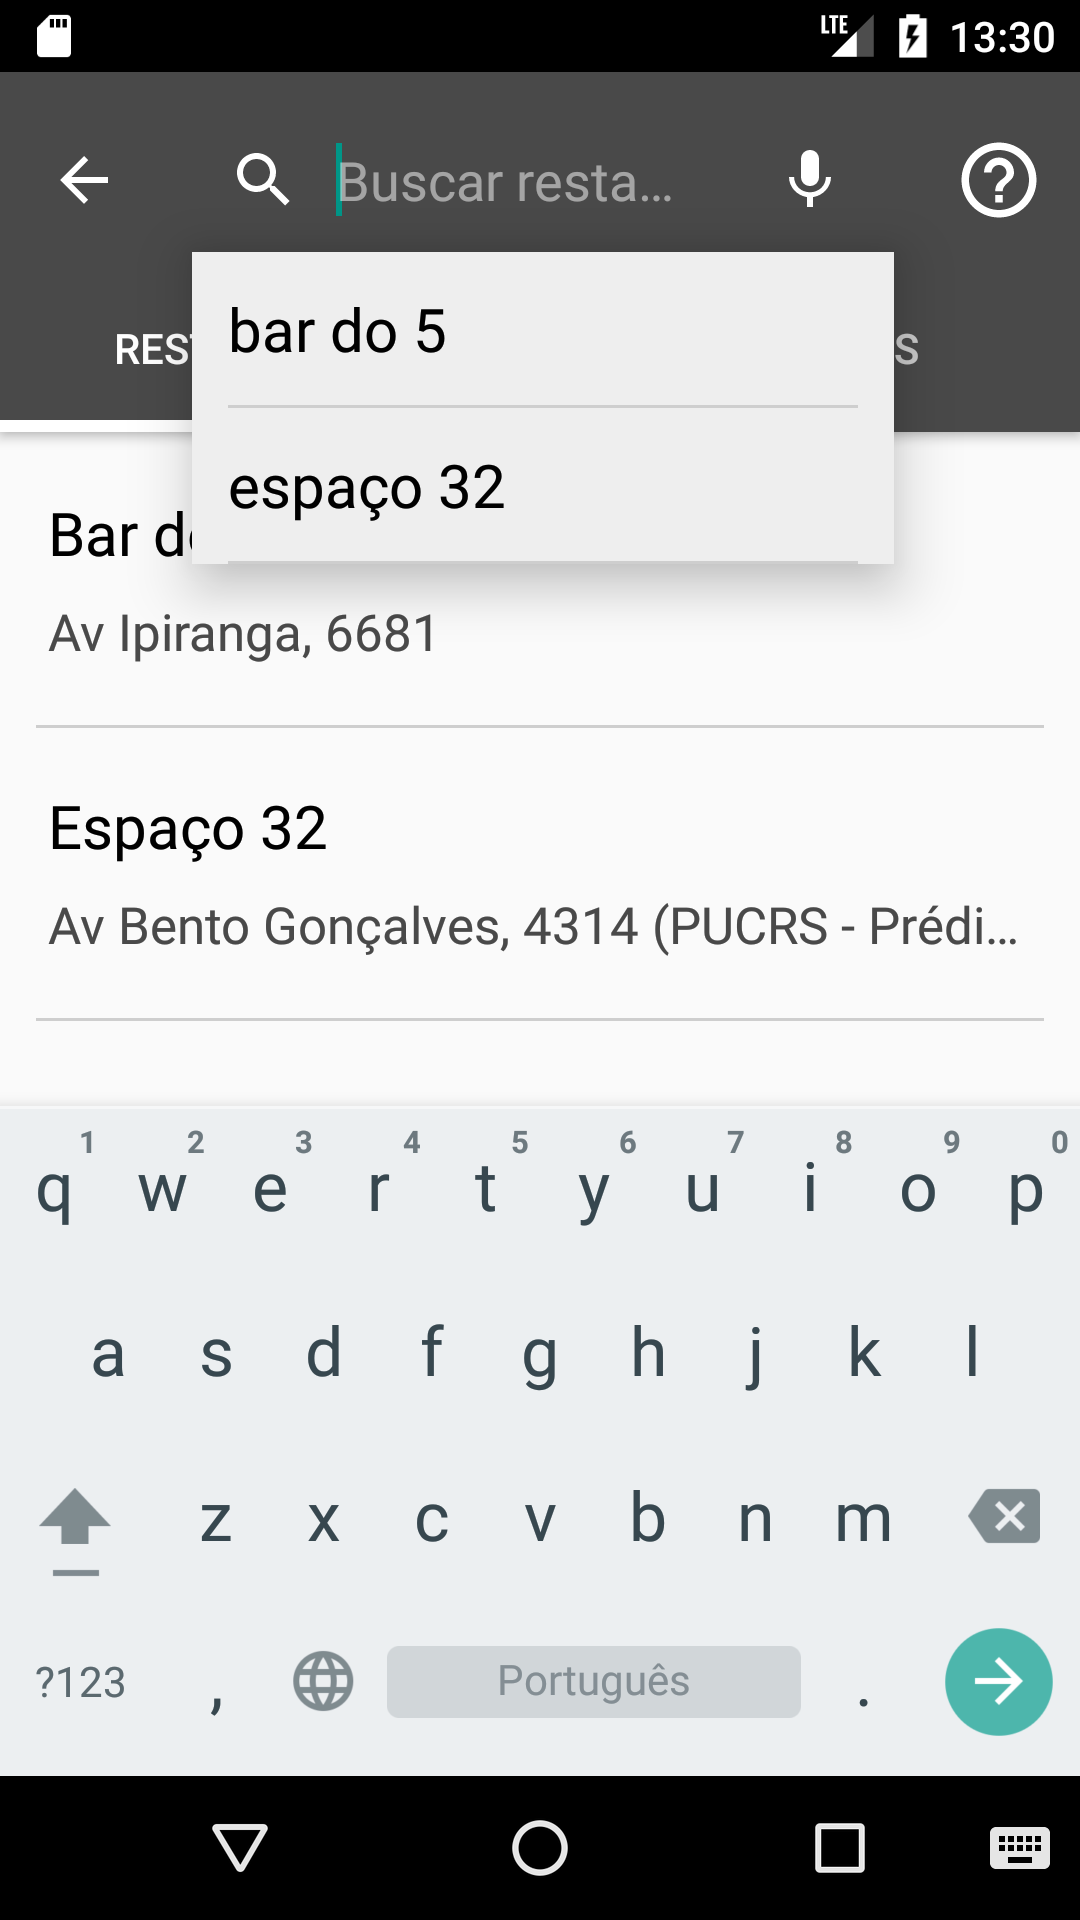
\includegraphics[width=0.29\textwidth]{./fig/cardapio-virtual/tela-inicial-2-busca.png}}
	\qquad
	\subfigure[c][Resultado da busca por "es"\ no sistema]
	{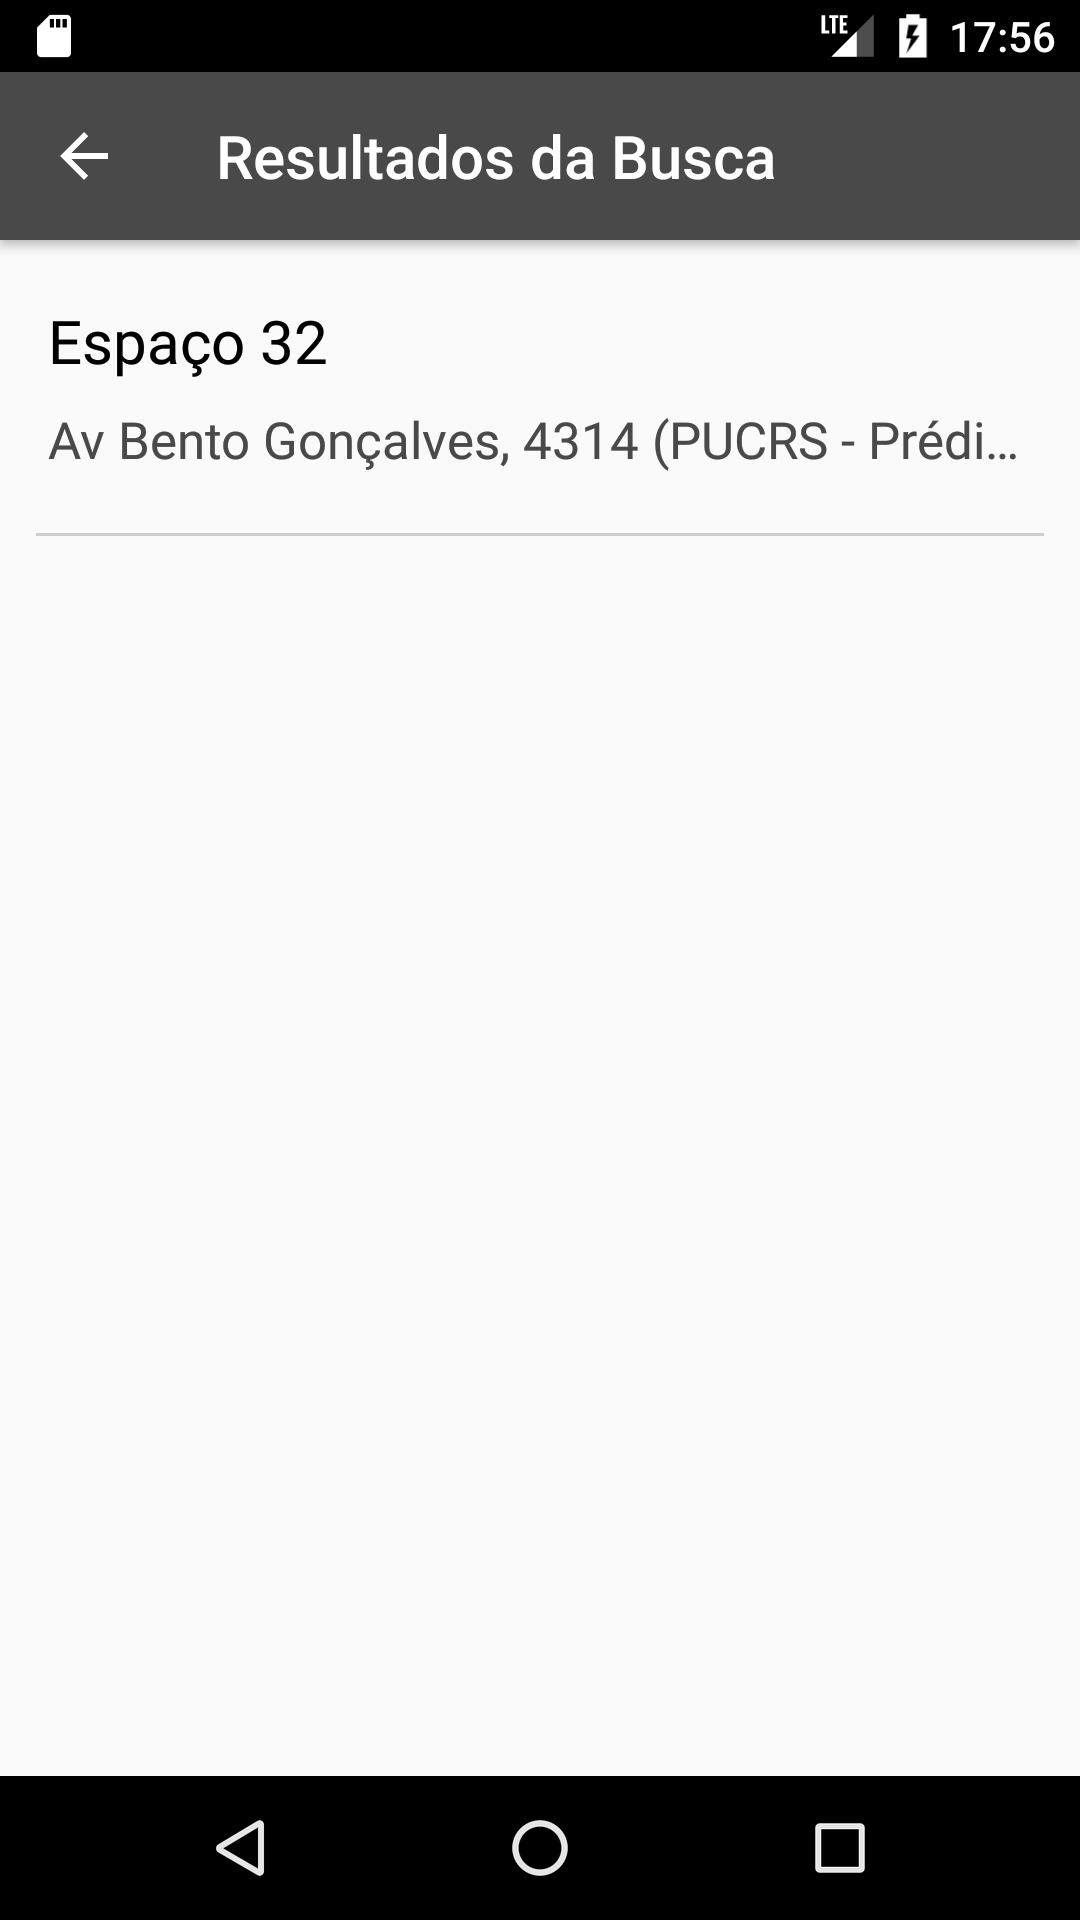
\includegraphics[width=0.29\textwidth]{./fig/cardapio-virtual/tela-busca.png}}
\end{figure}

A partir da tela principal (Figura \ref{fig:cardapio-virtual-1}(a)), o usuário é capaz de:
\begin{itemize}
	\item Selecionar um restaurante e acessar suas informações adicionais;
	\item Fazer uma busca e selecionar um dos restaurantes sugeridos pela barra de pesquisa, sendo levado para a tela de informações adicionais do local;
	\item Fazer uma busca e ir para a tela de resultado de buscas; e
	\item Acessar a tela de ajuda.
\end{itemize}
A tela de resultado da busca (figura \ref{fig:cardapio-virtual-1}(c)) apenas lista os resultados que se encaixam com a pesquisa, possibilitando que o usuário selecione um dos locais ou volte para a tela inicial. A tela de informações adicionais de um restaurante, mostrada na Figura \ref{fig:cardapio-virtual-2}(a), apresenta uma breve descrição do local; suas informações básicas, como telefone e e-mail; acesso ao seu cardápio e um botão que possibilita ao usuário favoritar ou desfavoritar o local. Por fim, a tela de ajuda, apresentada na Figura \ref{fig:cardapio-virtual-2}(b)), exibe algumas perguntas e respostas que visam auxiliar o usuário durante sua experiência com a aplicação.

\begin{figure}[H]
	\centering
	\caption[Telas da Aplicação 4--5]{Telas de informações adicionais dos restaurantes e sistema de ajuda}
	\label{fig:cardapio-virtual-2}
	\subfigure[c][Tela de informações adicionais do restaurante Espaço 32]
	{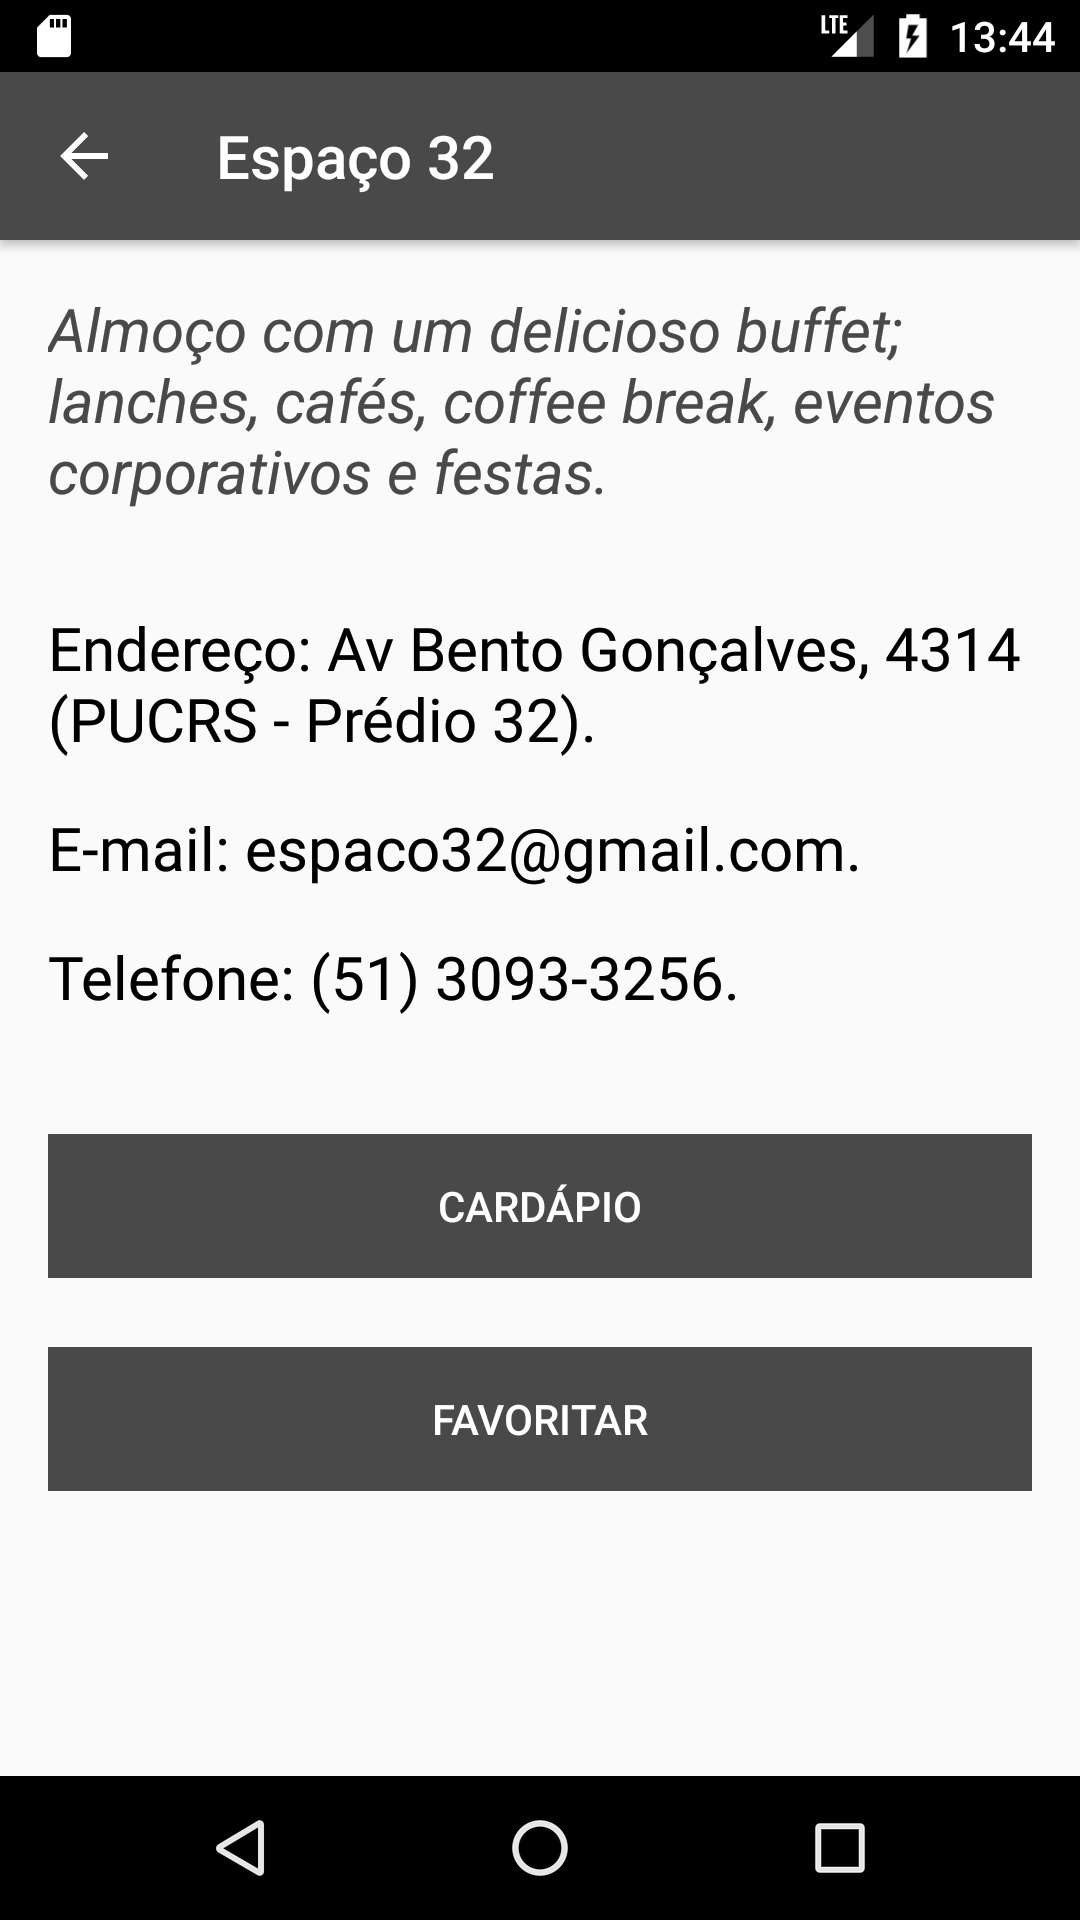
\includegraphics[width=0.3\textwidth]{./fig/cardapio-virtual/info-restaurante-1.png}}
	\qquad
	\subfigure[c][Tela de ajuda]
	{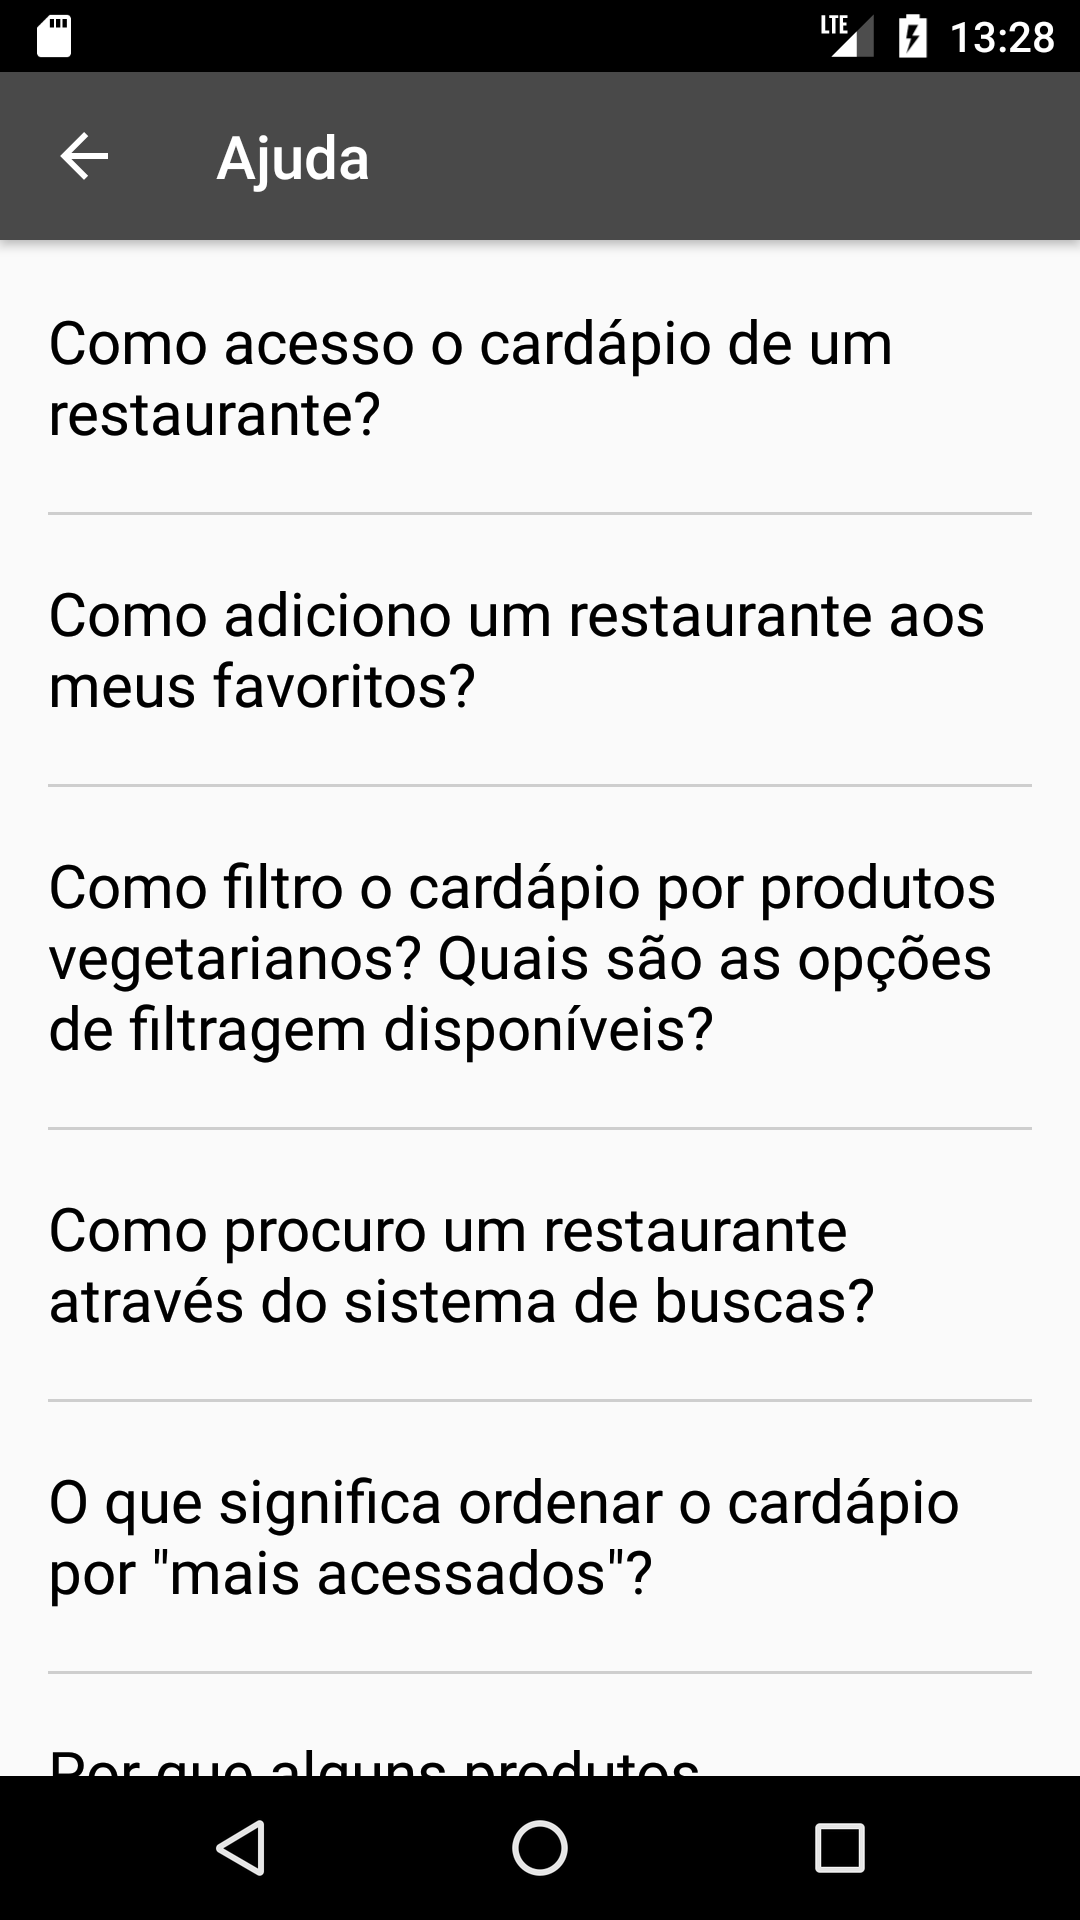
\includegraphics[width=0.3\textwidth]{./fig/cardapio-virtual/ajuda-1.png}}
\end{figure}

Seguindo o fluxo da aplicação, a próxima tela a ser exibida é a tela do menu (figura \ref{fig:cardapio-virtual-3}(c)), a qual é acionada quando o usuário seleciona o cardápio de um restaurante. Esta tela apresenta os produtos disponíveis no local agrupados por categorias. Há também dois métodos de disposição dos itens do cardápio: o método de filtragem e o de ordenação. O primeiro permite que o usuário filtre os produtos do cardápio a partir de um ou mais dos seguintes critérios: sem glúten, sem lactose, vegetarianos, com pouca gordura e com pouco sal. Já o segundo permite ao usuário que os produtos sejam dispostos em ordem alfabética ou em ordem de acesso -- permitindo, assim, que os produtos mais acessados sejam facilmente encontrados nas próximas consultas. Estes métodos são apresentados nas Figuras \ref{fig:cardapio-virtual-3}(e) e \ref{fig:cardapio-virtual-3}(f). Por fim, ao selecionar um produto da lista, suas informações adicionais, ou seja, seus ingredientes, seu preço e sua quantidade disponível no local, são exibidas na tela, como demonstrado na Figura \ref{fig:cardapio-virtual-4}(g). Sendo assim, o usuário tem acesso aos produtos dos restaurantes, bem como as informações básicas que necessita para escolher qual produto mais lhe agrada.

\begin{figure}[H]
	\centering
	\caption[Telas da Aplicação 6--10]{Demais telas da aplicação}
	\label{fig:cardapio-virtual-3}
	\subfigure[c][Tela inicial do cardápio]
	{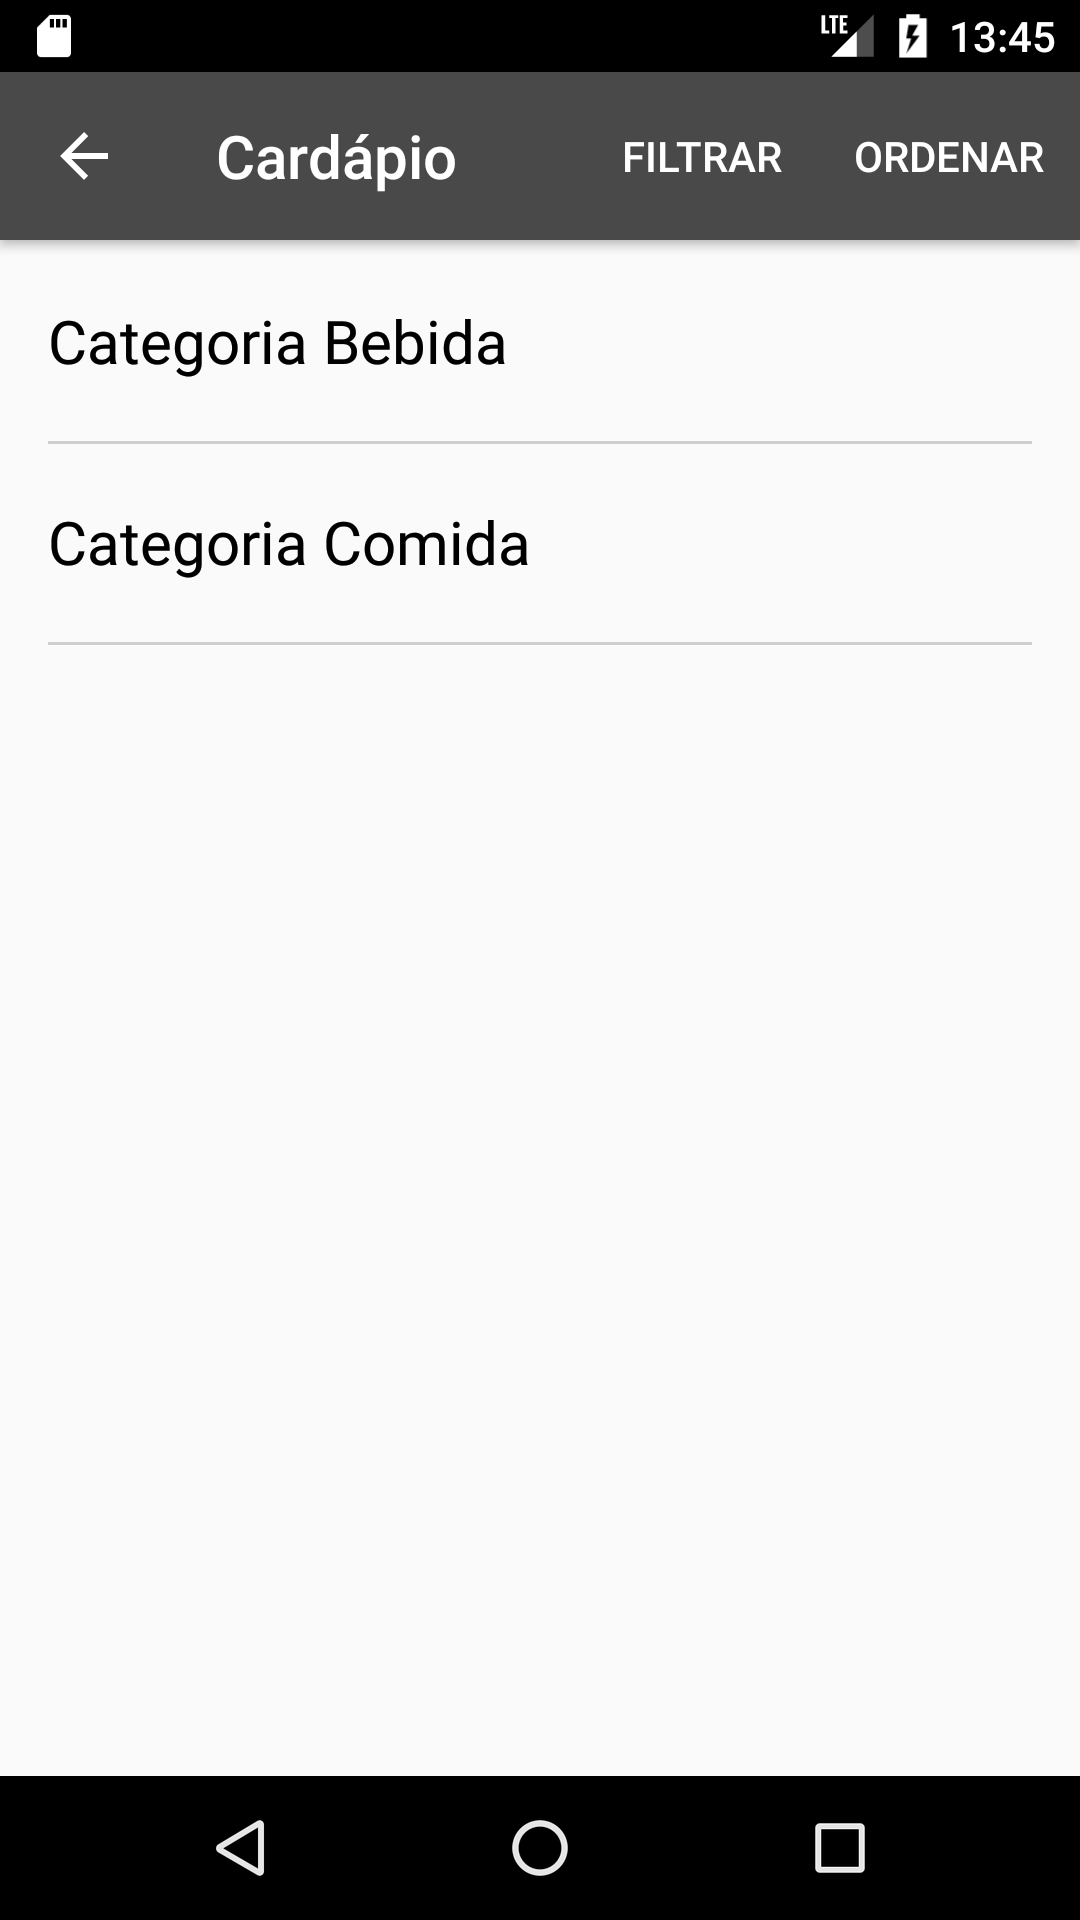
\includegraphics[width=0.3\textwidth]{./fig/cardapio-virtual/cardapio-1.png}}
	\qquad
	\subfigure[c][Tela de lanches do cardápio]
	{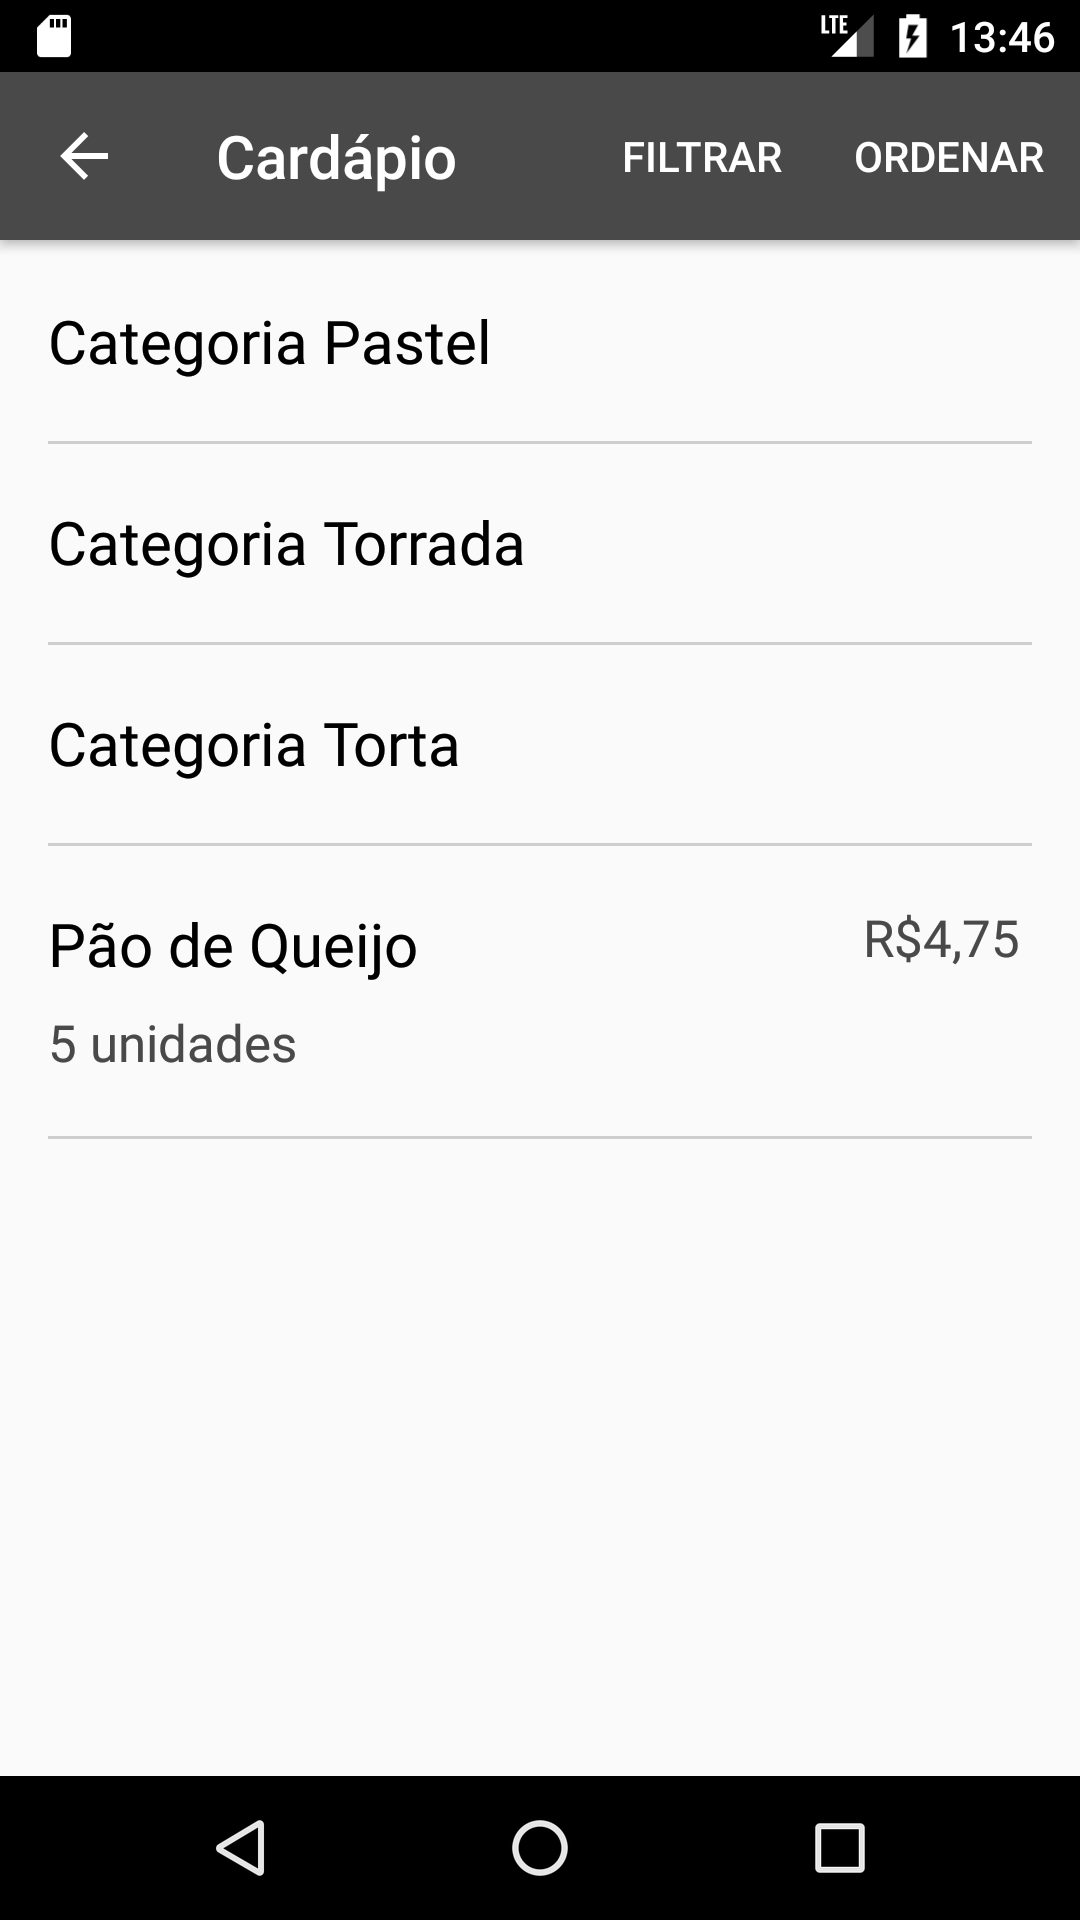
\includegraphics[width=0.3\textwidth]{./fig/cardapio-virtual/cardapio-2.png}}
	\qquad
	\subfigure[c][Filtros do cardápio]
	{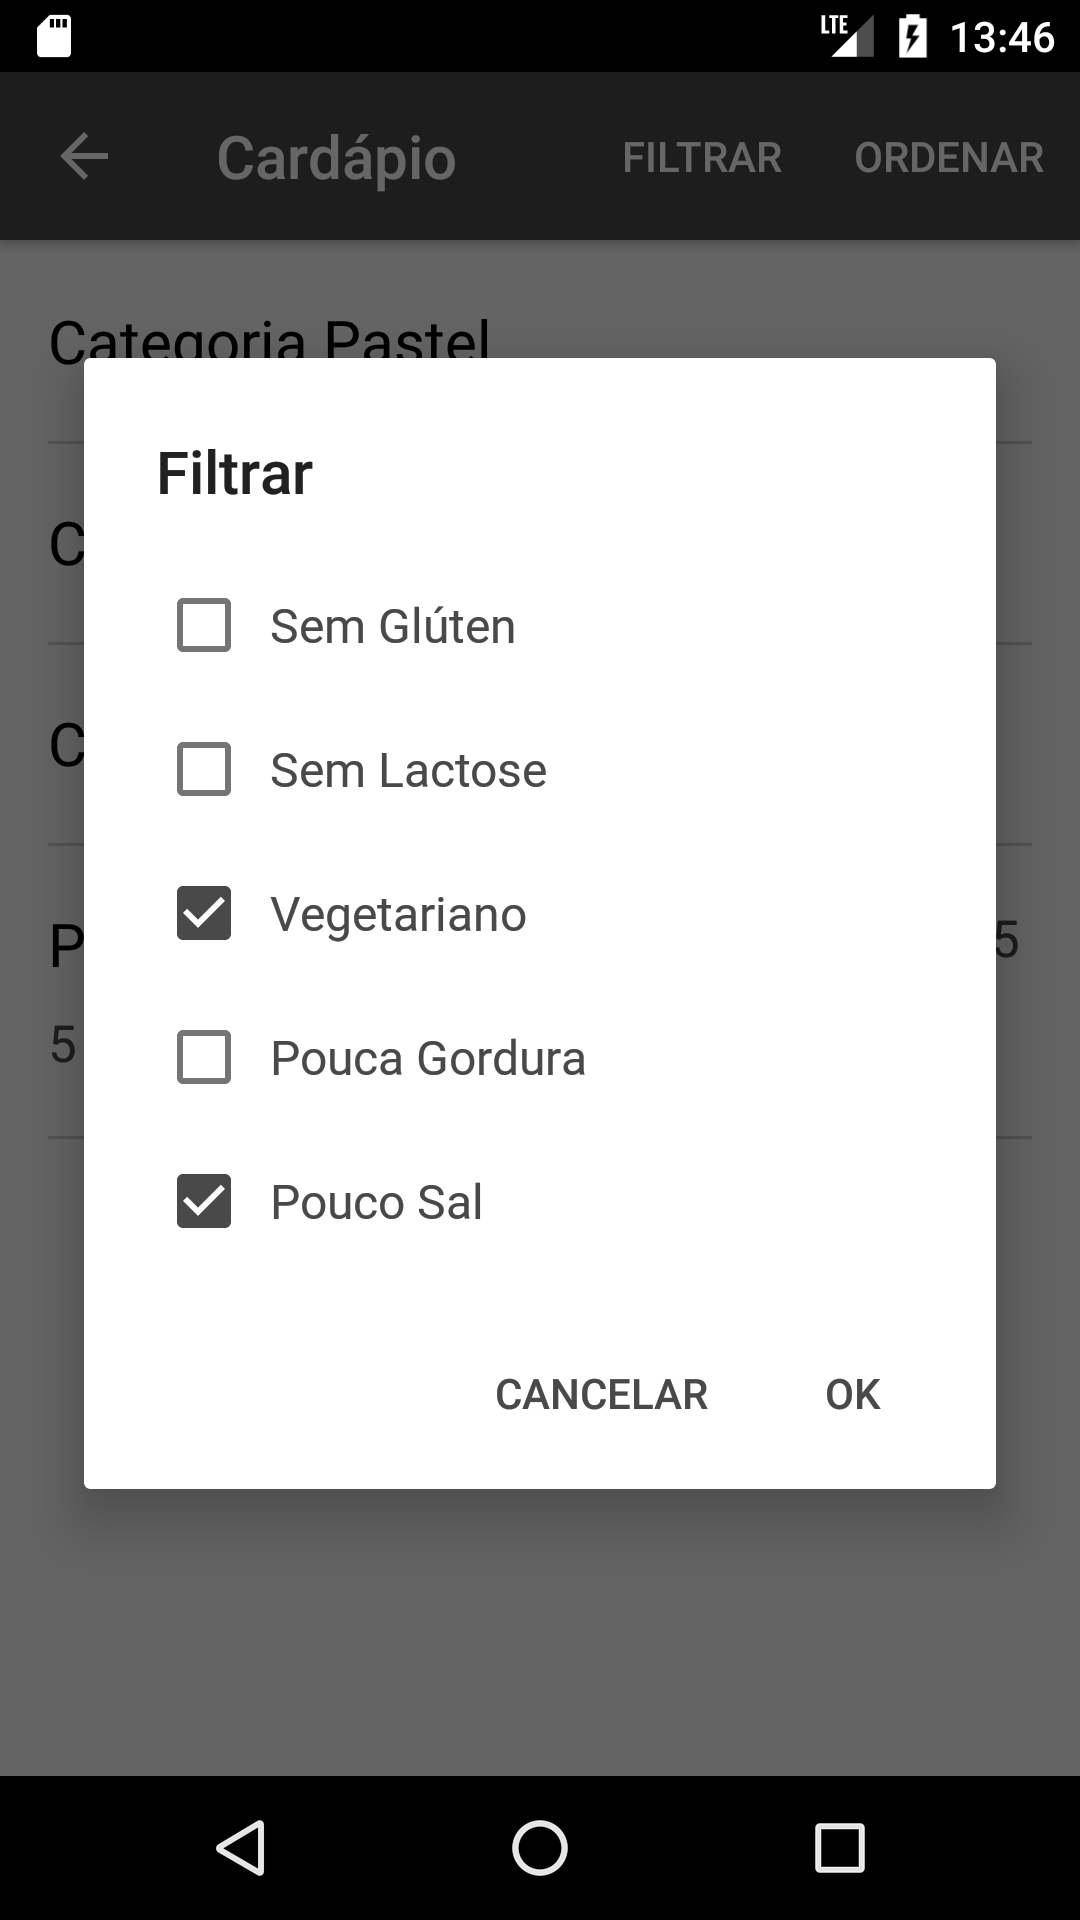
\includegraphics[width=0.3\textwidth]{./fig/cardapio-virtual/filtrar-1.png}}
	\qquad
	\subfigure[c][Ordenação do cardápio]
	{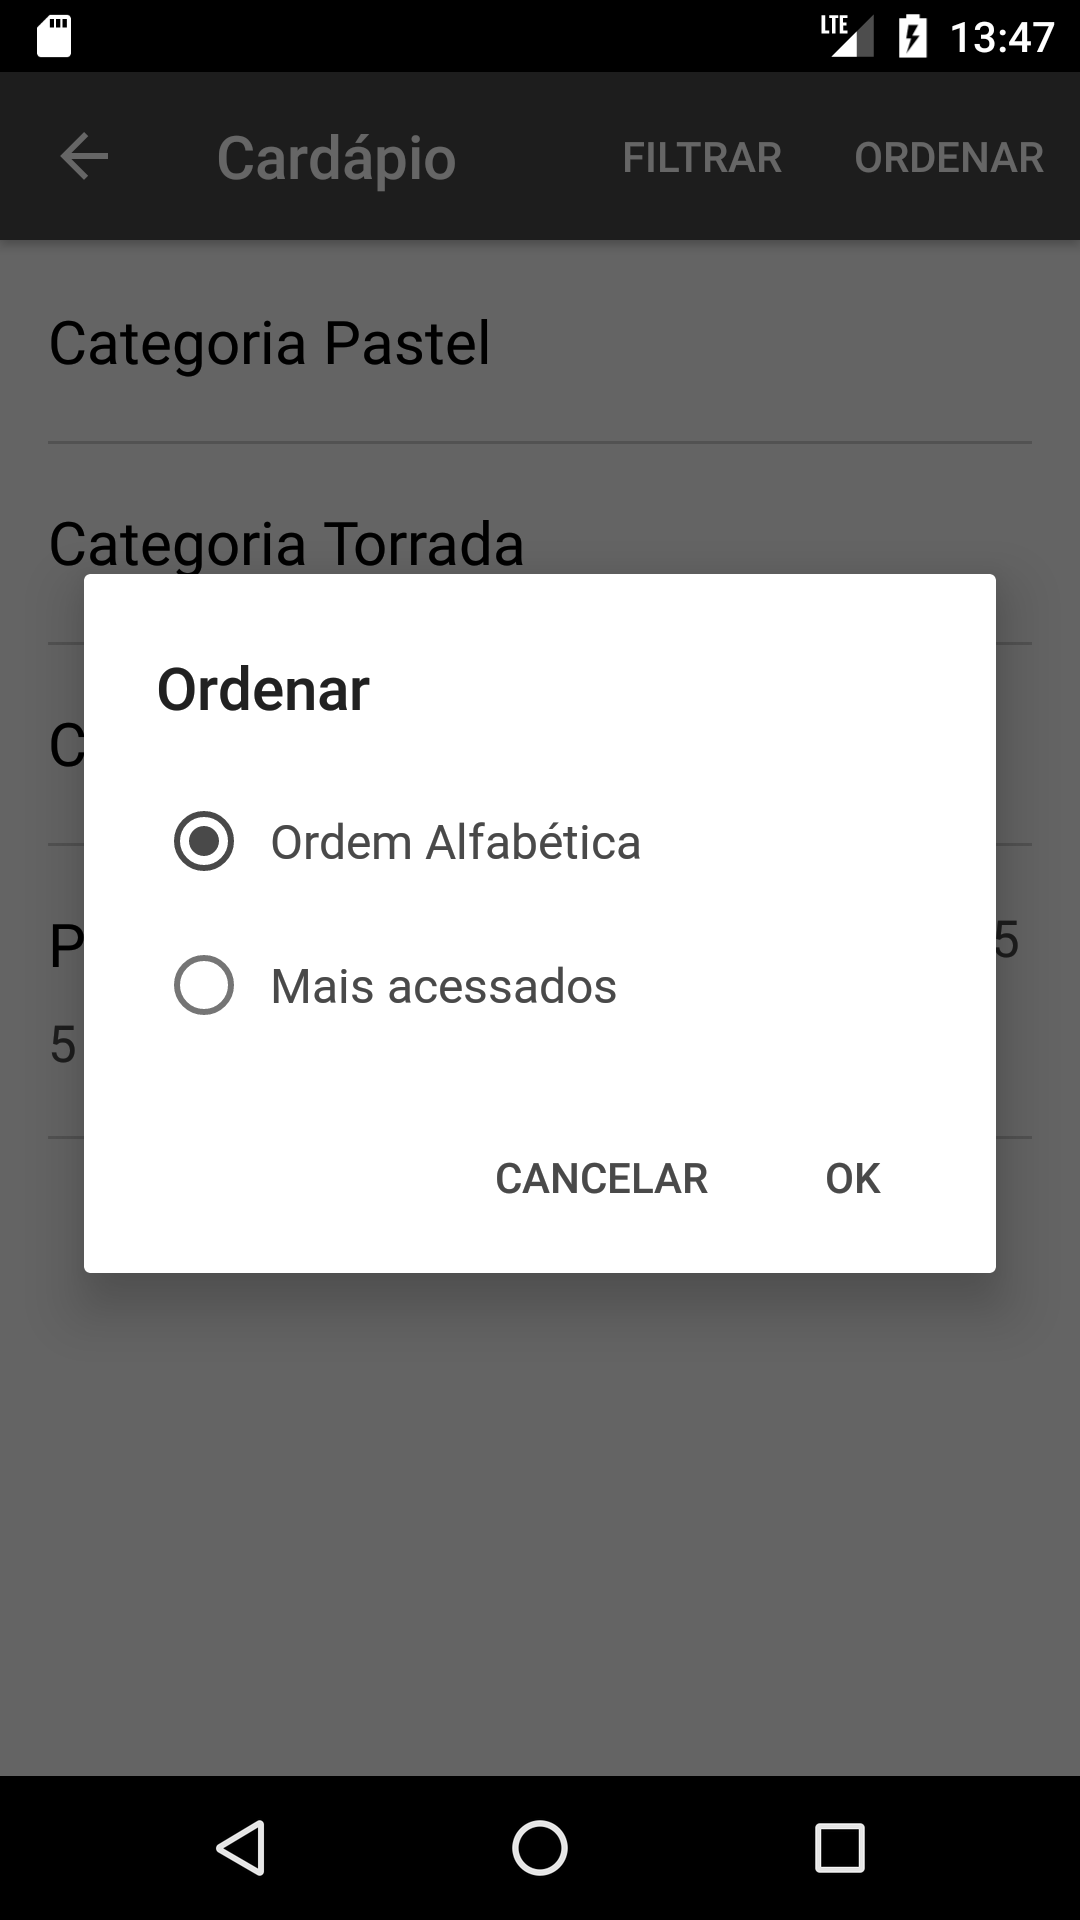
\includegraphics[width=0.3\textwidth]{./fig/cardapio-virtual/ordenar-1.png}}
\end{figure}

\begin{figure}[H] \ContinuedFloat
	\centering
	\caption[]{Continuação da página anterior}
	\label{fig:cardapio-virtual-4}
	\subfigure[c][Informações adicionais do produto]
	{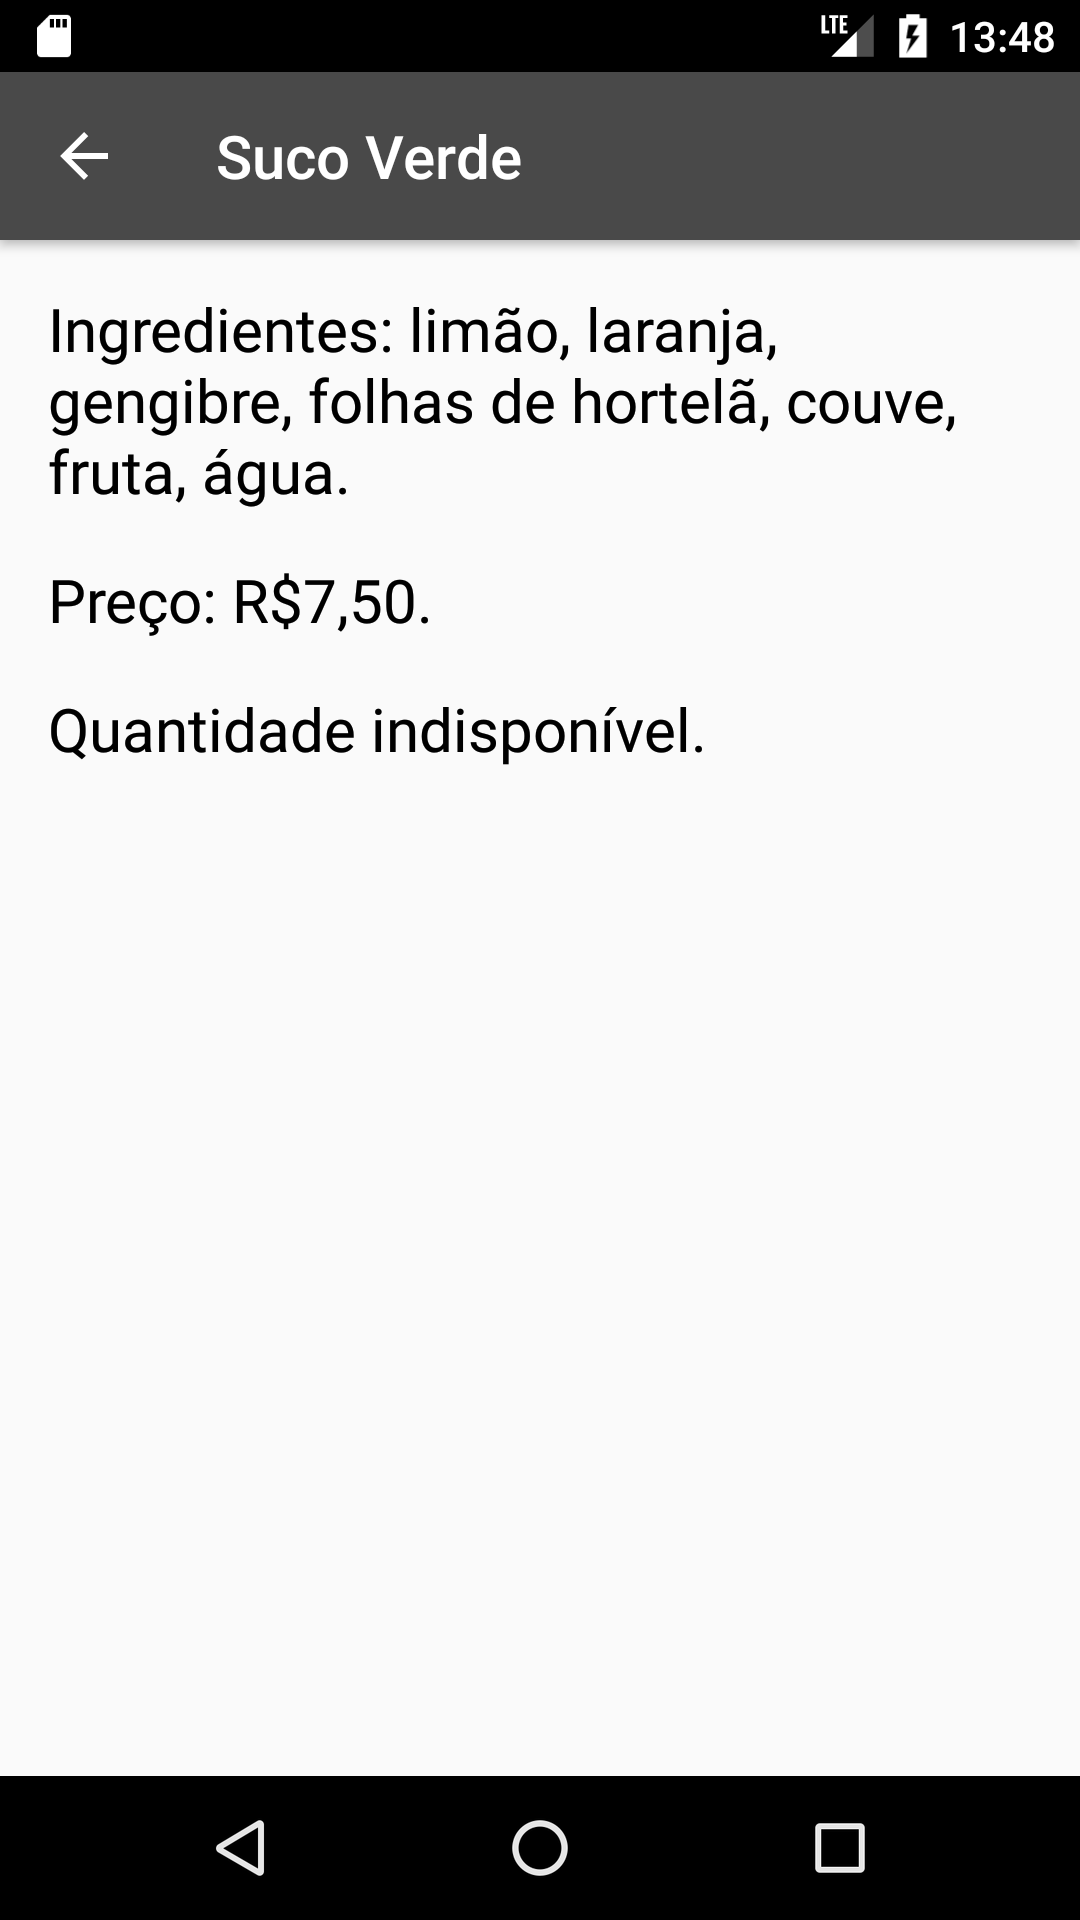
\includegraphics[width=0.3\textwidth]{./fig/cardapio-virtual/produto-1.png}}
\end{figure}

		\chapter{\label{chap:avaliacao}Avaliação}

O término do desenvolvimento de uma aplicação não inflige na sua utilização imediata pelo o usuário. Antes de lançá-la para o mercado ou para o ambiente onde será aplicada, é de extrema importância que se testem fatores relacionados à interação entre a aplicação e o usuário (Prates e Barbosa, 2003). Uma vez que avaliação da interface transparece aspectos da usabilidade do sistema, seus resultados contribuem para a diminuição do número de erros e aumento da produtividade e da satisfação do usuário (Winckler e Pimenta, 2002)\nocite{WINCKLER2002}. Além disso, Prates e Barbosa (2003) ressaltam que estas avaliações têm por objetivo identificar as necessidades do usuário, entender como a interface o afeta, quantificar aspectos de usabilidade e conformidade com padrões ou conjuntos de heurísticas, entre outros.

Para a aplicação destas avaliações, busca-se usuários que não tenham interação prévia com a aplicação. Desenvolvedores e outros membros da equipe de desenvolvimento de um projeto devem ter em mente que os usuários reais de suas aplicações, muitas vezes, possuem uma visão diferente e podem salientar pontos que não foram percebidos pela equipe (Prates e Barbosa, 2003). Através do teste com uma pessoa que se encaixa neste perfil, torna-se viável a análise qualitativa do produto criado.

Há diversas formas e práticas para se avaliar a interface de um sistema. De acordo com Maguire\footnote{Maguire, M., 2001, Methods to support human-centered design. Em \emph{International Journal of Human-Computer Studies}, vol. 55, no. 4, pp. 587-634. Academic Press, Inc., Duluth, MN, EUA.} (2001, citado por Wich e Kramer, 2015\nocite{WICH2015}), não há necessidade de aplicar todas os métodos disponíveis, mas sim aqueles que melhor convêm com os objetivos do projeto. Sendo assim, neste trabalho, serão aplicados uma avaliação heurística, uma lista de medidas a serem avaliadas (\emph{checklist}) e um questionário.

\section{Avaliação Heurística}

Seguindo as heurísticas de Nielsen (1995)\nocite{NIELSEN1995}, este método permite que o usuário encontre problemas relacionados à usabilidade do sistema avaliado (Prates e Barbosa, 2003). Nessa etapa, o próprio desenvolvedor pode exercer o papel de avaliador e usuários reais da aplicação não estão envolvidos. Winckler e Pimenta (2002) recomendam que 3 a 5 avaliadores analisem, de forma individual, a interface apresentada, para que os dados sejam mais consistentes.

Os dez “princípios gerais para design de interação” (Nielsen, 1995) são:
\begin{description}
	\item [Visibilidade do estado do sistema] o sistema deve manter o usuário informado sobre o quê está acontecendo através de retornos em tempo adequado.
	\item [Nivelamento entre o sistema e o mundo real] o sistema deve falar a língua do usuário, com palavras, frases e conceitos que sejam familiares, em vez de usar termos técnicos. A informação deve ser apresentada de forma natural e lógica.
	\item [Controle e liberdade] frequentemente, usuários escolhem alguma opção por engano. Dê suporte para ações de \emph{desfazer} e \emph{refazer}.
	\item [Consistência e padrões] seja consistente e siga um padrão. Usuários não devem ter que adivinhar se diferentes palavras, situações ou ações executam a mesma função.
	\item [Prevenção de erro] previna que erros aconteçam. Elimine condições propensas a falhas e apresente uma opção de confirmação ao usuário antes que ele execute ações de risco.
	\item [Reconhecimento, não relembrança] o usuário não deveria ter que recordar informações de telas anteriores. Instruções e opções devem estar visíveis ou serem facilmente acessadas.
	\item [Flexibilidade e eficiência de uso] usuários com experiência possuem um ritmo diferente dos principiantes. Permita que o sistema ofereça caminhos alternativos para ambos os tipos de usuários.
	\item [Estética e design minimalista] diálogos não devem conter informações irrelevantes. Informações desnecessárias competem com as informações úteis e as tornam menos visíveis.
	\item [Ajude o usuário a reconhecer, diagnosticar e recuperar-se de erros] mensagens de erro devem ser apresentadas em uma linguagem acessível -- sem códigos --, indicando o problema e uma sugestão de solução.
	\item [Ajuda e documentação] pode ser necessário prover ajuda e documentação ao usuário. Qualquer informação deve ser facilmente encontrada e deve focar na atividade que o usuário está exercendo, listando passos concretos e sucintos.
\end{description}

O resultado desta avaliação será uma tabela com uma descrição ou comentário sobre os problemas encontrados; a heurística que cada um deles viola; suas localizações; e suas gravidades (Prates e Barbosa, 2003)\nocite{PRATES2003}. A partir desta tabela, aspectos de melhoria podem ser elaborados e aplicados ao sistema desenvolvido. Desta forma, o sistema apresentará menos problemas quando for aplicado a um usuário real.

\section{\emph{Checklist}}

Como ressaltado por Winckler e Pimenta (2002), uma forma de tornar a avaliação do sistema mais fácil e direta é através do desenvolvimento de um \emph{checklist}. Um \emph{checklist} é constituído por um conjunto de fatores os quais se busca checar e validar durante o teste com o usuário. No contexto deste trabalho, as sentenças apresentadas na lista a ser desenvolvida devem dizer respeito a aspectos da aplicação móvel; juntamente com estas frases, estarão presentes no documento um conjunto de frequências (\emph{sempre, às vezes, nunca}) e um campo para comentários. Assim, o participante da avaliação poderá marcar quais fatores encontrou na aplicação e com que frequência eles foram encontrados.

Winckler e Pimenta (2002) também chamam a atenção pelo fato desta ser uma técnica de baixo custo, uma vez que exige apenas a elaboração de uma lista e de um ambiente para sua aplicação. Além disso, como apresentado no Apêndice \ref{apnd:checklist}, há diversas \emph{checklists} diferentes que já foram desenvolvidas, as quais podem servir de apoio para a elaboração de uma lista específica para esta aplicação. Outra vantagem desta abordagem é a viabilização de uma rápida análise de usabilidade e da consistência de interface, análise feita através da revisão das respostas e comentários deixados pelo usuário avaliador do sistema.

\section{Questionário de Satisfação do Usuário}
Também apresentando a vantagem de ser um método financeiramente acessível, o desenvolvimento de um questionário traz a tona questões subjetivas sobre o contato do usuário com a interface (Wich e Kramer, 2015). Diversos questionários foram desenvolvidos ao longo dos últimos anos, muitos deles contendo questões mais genéricas e podendo ser aplicados em quaisquer sistemas de informação; o QUIS\footnote{http://lap.umd.edu/quis/} (\emph{Questionnaire for User Interface Satisfaction} -- Questionário de Satisfação de Interface de Usuário) e o SUMI\footnote{http://sumi.uxp.ie/} (\emph{Software Usability Measurement Inventory} -- Inventário de Medição de Usabilidade de Software) são exemplos destes tipos de questionários. Recentemente, com o aumento do uso de dispositivos móveis, questionários específicos para a avaliação destes sistemas estão sendo desenvolvidos e aprimorados, como o \emph{mugram}\footnote{http://mil.uni-mannheim.de/?id=projectdetails\&pid=1} criado por Wich e Kramer (2015).

Questionários dão mais liberdade para o usuário expressar sua opinião sobre a interface, o fluxo e quaisquer aspectos do sistema. A aplicação deste método é deveras útil para identificar o perfil dos usuários, prática realizada através da coleta de informações pessoais e de hábitos cotidianos dos mesmos; para determinar o grau de satisfação dos usuários; e para estruturar informações ou problemas identificados pelos participantes (Winckler e Pimenta, 2002). Frequentemente, questionários são aplicados após os testes com os usuários com o intuito de entender suas ações com mais profundidade e de avaliar suas percepções e satisfação em relação à aplicação (Prates e Barbosa, 2003).

\section{Questões Éticas}

Esse tipo de avaliação exige atenção especial dos avaliadores e da equipe desenvolvedora do projeto. Segundo Prates e Barbosa (2003) e Winckler e Pimenta (2002), uma vez que os métodos serão aplicados com pessoas, há algumas questões que devem ser levadas em consideração:
    \begin{description}
        \item [Objetivo do projeto] deve-se explicar ao participante qual o objetivo do projeto e como será sua participação durante o processo de teste ou avaliação. Recomenda-se informar o tempo aproximado de duração da tarefa, bem como a forma que os dados serão analisados;
        \item [Anonimato] o anonimato do participante é essencial; deve-se omitir qualquer dado pessoal informado pela pessoa;
        \item [Conforto] por ser uma tarefa num ambiente diferente e, muitas vezes, longa, deve-se buscar deixar o participante confortável. Muitas vezes, o avaliador pode acabar sendo insensível com o usuário e este se sentir incomodado, cenário indesejável para a aplicação de uma avaliação;
        \item [Autorização] caso o avaliador deseje divulgar alguma informação fornecida pelo participante, como um trecho de um depoimento, deve-se pedir a autorização prévia para o usuário.
    \end{description}
Além disso, deve-se deixar explícito que o voluntário pode parar os testes e a avaliação a qualquer minuto (Prates e Barbosa, 2003). Estas questões devem ser apresentadas em um documento, como um Termo de Consentimento, o qual deve ser assinado por um membro da equipe e pela pessoa convidada.
		\chapter{\label{chap:resultados}Resultados}


		\chapter{\label{chap:conclu}Conclusões}

Pessoas com deficiência visual ainda enfrentam obstáculos ao efetuar suas tarefas cotidianas. Um desses obstáculos é a incapacidade de ter acesso aos cardápios fornecidos em restaurantes. Locais com menus que apresentam informações relevantes, organizadas, e que fornecem uma ideia concreta sobre as refeições ao cliente ainda são minoria e, apesar de ferramentas estarem sendo desenvolvidas para este público alvo, muitas ainda não dão suporte à população brasileira ou a quem não sabe ler braile.

Para amenizar este impasse, sugeriu-se uma solução que apresenta um cardápio acessível para o usuário, onde ele pode, de forma autônoma, ter conhecimento sobre as opções que lhe são oferecidas, assim como pessoas sem deficiência visual têm acesso às informações fornecidas por estes estabelecimentos. Além do cardápio apresentado, a aplicação num todo é acessível conforme as necessidades de interação do usuário, seja na parte da apresentação de dados, na interface ou nos modos de entrada e saída de dados.

\color{blue}
Através da avaliação desta aplicação, foi possível obter um retorno do público-alvo em relação a aspectos de usabilidade e acessibilidade do sistema. Além disso, diversas sugestões foram feitas ao longo dos testes, permitindo que melhorias pudessem ser feitas, as quais agregaram funcionalidades e praticidade à aplicação desenvolvida. Com estas dicas, os futuros usuários terão a oportunidade de fazer uso do sistema de forma mais prática e proveitosa.

Por fim, é notório destacar que a elaboração deste projeto foi responsável pela obtenção de um vasto conhecimento na área de programação para Android, assim como em questões relacionadas à representação de conhecimento, ontologias e interação humano-computador. Inclusive, considerou-se essencial a experiência com as avaliações feitas pelos usuários do sistema. Uma vez que o sistema foi feito para as pessoas, ouvi-las e permitir que elas deem sua opinião engrandece o desenvolvimento e torna o produto final algo que corresponde à demanda. O âmbito no qual este trabalho se insere é deveras amplo, permitindo o conhecimento e a expansão de horizontes em diversos campos da computação, desde áreas mais técnicas até áreas sociais. 

\section{Trabalhos Futuros}

Para que o conceito aqui apresentado possa atingir sua completude, há ainda algumas medidas que devem ser tomadas. A aplicação desenvolvida buscou cumprir sua proposta; entretanto, considera-se ponderosa a inserção, futuramente, das seguintes funcionalidades:
\begin{itemize}
	\item Implementação das sugestões feitas pelos avaliadores do sistema, como um mecanismo de busca por produtos e mensagens de \emph{feedback} após a inserção ou remoção de filtros. Além disso, o aperfeiçoamento do tratamento de erros tornaria a experiência do usuário mais satisfatória;
	\item Um recurso que permita a entrada e saída do sistema, bem como o armazenamento de restaurantes favoritos e demais preferências dos usuários em uma banco de dados externo;
	\item A implementação de uma documentação, tal como a incrementação do sistema de ajuda. Estes são aspectos essenciais para sustentar a autonomia do usuário em relação à aplicação;
	\item O uso de sistemas de coleta de dados e medição de atividades dos usuários, como o Google Analytics\footnote{https://www.google.com.br/intl/pt-BR\_ALL/analytics/learn/index.html}, por exemplo. Com esta ferramenta, é possível analisar quanto tempo os usuários estão levando para realizar as diferentes atividades do cardápio virtual, quais funcionalidades do sistema não estão sendo utilizadas, entre outros. Sendo assim, pode-se melhorar a performance de acordo com dados reais, sem grandes esforços;
	\item Um agente inteligente que sugira produtos ao usuário. A partir da estrutura de ontologia do sistema e dos dados coletados a partir dos hábitos do usuário, é possível implantar a funcionalidade de recomendações, estas computadas com o uso de mecanismos advindos da inteligência artificial;
	\item Integração com uma espécie de \emph{cardápio inteligente} disposta em cada um dos restaurantes. A comunicação entre os sistemas se daria através de um servidor e, a partir desta conexão, a aplicação receberia, em tempo real, dados atualizados relativos à quantidade de produtos disponíveis no cardápio.
\end{itemize}
\color{black}
		
		%----------------------------------------------------------------
		% Aqui vai a bibliografia. Existem 3 estilos de citação: use
		% 'tcc-alpha' para citações do tipo [Abc+] ou [XYZ] (em ordem
		% alfabética na bibliografia), 'tcc-num' para citações
		% numéricas do tipo [1], [20], etc., em ordem de referência e
		% 'tcc-alpha-full' para citações estilo 'alpha' mas com nomes completos.
		%----------------------------------------------------------------
		%\bibliographystyle{tcc-alpha-full}
		%\bibliographystyle{tcc-num}
		\bibliographystyle{ppgcc-num}
		%\bibliographystyle{prilike}
		\bibliography{exemplo-bib}
		
		%----------------------------------------------------------------
		% Após \appendix, se iniciam os capítulos de Apêndice, com
		% numeração alfabética.
		%----------------------------------------------------------------
		\appendix
		
		\chapter{\label{apnd:tcle}Termo de Consentimento Livre e Esclarecido}
			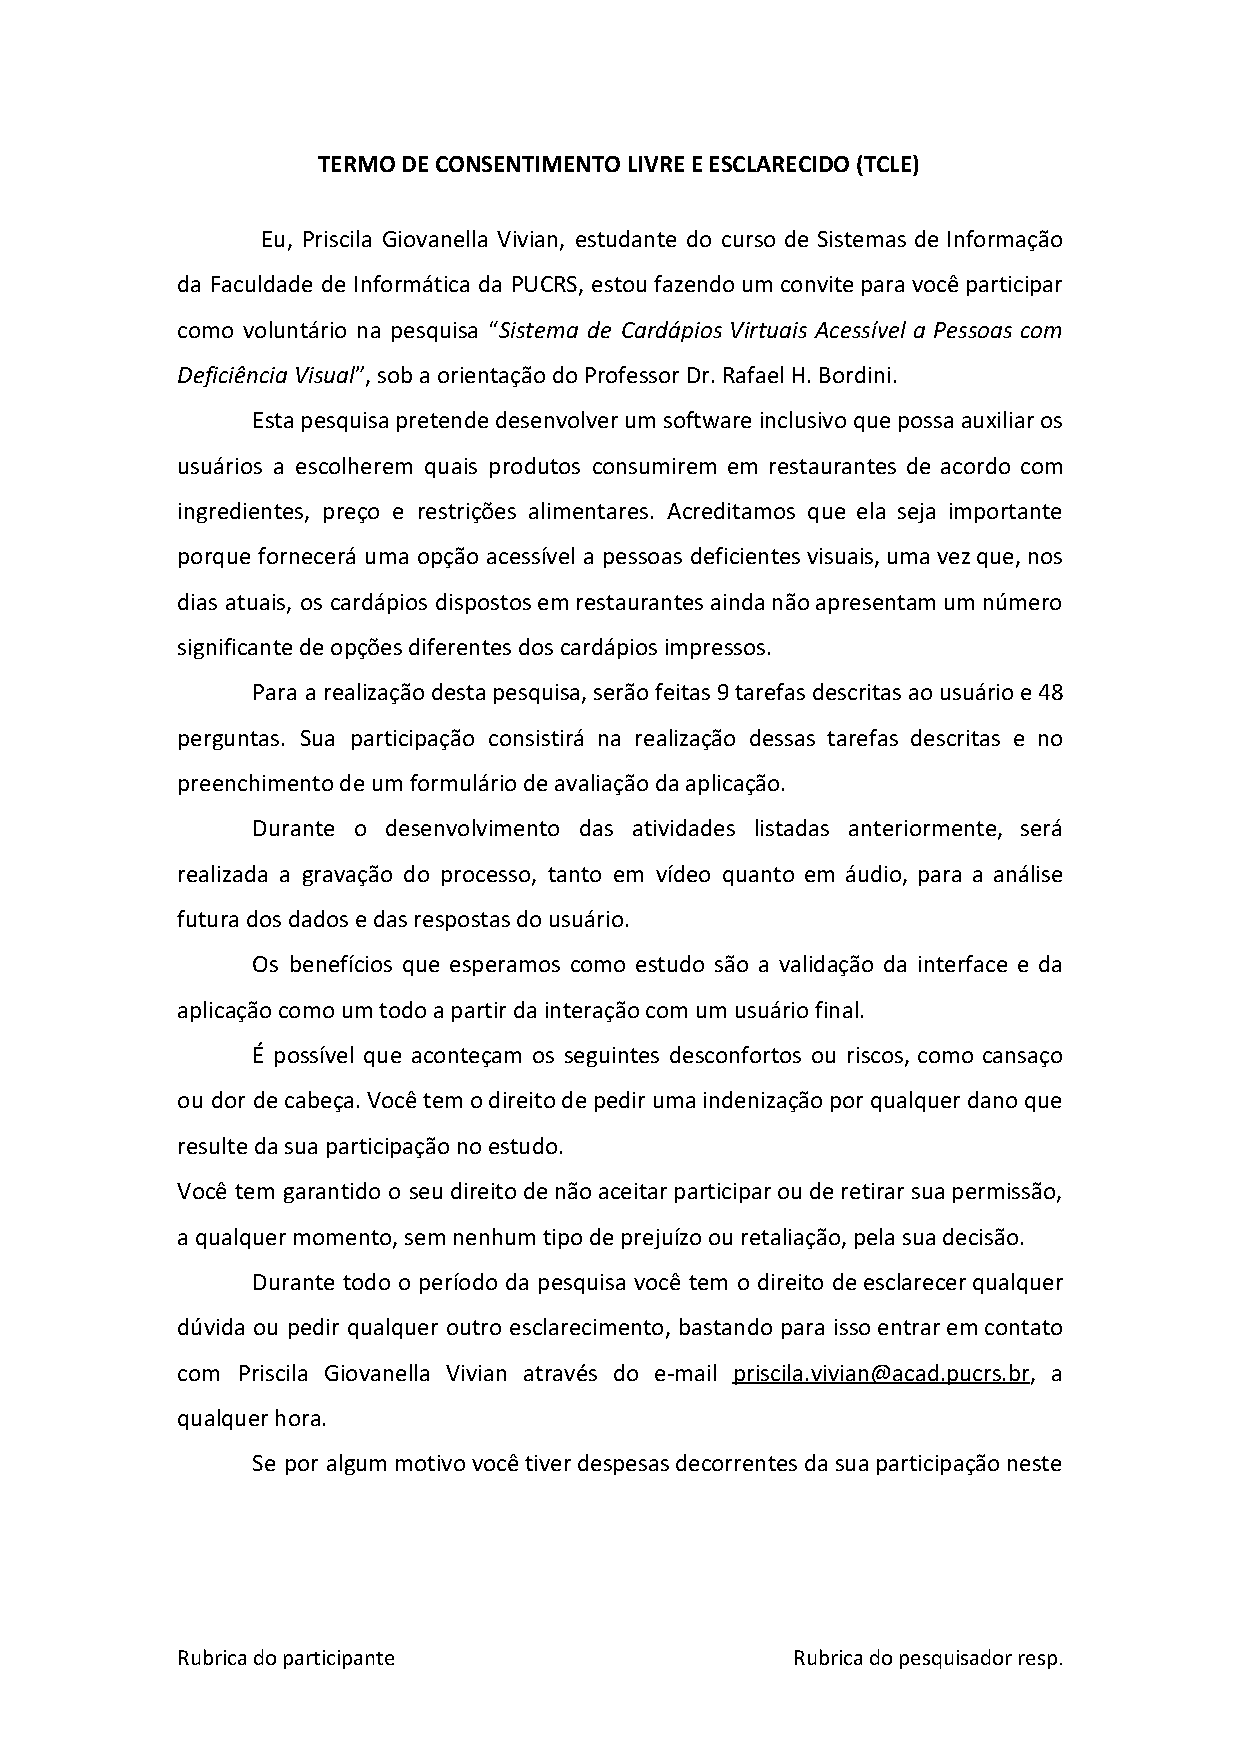
\includepdf[pages={1-},scale=1.0]{./pdf/tcle.pdf}
		
		\chapter{\label{apnd:form-1-infos}Formulários do Avaliador \#1}
		\begin{table}[!h]
			\centering
			\caption[Dados do Avaliador \#1]{\label{tab:form-1-infos}Dados do avaliador \#1}
			\tabulinesep = 0.3em
			\resizebox{\textwidth}{!}{\begin{tabu}{|l|L{18em}|}
					\cline{1-2}	
					\multicolumn{2}{|l|}{\textbf{DADOS DO AVALIADOR}} \\ \cline{1-2}	
					Avaliador & \#1 \\	\cline{1-2}	
					\multirow{10}{*}{Faixa Etária} & ( ) Abaixo de 20 anos \\ \cline{2-2}	
					& (X) 21 a 25 anos \\ \cline{2-2}	
					& ( ) 26 a 30 anos \\ \cline{2-2}
					& ( ) 31 a 35 anos \\ \cline{2-2}
					& ( ) 36 a 40 anos \\ \cline{2-2}
					& ( ) 41 a 45 anos \\ \cline{2-2}
					& ( ) 46 a 50 anos \\ \cline{2-2}
					& ( ) 51 a 55 anos \\ \cline{2-2}
					& ( ) 56 a 60 anos \\ \cline{2-2}
					& ( ) Mais de 60 anos \\ \cline{1-2}
					\multirow{2}{*}{Possui familiaridade com smartphones?} & (X) Sim \\ \cline{2-2}
					& ( ) Não \\ \cline{1-2}
					Com que frequência utiliza smartphones? & Diariamente \\ \cline{1-2}
					Com qual sistema operacional possui maior familiaridade? & Android \\ \cline{1-2}
					Modelo do smartphone utilizado & Motorola Moto G 2ª Geração \\ \cline{1-2}
					Versão do Android utilizada & Marshmallow \\ \cline{1-2}
					\multirow{2}{*}{Possui deficiência visual?} & (X) Sim \\ \cline{2-2}
					& ( ) Não \\ \cline{1-2}
					Qual o tipo de deficiência visual? & Total; glaucoma \\ \cline{1-2}
					Há quanto tempo possui esta deficiência? & Desde o nascimento \\ \cline{1-2}
					\multirow{2}{*}{Possui daltonismo?} & ( ) Sim \\ \cline{2-2}
					& (X) Não \\ \cline{1-2}
					Qual o tipo de daltonismo? & \\ \cline{1-2}
					Há quanto tempo possui esta deficiência? & \\ \cline{1-2}
					\multirow{2}{*}{Possui experiência na avaliação de aplicativos?} & (X) Sim \\ \cline{2-2}
					& ( ) Não \\ \cline{1-2}
					De quanto tempo? & 5 anos \\ \cline{1-2}
					Em que tipo de avaliação? & Avaliação de audiogames acessíveis, programação, avaliação em bioinformática, entre outros\\ \cline{1-2}
					Quantas vezes utilizou esse aplicativo? & Nenhuma \\ \cline{1-2}
					\multicolumn{2}{|l|}{\textbf{DADOS DO APLICATIVO}} \\ \cline{1-2}
					Aplicativo avaliado & Cardápio Virtual \\ \cline{1-2}
					Disponível em & 1/6/2017 \\ \cline{1-2}
					Data de avaliação & 1/6/2017 \\ \cline{1-2}
				\end{tabu}}
			\end{table}
			
			\begin{table}[!h]
				\centering
				\caption[Tarefas descritas por extenso]{\label{tab:form-1-tarefas}Lista de tarefas realizadas com os avaliadores}
				\tabulinesep = 0.5em
				\resizebox{0.75\textwidth}{!}{
					\begin{tabu}{|C{3em}|L{25em}|}
						\hline
						Índice & Tarefas \\
						\hline
						[1] & Selecionar um restaurante qualquer \\
						\hline
						[2] & Favoritar um restaurante \\
						\hline
						[3] & Desfavoritar um restaurante \\
						\hline
						[4] & Buscar um restaurante através do sistema de busca \\
						\hline
						[5] & Acessar o cardápio do restaurante Espaço 32 \\
						\hline
						[6] & Filtrar o cardápio por comidas vegetarianas, sem lactose e ordenar as informações por ordem de acesso \\
						\hline
						[7] & Verificar os ingredientes de uma "Torrada Simples" \\
						\hline
						[8] & Verificar a quantidade do produto "Pão de Queijo"\ disponível no restaurante \\
						\hline
						[9] & Voltar à tela principal após verificar as informações adicionais de um produto do cardápio \\
						\hline
					\end{tabu}}
					
				\end{table}
				
				\begin{table}[!h]
					\centering
					\caption[Tarefas do Avaliador \#1]{\label{tab:form-1-tarefas-aval}Desempenho do avaliador \#1 durante as tarefas}
					\tabulinesep = 0.5em
					\resizebox{\textwidth}{!}{\begin{tabu}{|C{3em}|L{6em}|L{6em}|C{5em}|L{6em}|L{6em}|L{10em}|}
							\cline{1-7}
							Tarefas & \multicolumn{2}{L{12em}|}{O caminho que fizeste na cabeça condiz com o caminho apresentado pelo aplicativo?} & Duração & \multicolumn{2}{L{12em}|}{Achas que conseguiria realizar a tarefa em menos tempo?} & Observação \\ \cline{1-7}
							[1] & (X) Sim & ( ) Não & 1:30 & (X) Sim & ( ) Não & Pergunta não estava muito clara\\ \cline{1-7}
							[2] & (X) Sim & ( ) Não & 0:20 & ( ) Sim & (X) Não & \\ \cline{1-7}
							[3] & (X) Sim & ( ) Não & 0:30 & ( ) Sim & (X) Não & \\ \cline{1-7}
							[4] & ( ) Sim & (X) Não & 12:00 & (X) Sim & ( ) Não & O usuário esperava que o sistema mostrasse todas as opções dos restaurantes a medida que ele fosse inserindo caracteres em sua pesquisa. O usuário também teve problemas com o teclado da versão Lollipop \\ \cline{1-7}
							[5] & (X) Sim & ( ) Não & 1:10 & ( ) Sim & (X) Não & \\ \cline{1-7}
							[6] & (X) Sim & ( ) Não & 6:00 & ( ) Sim & (X) Não & \\ \cline{1-7}
							[7] & (X) Sim & ( ) Não & 4:00 & ( ) Sim & (X) Não & O usuário gosta de explorar a tela primeiramente\\ \cline{1-7}
							[8] & (X) Sim & ( ) Não & 1:30 & ( ) Sim & (X) Não & \\ \cline{1-7}
							[9] & (X) Sim & ( ) Não & 1:50 & ( ) Sim & (X) Não & \\ \cline{1-7}
						\end{tabu}}
					\end{table}
					
					\begin{table}[!h]
						\centering
						\caption[Legenda do Questionário]{Legenda dos diferentes níveis de concordância com os quais o avaliador deve classificar cada questão do questionário}
						\tabulinesep = 0.5em
						\resizebox{0.5\textwidth}{!}{
							\begin{tabu}{|c|L{15em}|}
								\cline{1-2}
								\multicolumn{2}{|c|}{\textbf{LEGENDAS}} \\ \cline{1-2}
								1 & Discordo totalmente \\ \cline{1-2}
								2 & Discordo parcialmente \\ \cline{1-2}
								3 & Indiferente \\ \cline{1-2}
								4 & Concordo parcialmente \\ \cline{1-2}
								5 & Concordo totalmente \\ \cline{1-2}
								N/A & Não se aplica \\ \cline{1-2}
							\end{tabu}}
						\end{table}
						
						\FloatBarrier 
						\begin{center}
							\tabulinesep = 0.5em
							\begin{longtabu}{|L{25em}|c|c|c|c|c|c|}
								\caption[Questionário do Avaliador \#1]{\label{tab:form-1-questionario}Respostas do avaliador \#1 durante o preenchimento do questionário}\\
								
								\endfirsthead
								
								\multicolumn{7}{c}%
								{{\tablename\ \thetable{} -- Continuação da página anterior}} \\
								\hline
								& \textbf{1} & \textbf{2} & \textbf{3} & \textbf{4} & \textbf{5} & \textbf{N/A}\\
								\hline
								\endhead
								
								\cline{1-7}
								\textbf{1. VISIBILIDADE DO ESTADO DO SISTEMA} & \textbf{1} & \textbf{2} & \textbf{3} & \textbf{4} & \textbf{5} & \textbf{N/A} \\ \cline{1-7}
								a. O aplicativo fornece retorno (\emph{feedback}) imediato em relação ao estado do sistema. & & & & & X & \\ \cline{1-7}
								b. Os efeitos de vibração e som são facilmente identificados. & & & & & X & \\ \cline{1-7}
								c. O usuário sabe onde está no sistema.	 & & & & & X & \\ \cline{1-7}
								\textbf{2. CORRESPONDÊNCIA ENTRE O SISTEMA E O MUNDO REAL} & \textbf{1} & \textbf{2} & \textbf{3} & \textbf{4} & \textbf{5} & \textbf{N/A} \\ \cline{1-7}
								a. Os conceitos relacionados a restaurantes e alimentação utilizados no aplicativo são compreensíveis. & & & & & X & \\ \cline{1-7}
								b. No cardápio, o agrupamento de produtos por categorias é compreensível. & & & & & X & \\ \cline{1-7}
								\textbf{3. CONTROLE E LIBERDADE DO USUÁRIO} & \textbf{1} & \textbf{2} & \textbf{3} & \textbf{4} & \textbf{5} & \textbf{N/A} \\ \cline{1-7}
								a. O usuário sente que está no controle. & & & & & X & \\ \cline{1-7}
								b. É fácil voltar a um ponto anterior no aplicativo. & & & & & X & \\ \cline{1-7}
								c. É fácil retornar à tela principal do aplicativo. & & & & & X & \\ \cline{1-7}
								\textbf{4. CONSISTÊNCIA E PADRONIZAÇÃO} & \textbf{1} & \textbf{2} & \textbf{3} & \textbf{4} & \textbf{5} & \textbf{N/A} \\ \cline{1-7}
								a. Há coerência entre as opções do aplicativo e o que elas fazem. & & & & & X & \\ \cline{1-7}
								b. A interface sonora é consistente. & & & & & X & \\ \cline{1-7}
								c. A interface gráfica é consistente. & & & & & & X \\ \cline{1-7}
								d. Os recursos de vibração são consistentes. & & & & & X & \\ \cline{1-7}
								e. O aplicativo apresenta uma padrão em sua interface. & & & & & X & \\ \cline{1-7}
								f. Os nomes das funções e objetos de interação são familiares para o usuário. & & & & & X & \\ \cline{1-7}
								g. As telas e caixas de diálogo possuem títulos claros. & & & & & X & \\ \cline{1-7}
								\textbf{5. PREVENÇÃO DE ERROS} & \textbf{1} & \textbf{2} & \textbf{3} & \textbf{4} & \textbf{5} & \textbf{N/A} \\ \cline{1-7}
								a. O Aplicativo evita que o usuário cometa erros, por exemplo, habilitando somente opções que possam ser utilizadas. & & & & & X & \\ \cline{1-7}
								\textbf{6. RECONHECIMENTO AO INVÉS DE MEMORIZAÇÃO} & \textbf{1} & \textbf{2} & \textbf{3} & \textbf{4} & \textbf{5} & \textbf{N/A} \\ \cline{1-7}
								a. O  menu é de uso intuitivo. & & & & & X & \\ \cline{1-7}
								b. Os controles são intuitivos. & & & & & X & \\ \cline{1-7}
								c. O aplicativo não exige o aprendizado intensivo ou leitura de vasta documentação para ser utilizado. & & & & & X & \\ \cline{1-7}
								d. As informações apresentadas são fáceis de entender. & & & & & X & \\ \cline{1-7}
								\textbf{7. FLEXIBILIDADE E EFICIÊNCIA DE USO} & \textbf{1} & \textbf{2} & \textbf{3} & \textbf{4} & \textbf{5} & \textbf{N/A} \\ \cline{1-7}
								a. O aplicativo permite que o usuário selecione o restaurante conforme suas necessidades. & & & & & X & \\ \cline{1-7}
								b. Depois que o usuário aprende a utilizar o aplicativo, é mais produtivo consultar os restaurantes antes de ir fisicamente aos mesmos. & & & & & X & \\ \cline{1-7}
								c. O usuário consegue alterar suas preferências relacionadas à alimentação. & & & & & X & \\ \cline{1-7}
								d. O aplicativo exige pouca carga de trabalho do usuário. & & & & & X & \\ \cline{1-7}
								e. Com poucas ações, é possível selecionar filtros e buscar restaurantes. & & & & & X & \\ \cline{1-7}
								f. O aplicativo distribui as opções em função de sua frequência de utilização ou de sua relevância no contexto.	& & & & & X & \\ \cline{1-7}
								g. O aplicativo fornece um conjunto adequado de opções para que o usuário selecione restaurantes. & & & & & X & \\ \cline{1-7}
								\textbf{8. PROJETO ESTÉTICO E MINIMALISTA} & \textbf{1} & \textbf{2} & \textbf{3} & \textbf{4} & \textbf{5} & \textbf{N/A} \\ \cline{1-7}
								a. O aplicativo fornece um conjunto adequado de opções por tela, não saturando o usuário com muitas informações. & & & & & X & \\ \cline{1-7}
								b. A navegação segue uma lógica. & & & & & X & \\ \cline{1-7}
								c. As informações apresentadas ao usuário são relevantes. & & & & & X & \\ \cline{1-7}
								\textbf{9. RECONHECIMENTO, DIAGNÓSTICO E RECUPERAÇÃO DE ERROS} & \textbf{1} & \textbf{2} & \textbf{3} & \textbf{4} & \textbf{5} & \textbf{N/A} \\ \cline{1-7}
								a. É fácil saber quando ocorre um erro.	& & & & X & & \\ \cline{1-7}
								b. É fácil saber porque ocorreu um erro. & & & & & X & \\ \cline{1-7}
								c. O aplicativo informa como sair de um estado indesejado. & & & & & X & \\ \cline{1-7}
								\textbf{10. AJUDA E DOCUMENTAÇÃO} & \textbf{1} & \textbf{2} & \textbf{3} & \textbf{4} & \textbf{5} & \textbf{N/A} \\ \cline{1-7}
								a. O aplicativo fornece ajuda ao usuário para facilitar o entendimento do sistema. & & & X & & & \\ \cline{1-7}
								\textbf{11. ACESSIBILIDADE} & \textbf{1} & \textbf{2} & \textbf{3} & \textbf{4} & \textbf{5} & \textbf{N/A} \\ \cline{1-7}
								a. Caso tenha sido necessário, foi possível redimensionar os elementos da tela do aplicativo. & & & & & & X \\ \cline{1-7}
								b. O tamanho e espaçamento dos elementos da tela permite fácil seleção dos ícones e demais opções do aplicativo. & & & & & & X \\ \cline{1-7}
								c. O aplicativo se adapta a orientação do dispositivo e pode ser utilizado com o \emph{smartphone} tanto na vertical quanto na horizontal. & & & & & X & \\ \cline{1-7}
								d. Os elementos da tela seguem uma organização lógica. & & & & & X & \\ \cline{1-7}
								e. É fácil de identificar que elementos da tela podem ser acionados (ícones, botões, links, etc.) e quais não. & & & & & X & \\ \cline{1-7}
								f. É fácil de adicionar as informações requisitadas pelo aplicativo (quando existem opções finitas, o aplicativo oferece um menu com opções em vez de obrigar o usuário a digitar todas as vezes). & & & & & X & \\ \cline{1-7}
								g. O aplicativo é compatível com as ferramentas de \emph{text-to-speech}. & & & & & X & \\ \cline{1-7}
								h. O aplicativo é compatível com as funções do TalkBack. & & & & & X & \\ \cline{1-7}
								i. É possível realizar todas as funções do aplicativo com facilidade através da utilização do TalkBack.	& & & & & X & \\ \cline{1-7}
								j. Utilizando-se TalkBack (ou \emph{text-to-speech}) é fácil entender a função dos elementos apresentados na tela do aplicativo. & & & & & X & \\ \cline{1-7}
								l. O conteúdo do aplicativo é completamente legível (não mistura de idiomas, não apresenta abreviações sem explicação ou ícones sem informação textual). & & & & & X & \\ \cline{1-7}
								m. O aplicativo oferece alternativas para a diferenciação dos elementos da tela além de diferentes colorações. & & & & & & X \\ \cline{1-7}
								n. O aplicativo é compatível com a função de correção de cores do \emph{smartphone}. & & & & & & X \\ \cline{1-7}
								o. O aplicativo é compatível com a função de inversão de cores do \emph{smartphone}. & & & & & & X \\ \cline{1-7}
							\end{longtabu}
						\end{center}
						
						\begin{table}[!h]
							\centering
							\caption[Questionário do Avaliador \#1 -- Sumarizado]{Sumarização das respostas do avaliador \#1}
							\tabulinesep = 0.5em
							\resizebox{0.8\textwidth}{!}{
								\begin{tabu}{|C{1.5em}|C{1.5em}|C{1.5em}|C{1.5em}|C{1.5em}|c|c|c|c|}
									\cline{1-9}
									\multicolumn{9}{|l|}{\textbf{1. VISIBILIDADE DO ESTADO DO SISTEMA}} \\ \cline{1-9}
									\textbf{1} & \textbf{2} & \textbf{3} & \textbf{4} & \textbf{5} & \textbf{N/A} & \textbf{TOTAL} & \textbf{QTD. VÁLIDA} & \textbf{MÉDIA} \\ \cline{1-9}
									0 & 0 & 0 & 0 & 3 & 0 & 15 & 3 & 5.0 \\ \cline{1-9}
									\multicolumn{9}{|l|}{\textbf{2. CORRESPONDÊNCIA ENTRE O SISTEMA E O MUNDO REAL}} \\ \cline{1-9}
									\textbf{1} & \textbf{2} & \textbf{3} & \textbf{4} & \textbf{5} & \textbf{N/A} & \textbf{TOTAL} & \textbf{QTD. VÁLIDA} & \textbf{MÉDIA} \\ \cline{1-9}
									0 & 0 & 0 & 0 & 2 & 0 & 10 & 2 & 5.0 \\ \cline{1-9}
									\multicolumn{9}{|l|}{\textbf{3. CONTROLE E LIBERDADE DO USUÁRIO}} \\ \cline{1-9}
									\textbf{1} & \textbf{2} & \textbf{3} & \textbf{4} & \textbf{5} & \textbf{N/A} & \textbf{TOTAL} & \textbf{QTD. VÁLIDA} & \textbf{MÉDIA} \\ \cline{1-9}
									0 & 0 & 0 & 0 & 3 & 0 & 15 & 3 & 5.0 \\ \cline{1-9}
									\multicolumn{9}{|l|}{\textbf{4. CONSISTÊNCIA E PADRONIZAÇÃO}} \\ \cline{1-9}
									\textbf{1} & \textbf{2} & \textbf{3} & \textbf{4} & \textbf{5} & \textbf{N/A} & \textbf{TOTAL} & \textbf{QTD. VÁLIDA} & \textbf{MÉDIA} \\ \cline{1-9}
									0 & 0 & 0 & 0 & 6 & 1 & 30 & 6 & 5.0 \\ \cline{1-9}
									\multicolumn{9}{|l|}{\textbf{5. PREVENÇÃO DE ERROS}} \\ \cline{1-9}
									\textbf{1} & \textbf{2} & \textbf{3} & \textbf{4} & \textbf{5} & \textbf{N/A} & \textbf{TOTAL} & \textbf{QTD. VÁLIDA} & \textbf{MÉDIA} \\ \cline{1-9}
									0 & 0 & 0 & 0 & 1 & 0 & 5 & 1 & 5.0 \\ \cline{1-9}
									\multicolumn{9}{|l|}{\textbf{6. RECONHECIMENTO AO INVÉS DE MEMORIZAÇÃO}} \\ \cline{1-9}
									\textbf{1} & \textbf{2} & \textbf{3} & \textbf{4} & \textbf{5} & \textbf{N/A} & \textbf{TOTAL} & \textbf{QTD. VÁLIDA} & \textbf{MÉDIA} \\ \cline{1-9}
									0 & 0 & 0 & 0 & 4 & 0 & 20 & 4 & 5.0 \\ \cline{1-9}
									\multicolumn{9}{|l|}{\textbf{7. FLEXIBILIDADE E EFICIÊNCIA DE USO}} \\ \cline{1-9}
									\textbf{1} & \textbf{2} & \textbf{3} & \textbf{4} & \textbf{5} & \textbf{N/A} & \textbf{TOTAL} & \textbf{QTD. VÁLIDA} & \textbf{MÉDIA} \\ \cline{1-9}
									0 & 0 & 0 & 0 & 7 & 0 & 35 & 7 & 5.0 \\ \cline{1-9}
									\multicolumn{9}{|l|}{\textbf{8. PROJETO ESTÉTICO E MINIMALISTA}} \\ \cline{1-9}
									\textbf{1} & \textbf{2} & \textbf{3} & \textbf{4} & \textbf{5} & \textbf{N/A} & \textbf{TOTAL} & \textbf{QTD. VÁLIDA} & \textbf{MÉDIA} \\ \cline{1-9}
									0 & 0 & 0 & 0 & 3 & 0 & 15 & 3 & 5.0 \\ \cline{1-9}
									\multicolumn{9}{|l|}{\textbf{9. RECONHECIMENTO, DIAGNÓSTICO E RECUPERAÇÃO DE ERROS}} \\ \cline{1-9}
									\textbf{1} & \textbf{2} & \textbf{3} & \textbf{4} & \textbf{5} & \textbf{N/A} & \textbf{TOTAL} & \textbf{QTD. VÁLIDA} & \textbf{MÉDIA} \\ \cline{1-9}
									0 & 0 & 0 & 1 & 2 & 0 & 14 & 3 & 4.7 \\ \cline{1-9}
									\multicolumn{9}{|l|}{\textbf{10. AJUDA E DOCUMENTAÇÃO}} \\ \cline{1-9}
									\textbf{1} & \textbf{2} & \textbf{3} & \textbf{4} & \textbf{5} & \textbf{N/A} & \textbf{TOTAL} & \textbf{QTD. VÁLIDA} & \textbf{MÉDIA} \\ \cline{1-9}
									0 & 0 & 1 & 0 & 0 & 0 & 3 & 1 & 3.0 \\ \cline{1-9}
									\multicolumn{9}{|l|}{\textbf{11. ACESSIBILIDADE}} \\ \cline{1-9}
									\textbf{1} & \textbf{2} & \textbf{3} & \textbf{4} & \textbf{5} & \textbf{N/A} & \textbf{TOTAL} & \textbf{QTD. VÁLIDA} & \textbf{MÉDIA} \\ \cline{1-9}
									0 & 0 & 0 & 0 & 9 & 5 & 45 & 9 & 5.0 \\ \cline{1-9}
								\end{tabu}}
							\end{table}
							
							\chapter{\label{apnd:form-2-infos}Formulários do Avaliador \#2}
							\begin{table}[!h]
								\centering
								\caption[Dados do Avaliador \#2]{\label{tab:form-2-infos}Dados do avaliador \#2}
								\tabulinesep = 0.3em
								\resizebox{\textwidth}{!}{\begin{tabu}{|l|L{18em}|}
										\cline{1-2}	
										\multicolumn{2}{|l|}{\textbf{DADOS DO AVALIADOR}} \\ \cline{1-2}	
										Avaliador & \#2 \\	\cline{1-2}	
										\multirow{10}{*}{Faixa Etária} & ( ) Abaixo de 20 anos \\ \cline{2-2}	
										& () 21 a 25 anos \\ \cline{2-2}	
										& ( ) 26 a 30 anos \\ \cline{2-2}
										& ( ) 31 a 35 anos \\ \cline{2-2}
										& ( ) 36 a 40 anos \\ \cline{2-2}
										& ( ) 41 a 45 anos \\ \cline{2-2}
										& (X) 46 a 50 anos \\ \cline{2-2}
										& ( ) 51 a 55 anos \\ \cline{2-2}
										& ( ) 56 a 60 anos \\ \cline{2-2}
										& ( ) Mais de 60 anos \\ \cline{1-2}
										\multirow{2}{*}{Possui familiaridade com smartphones?} & (X) Sim \\ \cline{2-2}
										& ( ) Não \\ \cline{1-2}
										Com que frequência utiliza smartphones? & Diariamente \\ \cline{1-2}
										Com qual sistema operacional possui maior familiaridade? & Android \\ \cline{1-2}
										Modelo do smartphone utilizado & Samsung Galaxy Pocket Neo Gt \\ \cline{1-2}
										Versão do Android utilizada & Jelly Bean \\ \cline{1-2}
										\multirow{2}{*}{Possui deficiência visual?} & ( ) Sim \\ \cline{2-2}
										& (X) Não \\ \cline{1-2}
										Qual o tipo de deficiência visual? & \\ \cline{1-2}
										Há quanto tempo possui esta deficiência? & \\ \cline{1-2}
										\multirow{2}{*}{Possui daltonismo?} & ( ) Sim \\ \cline{2-2}
										& (X) Não \\ \cline{1-2}
										Qual o tipo de daltonismo? & \\ \cline{1-2}
										Há quanto tempo possui esta deficiência? & \\ \cline{1-2}
										\multirow{2}{*}{Possui experiência na avaliação de aplicativos?} & ( ) Sim \\ \cline{2-2}
										& (X) Não \\ \cline{1-2}
										De quanto tempo? & \\ \cline{1-2}
										Em que tipo de avaliação? & \\ \cline{1-2}
										Quantas vezes utilizou esse aplicativo? & Nenhuma \\ \cline{1-2}
										\multicolumn{2}{|l|}{\textbf{DADOS DO APLICATIVO}} \\ \cline{1-2}
										Aplicativo avaliado & Cardápio Virtual \\ \cline{1-2}
										Disponível em & 6/6/2017 \\ \cline{1-2}
										Data de avaliação & 6/6/2017 \\ \cline{1-2}
									\end{tabu}}
								\end{table}
								
								\begin{table}[!h]
									\centering
									\caption[Tarefas descritas por extenso]{\label{tab:form-2-tarefas}Lista de tarefas realizadas com os avaliadores}
									\tabulinesep = 0.5em
									\resizebox{0.75\textwidth}{!}{
										\begin{tabu}{|C{3em}|L{25em}|}
											\hline
											Índice & Tarefas \\
											\hline
											[1] & Selecionar um restaurante qualquer \\
											\hline
											[2] & Favoritar um restaurante \\
											\hline
											[3] & Desfavoritar um restaurante \\
											\hline
											[4] & Buscar um restaurante através do sistema de busca \\
											\hline
											[5] & Acessar o cardápio do restaurante Espaço 32 \\
											\hline
											[6] & Filtrar o cardápio por comidas vegetarianas, sem lactose e ordenar as informações por ordem de acesso \\
											\hline
											[7] & Verificar os ingredientes de uma "Torrada Simples" \\
											\hline
											[8] & Verificar a quantidade do produto "Pão de Queijo"\ disponível no restaurante \\
											\hline
											[9] & Voltar à tela principal após verificar as informações adicionais de um produto do cardápio \\
											\hline
										\end{tabu}}
										
									\end{table}
									
									\begin{table}[!h]
										\centering
										\caption[Tarefas do Avaliador \#2]{\label{tab:form-2-tarefas-aval}Desempenho do avaliador \#2 durante as tarefas}
										\tabulinesep = 0.5em
										\resizebox{\textwidth}{!}{\begin{tabu}{|C{3em}|L{6em}|L{6em}|C{5em}|L{6em}|L{6em}|L{10em}|}
												\cline{1-7}
												Tarefas & \multicolumn{2}{L{12em}|}{O caminho que fizeste na cabeça condiz com o caminho apresentado pelo aplicativo?} & Duração & \multicolumn{2}{L{12em}|}{Achas que conseguiria realizar a tarefa em menos tempo?} & Observação \\ \cline{1-7}
												[1] & (X) Sim & ( ) Não & 0:06 & ( ) Sim & (X) Não & \\ \cline{1-7}
												[2] & (X) Sim & ( ) Não & 0:08 & ( ) Sim & (X) Não & \\ \cline{1-7}
												[3] & (X) Sim & ( ) Não & 0:05 & ( ) Sim & (X) Não & \\ \cline{1-7}
												[4] & (X) Sim & ( ) Não & 0:20 & ( ) Sim & (X) Não & \\ \cline{1-7}
												[5] & (X) Sim & ( ) Não & 0:05 & ( ) Sim & (X) Não & \\ \cline{1-7}
												[6] & (X) Sim & ( ) Não & 0:18 & ( ) Sim & (X) Não & \\ \cline{1-7}
												[7] & (X) Sim & ( ) Não & 0:34 & ( ) Sim & (X) Não & O nome "categoria refeição"\ não deixa claro o que a categoria oferece \\ \cline{1-7}
												[8] & (X) Sim & ( ) Não & 0:25 & ( ) Sim & (X) Não & \\ \cline{1-7}
												[9] & (X) Sim & ( ) Não & 0:07 & (X) Sim & ( ) Não & Se tivesse um botão de "home", seria mais rápido \\ \cline{1-7}
											\end{tabu}}
										\end{table}
										
										\begin{table}[!h]
											\centering
											\caption[Legenda do Questionário]{\label{tab:form-2-legenda}Legenda dos diferentes níveis de concordância com os quais o avaliador deve classificar cada questão do questionário}
											\tabulinesep = 0.5em
											\resizebox{0.5\textwidth}{!}{
												\begin{tabu}{|c|L{15em}|}
													\cline{1-2}
													\multicolumn{2}{|c|}{\textbf{LEGENDAS}} \\ \cline{1-2}
													1 & Discordo totalmente \\ \cline{1-2}
													2 & Discordo parcialmente \\ \cline{1-2}
													3 & Indiferente \\ \cline{1-2}
													4 & Concordo parcialmente \\ \cline{1-2}
													5 & Concordo totalmente \\ \cline{1-2}
													N/A & Não se aplica \\ \cline{1-2}
												\end{tabu}}
											\end{table}
											
											\FloatBarrier 
											\begin{center}
												\tabulinesep = 0.5em
												\begin{longtabu}{|L{25em}|c|c|c|c|c|c|}
													\caption[Questionário do Avaliador \#2]{\label{tab:form-2-questionario}Respostas do avaliador \#2 durante o preenchimento do questionário}\\
													
													\endfirsthead
													
													\multicolumn{7}{c}%
													{{\tablename\ \thetable{} -- Continuação da página anterior}} \\
													\hline
													& \textbf{1} & \textbf{2} & \textbf{3} & \textbf{4} & \textbf{5} & \textbf{N/A}\\
													\hline
													\endhead
													\cline{1-7}
													\textbf{1. VISIBILIDADE DO ESTADO DO SISTEMA} & \textbf{1} & \textbf{2} & \textbf{3} & \textbf{4} & \textbf{5} & \textbf{N/A} \\ \cline{1-7}
													a. O aplicativo fornece retorno (\emph{feedback}) imediato em relação ao estado do sistema. & & & & & X & \\ \cline{1-7}
													b. Os efeitos de vibração e som são facilmente identificados. & & & & & & X \\ \cline{1-7}
													c. O usuário sabe onde está no sistema.	 & & & & & X & \\ \cline{1-7}
													\textbf{2. CORRESPONDÊNCIA ENTRE O SISTEMA E O MUNDO REAL} & \textbf{1} & \textbf{2} & \textbf{3} & \textbf{4} & \textbf{5} & \textbf{N/A} \\ \cline{1-7}
													a. Os conceitos relacionados a restaurantes e alimentação utilizados no aplicativo são compreensíveis. & & & & & X & \\ \cline{1-7}
													b. No cardápio, o agrupamento de produtos por categorias é compreensível. & & & & X & & \\ \cline{1-7}
													\textbf{3. CONTROLE E LIBERDADE DO USUÁRIO} & \textbf{1} & \textbf{2} & \textbf{3} & \textbf{4} & \textbf{5} & \textbf{N/A} \\ \cline{1-7}
													a. O usuário sente que está no controle. & & & & & X & \\ \cline{1-7}
													b. É fácil voltar a um ponto anterior no aplicativo. & & & & & X & \\ \cline{1-7}
													c. É fácil retornar à tela principal do aplicativo. & & & & X & & \\ \cline{1-7}
													\textbf{4. CONSISTÊNCIA E PADRONIZAÇÃO} & \textbf{1} & \textbf{2} & \textbf{3} & \textbf{4} & \textbf{5} & \textbf{N/A} \\ \cline{1-7}
													a. Há coerência entre as opções do aplicativo e o que elas fazem. & & & & & X & \\ \cline{1-7}
													b. A interface sonora é consistente. & & & & & & X \\ \cline{1-7}
													c. A interface gráfica é consistente. & & & & & X & \\ \cline{1-7}
													d. Os recursos de vibração são consistentes. & & & & & & X \\ \cline{1-7}
													e. O aplicativo apresenta uma padrão em sua interface. & & & & & X & \\ \cline{1-7}
													f. Os nomes das funções e objetos de interação são familiares para o usuário. & & & & & X & \\ \cline{1-7}
													g. As telas e caixas de diálogo possuem títulos claros. & & & & & X & \\ \cline{1-7}
													\textbf{5. PREVENÇÃO DE ERROS} & \textbf{1} & \textbf{2} & \textbf{3} & \textbf{4} & \textbf{5} & \textbf{N/A} \\ \cline{1-7}
													a. O Aplicativo evita que o usuário cometa erros, por exemplo, habilitando somente opções que possam ser utilizadas. & & & & & & X \\ \cline{1-7}
													\textbf{6. RECONHECIMENTO AO INVÉS DE MEMORIZAÇÃO} & \textbf{1} & \textbf{2} & \textbf{3} & \textbf{4} & \textbf{5} & \textbf{N/A} \\ \cline{1-7}
													a. O  menu é de uso intuitivo. & & & & & X & \\ \cline{1-7}
													b. Os controles são intuitivos. & & & & & X & \\ \cline{1-7}
													c. O aplicativo não exige o aprendizado intensivo ou leitura de vasta documentação para ser utilizado. & & & & & X & \\ \cline{1-7}
													d. As informações apresentadas são fáceis de entender. & & & & & X & \\ \cline{1-7}
													\textbf{7. FLEXIBILIDADE E EFICIÊNCIA DE USO} & \textbf{1} & \textbf{2} & \textbf{3} & \textbf{4} & \textbf{5} & \textbf{N/A} \\ \cline{1-7}
													a. O aplicativo permite que o usuário selecione o restaurante conforme suas necessidades. & & & & & X & \\ \cline{1-7}
													b. Depois que o usuário aprende a utilizar o aplicativo, é mais produtivo consultar os restaurantes antes de ir fisicamente aos mesmos. & & & & & X & \\ \cline{1-7}
													c. O usuário consegue alterar suas preferências relacionadas à alimentação. & & & & & X & \\ \cline{1-7}
													d. O aplicativo exige pouca carga de trabalho do usuário. & & & & & X & \\ \cline{1-7}
													e. Com poucas ações, é possível selecionar filtros e buscar restaurantes. & & & & & X & \\ \cline{1-7}
													f. O aplicativo distribui as opções em função de sua frequência de utilização ou de sua relevância no contexto.	& & & & & X & \\ \cline{1-7}
													g. O aplicativo fornece um conjunto adequado de opções para que o usuário selecione restaurantes. & & & & & X & \\ \cline{1-7}
													\textbf{8. PROJETO ESTÉTICO E MINIMALISTA} & \textbf{1} & \textbf{2} & \textbf{3} & \textbf{4} & \textbf{5} & \textbf{N/A} \\ \cline{1-7}
													a. O aplicativo fornece um conjunto adequado de opções por tela, não saturando o usuário com muitas informações. & & & & & X & \\ \cline{1-7}
													b. A navegação segue uma lógica. & & & & & X & \\ \cline{1-7}
													c. As informações apresentadas ao usuário são relevantes. & & & & & X & \\ \cline{1-7}
													\textbf{9. RECONHECIMENTO, DIAGNÓSTICO E RECUPERAÇÃO DE ERROS} & \textbf{1} & \textbf{2} & \textbf{3} & \textbf{4} & \textbf{5} & \textbf{N/A} \\ \cline{1-7}
													a. É fácil saber quando ocorre um erro.	& & & & & X & \\ \cline{1-7}
													b. É fácil saber porque ocorreu um erro. & X & & & & & \\ \cline{1-7}
													c. O aplicativo informa como sair de um estado indesejado. & & & X & & & \\ \cline{1-7}
													\textbf{10. AJUDA E DOCUMENTAÇÃO} & \textbf{1} & \textbf{2} & \textbf{3} & \textbf{4} & \textbf{5} & \textbf{N/A} \\ \cline{1-7}
													a. O aplicativo fornece ajuda ao usuário para facilitar o entendimento do sistema. & & & & X & & \\ \cline{1-7}
													\textbf{11. ACESSIBILIDADE} & \textbf{1} & \textbf{2} & \textbf{3} & \textbf{4} & \textbf{5} & \textbf{N/A} \\ \cline{1-7}
													a. Caso tenha sido necessário, foi possível redimensionar os elementos da tela do aplicativo. & & & & & X & \\ \cline{1-7}
													b. O tamanho e espaçamento dos elementos da tela permite fácil seleção dos ícones e demais opções do aplicativo. & & & & & X & \\ \cline{1-7}
													c. O aplicativo se adapta a orientação do dispositivo e pode ser utilizado com o \emph{smartphone} tanto na vertical quanto na horizontal. & & & & & X & \\ \cline{1-7}
													d. Os elementos da tela seguem uma organização lógica. & & & & & X & \\ \cline{1-7}
													e. É fácil de identificar que elementos da tela podem ser acionados (ícones, botões, links, etc.) e quais não. & & & & & X & \\ \cline{1-7}
													f. É fácil de adicionar as informações requisitadas pelo aplicativo (quando existem opções finitas, o aplicativo oferece um menu com opções em vez de obrigar o usuário a digitar todas as vezes). & & & & & X & \\ \cline{1-7}
													g. O aplicativo é compatível com as ferramentas de \emph{text-to-speech}. & & & & & & X \\ \cline{1-7}
													h. O aplicativo é compatível com as funções do TalkBack. & & & & & & X \\ \cline{1-7}
													i. É possível realizar todas as funções do aplicativo com facilidade através da utilização do TalkBack.	& & & & & & X \\ \cline{1-7}
													j. Utilizando-se TalkBack (ou \emph{text-to-speech}) é fácil entender a função dos elementos apresentados na tela do aplicativo. & & & & & & X \\ \cline{1-7}
													l. O conteúdo do aplicativo é completamente legível (não mistura de idiomas, não apresenta abreviações sem explicação ou ícones sem informação textual). & & & & & X & \\ \cline{1-7}
													m. O aplicativo oferece alternativas para a diferenciação dos elementos da tela além de diferentes colorações. & & & & & X & \\ \cline{1-7}
													n. O aplicativo é compatível com a função de correção de cores do \emph{smartphone}. & & & & & X & \\ \cline{1-7}
													o. O aplicativo é compatível com a função de inversão de cores do \emph{smartphone}. & & & & & X & \\ \cline{1-7}
												\end{longtabu}
											\end{center}
											
											\begin{table}[!h]
												\centering
												\caption[Questionário do Avaliador \#2 -- Sumarizado]{\label{tab:form-2-sumar}Sumarização das respostas do avaliador \#2}
												\tabulinesep = 0.5em
												\resizebox{0.8\textwidth}{!}{
													\begin{tabu}{|C{1.5em}|C{1.5em}|C{1.5em}|C{1.5em}|C{1.5em}|c|c|c|c|}
														\cline{1-9}
														\multicolumn{9}{|l|}{\textbf{1. VISIBILIDADE DO ESTADO DO SISTEMA}} \\ \cline{1-9}
														\textbf{1} & \textbf{2} & \textbf{3} & \textbf{4} & \textbf{5} & \textbf{N/A} & \textbf{TOTAL} & \textbf{QTD. VÁLIDA} & \textbf{MÉDIA} \\ \cline{1-9}
														0 & 0 & 0 & 0 & 2 & 1 & 10 & 2 & 5.0 \\ \cline{1-9}
														\multicolumn{9}{|l|}{\textbf{2. CORRESPONDÊNCIA ENTRE O SISTEMA E O MUNDO REAL}} \\ \cline{1-9}
														\textbf{1} & \textbf{2} & \textbf{3} & \textbf{4} & \textbf{5} & \textbf{N/A} & \textbf{TOTAL} & \textbf{QTD. VÁLIDA} & \textbf{MÉDIA} \\ \cline{1-9}
														0 & 0 & 0 & 1 & 1 & 0 & 9 & 2 & 4.5 \\ \cline{1-9}
														\multicolumn{9}{|l|}{\textbf{3. CONTROLE E LIBERDADE DO USUÁRIO}} \\ \cline{1-9}
														\textbf{1} & \textbf{2} & \textbf{3} & \textbf{4} & \textbf{5} & \textbf{N/A} & \textbf{TOTAL} & \textbf{QTD. VÁLIDA} & \textbf{MÉDIA} \\ \cline{1-9}
														0 & 0 & 0 & 1 & 2 & 0 & 14 & 3 & 4.7 \\ \cline{1-9}
														\multicolumn{9}{|l|}{\textbf{4. CONSISTÊNCIA E PADRONIZAÇÃO}} \\ \cline{1-9}
														\textbf{1} & \textbf{2} & \textbf{3} & \textbf{4} & \textbf{5} & \textbf{N/A} & \textbf{TOTAL} & \textbf{QTD. VÁLIDA} & \textbf{MÉDIA} \\ \cline{1-9}
														0 & 0 & 0 & 0 & 5 & 2 & 25 & 5 & 5.0 \\ \cline{1-9}
														\multicolumn{9}{|l|}{\textbf{5. PREVENÇÃO DE ERROS}} \\ \cline{1-9}
														\textbf{1} & \textbf{2} & \textbf{3} & \textbf{4} & \textbf{5} & \textbf{N/A} & \textbf{TOTAL} & \textbf{QTD. VÁLIDA} & \textbf{MÉDIA} \\ \cline{1-9}
														0 & 0 & 0 & 0 & 0 & 1 & 0 & 0 &  \\ \cline{1-9}
														\multicolumn{9}{|l|}{\textbf{6. RECONHECIMENTO AO INVÉS DE MEMORIZAÇÃO}} \\ \cline{1-9}
														\textbf{1} & \textbf{2} & \textbf{3} & \textbf{4} & \textbf{5} & \textbf{N/A} & \textbf{TOTAL} & \textbf{QTD. VÁLIDA} & \textbf{MÉDIA} \\ \cline{1-9}
														0 & 0 & 0 & 0 & 4 & 0 & 20 & 4 & 5.0 \\ \cline{1-9}
														\multicolumn{9}{|l|}{\textbf{7. FLEXIBILIDADE E EFICIÊNCIA DE USO}} \\ \cline{1-9}
														\textbf{1} & \textbf{2} & \textbf{3} & \textbf{4} & \textbf{5} & \textbf{N/A} & \textbf{TOTAL} & \textbf{QTD. VÁLIDA} & \textbf{MÉDIA} \\ \cline{1-9}
														0 & 0 & 0 & 0 & 7 & 0 & 35 & 7 & 5.0 \\ \cline{1-9}
														\multicolumn{9}{|l|}{\textbf{8. PROJETO ESTÉTICO E MINIMALISTA}} \\ \cline{1-9}
														\textbf{1} & \textbf{2} & \textbf{3} & \textbf{4} & \textbf{5} & \textbf{N/A} & \textbf{TOTAL} & \textbf{QTD. VÁLIDA} & \textbf{MÉDIA} \\ \cline{1-9}
														0 & 0 & 0 & 0 & 3 & 0 & 15 & 3 & 5.0 \\ \cline{1-9}
														\multicolumn{9}{|l|}{\textbf{9. RECONHECIMENTO, DIAGNÓSTICO E RECUPERAÇÃO DE ERROS}} \\ \cline{1-9}
														\textbf{1} & \textbf{2} & \textbf{3} & \textbf{4} & \textbf{5} & \textbf{N/A} & \textbf{TOTAL} & \textbf{QTD. VÁLIDA} & \textbf{MÉDIA} \\ \cline{1-9}
														1 & 0 & 1 & 0 & 1 & 0 & 9 & 3 & 3.0 \\ \cline{1-9}
														\multicolumn{9}{|l|}{\textbf{10. AJUDA E DOCUMENTAÇÃO}} \\ \cline{1-9}
														\textbf{1} & \textbf{2} & \textbf{3} & \textbf{4} & \textbf{5} & \textbf{N/A} & \textbf{TOTAL} & \textbf{QTD. VÁLIDA} & \textbf{MÉDIA} \\ \cline{1-9}
														0 & 0 & 0 & 1 & 0 & 0 & 4 & 1 & 4.0 \\ \cline{1-9}
														\multicolumn{9}{|l|}{\textbf{11. ACESSIBILIDADE}} \\ \cline{1-9}
														\textbf{1} & \textbf{2} & \textbf{3} & \textbf{4} & \textbf{5} & \textbf{N/A} & \textbf{TOTAL} & \textbf{QTD. VÁLIDA} & \textbf{MÉDIA} \\ \cline{1-9}
														0 & 0 & 0 & 0 & 10 & 4 & 50 & 10 & 5.0 \\ \cline{1-9}
													\end{tabu}}
												\end{table}
												
												\chapter{\label{apnd:form-3-infos}Formulários do Avaliador \#3}
												\begin{table}[!h]
													\centering
													\caption[Dados do Avaliador \#3]{\label{tab:form-3-infos}Dados do avaliador \#3}
													\tabulinesep = 0.3em
													\resizebox{\textwidth}{!}{\begin{tabu}{|l|L{18em}|}
															\cline{1-2}	
															\multicolumn{2}{|l|}{\textbf{DADOS DO AVALIADOR}} \\ \cline{1-2}	
															Avaliador & \#3 \\	\cline{1-2}	
															\multirow{10}{*}{Faixa Etária} & ( ) Abaixo de 20 anos \\ \cline{2-2}	
															& (X) 21 a 25 anos \\ \cline{2-2}	
															& ( ) 26 a 30 anos \\ \cline{2-2}
															& ( ) 31 a 35 anos \\ \cline{2-2}
															& ( ) 36 a 40 anos \\ \cline{2-2}
															& ( ) 41 a 45 anos \\ \cline{2-2}
															& ( ) 46 a 50 anos \\ \cline{2-2}
															& ( ) 51 a 55 anos \\ \cline{2-2}
															& ( ) 56 a 60 anos \\ \cline{2-2}
															& ( ) Mais de 60 anos \\ \cline{1-2}
															\multirow{2}{*}{Possui familiaridade com smartphones?} & (X) Sim \\ \cline{2-2}
															& ( ) Não \\ \cline{1-2}
															Com que frequência utiliza smartphones? & Diariamente \\ \cline{1-2}
															Com qual sistema operacional possui maior familiaridade? & Android \\ \cline{1-2}
															Modelo do smartphone utilizado & Samsung J2 \\ \cline{1-2}
															Versão do Android utilizada & Lollipop \\ \cline{1-2}
															\multirow{2}{*}{Possui deficiência visual?} & ( ) Sim \\ \cline{2-2}
															& (X) Não \\ \cline{1-2}
															Qual o tipo de deficiência visual? & \\ \cline{1-2}
															Há quanto tempo possui esta deficiência? & \\ \cline{1-2}
															\multirow{2}{*}{Possui daltonismo?} & ( ) Sim \\ \cline{2-2}
															& (X) Não \\ \cline{1-2}
															Qual o tipo de daltonismo? & \\ \cline{1-2}
															Há quanto tempo possui esta deficiência? & \\ \cline{1-2}
															\multirow{2}{*}{Possui experiência na avaliação de aplicativos?} & (X) Sim \\ \cline{2-2}
															& ( ) Não \\ \cline{1-2}
															De quanto tempo? & 1 ano \\ \cline{1-2}
															Em que tipo de avaliação? & Avaliações de interfaces e de outras questões relacionadas à IHC \\ \cline{1-2}
															Quantas vezes utilizou esse aplicativo? & Nenhuma \\ \cline{1-2}
															\multicolumn{2}{|l|}{\textbf{DADOS DO APLICATIVO}} \\ \cline{1-2}
															Aplicativo avaliado & Cardápio Virtual \\ \cline{1-2}
															Disponível em & 6/6/2017 \\ \cline{1-2}
															Data de avaliação & 6/6/2017 \\ \cline{1-2}
														\end{tabu}}
													\end{table}
													
													\begin{table}[!h]
														\centering
														\caption[Tarefas descritas por extenso]{\label{tab:form-3-tarefas}Lista de tarefas realizadas com os avaliadores}
														\tabulinesep = 0.5em
														\resizebox{0.75\textwidth}{!}{
															\begin{tabu}{|C{3em}|L{25em}|}
																\hline
																Índice & Tarefas \\
																\hline
																[1] & Selecionar um restaurante qualquer \\
																\hline
																[2] & Favoritar um restaurante \\
																\hline
																[3] & Desfavoritar um restaurante \\
																\hline
																[4] & Buscar um restaurante através do sistema de busca \\
																\hline
																[5] & Acessar o cardápio do restaurante Espaço 32 \\
																\hline
																[6] & Filtrar o cardápio por comidas vegetarianas, sem lactose e ordenar as informações por ordem de acesso \\
																\hline
																[7] & Verificar os ingredientes de uma "Torrada Simples" \\
																\hline
																[8] & Verificar a quantidade do produto "Pão de Queijo"\ disponível no restaurante \\
																\hline
																[9] & Voltar à tela principal após verificar as informações adicionais de um produto do cardápio \\
																\hline
															\end{tabu}}
															
														\end{table}
														
														\begin{table}[!h]
															\centering
															\caption[Tarefas do Avaliador \#3]{\label{tab:form-3-tarefas-aval}Desempenho do avaliador \#3 durante as tarefas}
															\tabulinesep = 0.5em
															\resizebox{\textwidth}{!}{\begin{tabu}{|C{3em}|L{6em}|L{6em}|C{5em}|L{6em}|L{6em}|L{10em}|}
																	\cline{1-7}
																	Tarefas & \multicolumn{2}{L{12em}|}{O caminho que fizeste na cabeça condiz com o caminho apresentado pelo aplicativo?} & Duração & \multicolumn{2}{L{12em}|}{Achas que conseguiria realizar a tarefa em menos tempo?} & Observação \\ \cline{1-7}
																	[1] & (X) Sim & ( ) Não & 0:03 & ( ) Sim & (X) Não & \\ \cline{1-7}
																	[2] & (X) Sim & ( ) Não & 0:06 & ( ) Sim & (X) Não & \\ \cline{1-7}
																	[3] & (X) Sim & ( ) Não & 0:05 & ( ) Sim & (X) Não & \\ \cline{1-7}
																	[4] & (X) Sim & ( ) Não & 0:05 & ( ) Sim & (X) Não & \\ \cline{1-7}
																	[5] & (X) Sim & ( ) Não & 0:05 & ( ) Sim & (X) Não & \\ \cline{1-7}
																	[6] & ( ) Sim & (X) Não & 0:30 & (X) Sim & ( ) Não & O usuário acha que poderia ter um sistema de busca no cardápio \\ \cline{1-7}
																	[7] & (X) Sim & ( ) Não & 0:16 & (X) Sim & ( ) Não & O usuário acha que poderia ter um sistema de busca no cardápio \\ \cline{1-7}
																	[8] & (X) Sim & ( ) Não & 0:07 & (X) Sim & ( ) Não & O usuário acha que poderia ter um sistema de busca no cardápio \\ \cline{1-7}
																	[9] & (X) Sim & ( ) Não & 0:04 & ( ) Sim & (X) Não & \\ \cline{1-7}
																\end{tabu}}
															\end{table}
															
															\begin{table}[!h]
																\centering
																\caption[Legenda do Questionário]{\label{tab:form-3-legenda}Legenda dos diferentes níveis de concordância com os quais o avaliador deve classificar cada questão do questionário}
																\tabulinesep = 0.5em
																\resizebox{0.5\textwidth}{!}{
																	\begin{tabu}{|c|L{15em}|}
																		\cline{1-2}
																		\multicolumn{2}{|c|}{\textbf{LEGENDAS}} \\ \cline{1-2}
																		1 & Discordo totalmente \\ \cline{1-2}
																		2 & Discordo parcialmente \\ \cline{1-2}
																		3 & Indiferente \\ \cline{1-2}
																		4 & Concordo parcialmente \\ \cline{1-2}
																		5 & Concordo totalmente \\ \cline{1-2}
																		N/A & Não se aplica \\ \cline{1-2}
																	\end{tabu}}
																\end{table}
																
																
																\FloatBarrier 
																\begin{center}
																	\tabulinesep = 0.5em
																	\begin{longtabu}{|L{25em}|c|c|c|c|c|c|}
																		\caption[Questionário do Avaliador \#3]{\label{tab:form-3-questionario}Respostas do avaliador \#3 durante o preenchimento do questionário}\\
																		
																		\endfirsthead
																		
																		\multicolumn{7}{c}%
																		{{\tablename\ \thetable{} -- Continuação da página anterior}} \\
																		\hline
																		& \textbf{1} & \textbf{2} & \textbf{3} & \textbf{4} & \textbf{5} & \textbf{N/A}\\
																		\hline
																		\endhead
																		\cline{1-7}
																		\textbf{1. VISIBILIDADE DO ESTADO DO SISTEMA} & \textbf{1} & \textbf{2} & \textbf{3} & \textbf{4} & \textbf{5} & \textbf{N/A} \\ \cline{1-7}
																		a. O aplicativo fornece retorno (\emph{feedback}) imediato em relação ao estado do sistema. & & & & & X & \\ \cline{1-7}
																		b. Os efeitos de vibração e som são facilmente identificados. & & & & & & X \\ \cline{1-7}
																		c. O usuário sabe onde está no sistema.	 & & & & & X & \\ \cline{1-7}
																		\textbf{2. CORRESPONDÊNCIA ENTRE O SISTEMA E O MUNDO REAL} & \textbf{1} & \textbf{2} & \textbf{3} & \textbf{4} & \textbf{5} & \textbf{N/A} \\ \cline{1-7}
																		a. Os conceitos relacionados a restaurantes e alimentação utilizados no aplicativo são compreensíveis. & & & & & X & \\ \cline{1-7}
																		b. No cardápio, o agrupamento de produtos por categorias é compreensível. & & & & & X & \\ \cline{1-7}
																		\textbf{3. CONTROLE E LIBERDADE DO USUÁRIO} & \textbf{1} & \textbf{2} & \textbf{3} & \textbf{4} & \textbf{5} & \textbf{N/A} \\ \cline{1-7}
																		a. O usuário sente que está no controle. & & & & & X & \\ \cline{1-7}
																		b. É fácil voltar a um ponto anterior no aplicativo. & & & & & X & \\ \cline{1-7}
																		c. É fácil retornar à tela principal do aplicativo. & & & & X & & \\ \cline{1-7}
																		\textbf{4. CONSISTÊNCIA E PADRONIZAÇÃO} & \textbf{1} & \textbf{2} & \textbf{3} & \textbf{4} & \textbf{5} & \textbf{N/A} \\ \cline{1-7}
																		a. Há coerência entre as opções do aplicativo e o que elas fazem. & & & & & X & \\ \cline{1-7}
																		b. A interface sonora é consistente. & & & & & & X \\ \cline{1-7}
																		c. A interface gráfica é consistente. & & & & & X & \\ \cline{1-7}
																		d. Os recursos de vibração são consistentes. & & & & & & X \\ \cline{1-7}
																		e. O aplicativo apresenta uma padrão em sua interface. & & & & & X & \\ \cline{1-7}
																		f. Os nomes das funções e objetos de interação são familiares para o usuário. & & & & & X & \\ \cline{1-7}
																		g. As telas e caixas de diálogo possuem títulos claros. & & & & & X & \\ \cline{1-7}
																		\textbf{5. PREVENÇÃO DE ERROS} & \textbf{1} & \textbf{2} & \textbf{3} & \textbf{4} & \textbf{5} & \textbf{N/A} \\ \cline{1-7}
																		a. O Aplicativo evita que o usuário cometa erros, por exemplo, habilitando somente opções que possam ser utilizadas. & & & & & X & \\ \cline{1-7}
																		\textbf{6. RECONHECIMENTO AO INVÉS DE MEMORIZAÇÃO} & \textbf{1} & \textbf{2} & \textbf{3} & \textbf{4} & \textbf{5} & \textbf{N/A} \\ \cline{1-7}
																		a. O  menu é de uso intuitivo. & & & X & & & \\ \cline{1-7}
																		b. Os controles são intuitivos. & & & & & X & \\ \cline{1-7}
																		%TODO: Arrumar isso a. b. b. c.
																		c. O aplicativo não exige o aprendizado intensivo ou leitura de vasta documentação para ser utilizado. & & & & X & & \\ \cline{1-7}
																		d. As informações apresentadas são fáceis de entender. & & & & & X & \\ \cline{1-7}
																		\textbf{7. FLEXIBILIDADE E EFICIÊNCIA DE USO} & \textbf{1} & \textbf{2} & \textbf{3} & \textbf{4} & \textbf{5} & \textbf{N/A} \\ \cline{1-7}
																		a. O aplicativo permite que o usuário selecione o restaurante conforme suas necessidades. & & & & & X & \\ \cline{1-7}
																		b. Depois que o usuário aprende a utilizar o aplicativo, é mais produtivo consultar os restaurantes antes de ir fisicamente aos mesmos. & & & & & X & \\ \cline{1-7}
																		c. O usuário consegue alterar suas preferências relacionadas à alimentação. & & & & & X & \\ \cline{1-7}
																		d. O aplicativo exige pouca carga de trabalho do usuário. & & & & X & & \\ \cline{1-7}
																		e. Com poucas ações, é possível selecionar filtros e buscar restaurantes. & & & & & X & \\ \cline{1-7}
																		f. O aplicativo distribui as opções em função de sua frequência de utilização ou de sua relevância no contexto.	& & & & & X & \\ \cline{1-7}
																		g. O aplicativo fornece um conjunto adequado de opções para que o usuário selecione restaurantes. & & & & & X & \\ \cline{1-7}
																		\textbf{8. PROJETO ESTÉTICO E MINIMALISTA} & \textbf{1} & \textbf{2} & \textbf{3} & \textbf{4} & \textbf{5} & \textbf{N/A} \\ \cline{1-7}
																		a. O aplicativo fornece um conjunto adequado de opções por tela, não saturando o usuário com muitas informações. & & & & & X & \\ \cline{1-7}
																		b. A navegação segue uma lógica. & & & & & X & \\ \cline{1-7}
																		c. As informações apresentadas ao usuário são relevantes. & & & & & X & \\ \cline{1-7}
																		\textbf{9. RECONHECIMENTO, DIAGNÓSTICO E RECUPERAÇÃO DE ERROS} & \textbf{1} & \textbf{2} & \textbf{3} & \textbf{4} & \textbf{5} & \textbf{N/A} \\ \cline{1-7}
																		a. É fácil saber quando ocorre um erro.	& & & & & & X \\ \cline{1-7}
																		b. É fácil saber porque ocorreu um erro. & & & & & & X \\ \cline{1-7}
																		c. O aplicativo informa como sair de um estado indesejado. & & & & & & X \\ \cline{1-7}
																		\textbf{10. AJUDA E DOCUMENTAÇÃO} & \textbf{1} & \textbf{2} & \textbf{3} & \textbf{4} & \textbf{5} & \textbf{N/A} \\ \cline{1-7}
																		a. O aplicativo fornece ajuda ao usuário para facilitar o entendimento do sistema. & & & & & X & \\ \cline{1-7}
																		\textbf{11. ACESSIBILIDADE} & \textbf{1} & \textbf{2} & \textbf{3} & \textbf{4} & \textbf{5} & \textbf{N/A} \\ \cline{1-7}
																		a. Caso tenha sido necessário, foi possível redimensionar os elementos da tela do aplicativo. & & & & & & X \\ \cline{1-7}
																		b. O tamanho e espaçamento dos elementos da tela permite fácil seleção dos ícones e demais opções do aplicativo. & & & & & X & \\ \cline{1-7}
																		c. O aplicativo se adapta a orientação do dispositivo e pode ser utilizado com o \emph{smartphone} tanto na vertical quanto na horizontal. & & & & & X & \\ \cline{1-7}
																		d. Os elementos da tela seguem uma organização lógica. & & & & & X & \\ \cline{1-7}
																		e. É fácil de identificar que elementos da tela podem ser acionados (ícones, botões, links, etc.) e quais não. & & & & & X & \\ \cline{1-7}
																		f. É fácil de adicionar as informações requisitadas pelo aplicativo (quando existem opções finitas, o aplicativo oferece um menu com opções em vez de obrigar o usuário a digitar todas as vezes). & & & & & X & \\ \cline{1-7}
																		g. O aplicativo é compatível com as ferramentas de \emph{text-to-speech}. & & & & & & X \\ \cline{1-7}
																		h. O aplicativo é compatível com as funções do TalkBack. & & & & & & X \\ \cline{1-7}
																		i. É possível realizar todas as funções do aplicativo com facilidade através da utilização do TalkBack.	& & & & & & X \\ \cline{1-7}
																		j. Utilizando-se TalkBack (ou \emph{text-to-speech}) é fácil entender a função dos elementos apresentados na tela do aplicativo. & & & & & & X \\ \cline{1-7}
																		l. O conteúdo do aplicativo é completamente legível (não mistura de idiomas, não apresenta abreviações sem explicação ou ícones sem informação textual). & & & & & X & \\ \cline{1-7}
																		m. O aplicativo oferece alternativas para a diferenciação dos elementos da tela além de diferentes colorações. & & & & & X & \\ \cline{1-7}
																		n. O aplicativo é compatível com a função de correção de cores do \emph{smartphone}. & & & & & & X \\ \cline{1-7}
																		o. O aplicativo é compatível com a função de inversão de cores do \emph{smartphone}. & & & & & X & \\ \cline{1-7}
																	\end{longtabu}
																\end{center}
																
																\begin{table}[!h]
																	\centering
																	\caption[Questionário do Avaliador \#3 -- Sumarizado]{\label{tab:form-3-sumar}Sumarização das respostas do avaliador \#3}
																	\tabulinesep = 0.5em
																	\resizebox{0.8\textwidth}{!}{
																		\begin{tabu}{|C{1.5em}|C{1.5em}|C{1.5em}|C{1.5em}|C{1.5em}|c|c|c|c|}
																			\cline{1-9}
																			\multicolumn{9}{|l|}{\textbf{1. VISIBILIDADE DO ESTADO DO SISTEMA}} \\ \cline{1-9}
																			\textbf{1} & \textbf{2} & \textbf{3} & \textbf{4} & \textbf{5} & \textbf{N/A} & \textbf{TOTAL} & \textbf{QTD. VÁLIDA} & \textbf{MÉDIA} \\ \cline{1-9}
																			0 & 0 & 0 & 0 & 2 & 1 & 10 & 2 & 5.0 \\ \cline{1-9}
																			\multicolumn{9}{|l|}{\textbf{2. CORRESPONDÊNCIA ENTRE O SISTEMA E O MUNDO REAL}} \\ \cline{1-9}
																			\textbf{1} & \textbf{2} & \textbf{3} & \textbf{4} & \textbf{5} & \textbf{N/A} & \textbf{TOTAL} & \textbf{QTD. VÁLIDA} & \textbf{MÉDIA} \\ \cline{1-9}
																			0 & 0 & 0 & 0 & 2 & 0 & 10 & 2 & 5.0 \\ \cline{1-9}
																			\multicolumn{9}{|l|}{\textbf{3. CONTROLE E LIBERDADE DO USUÁRIO}} \\ \cline{1-9}
																			\textbf{1} & \textbf{2} & \textbf{3} & \textbf{4} & \textbf{5} & \textbf{N/A} & \textbf{TOTAL} & \textbf{QTD. VÁLIDA} & \textbf{MÉDIA} \\ \cline{1-9}
																			0 & 0 & 0 & 1 & 2 & 0 & 14 & 3 & 4.7 \\ \cline{1-9}
																			\multicolumn{9}{|l|}{\textbf{4. CONSISTÊNCIA E PADRONIZAÇÃO}} \\ \cline{1-9}
																			\textbf{1} & \textbf{2} & \textbf{3} & \textbf{4} & \textbf{5} & \textbf{N/A} & \textbf{TOTAL} & \textbf{QTD. VÁLIDA} & \textbf{MÉDIA} \\ \cline{1-9}
																			0 & 0 & 0 & 0 & 5 & 2 & 25 & 5 & 5.0 \\ \cline{1-9}
																			\multicolumn{9}{|l|}{\textbf{5. PREVENÇÃO DE ERROS}} \\ \cline{1-9}
																			\textbf{1} & \textbf{2} & \textbf{3} & \textbf{4} & \textbf{5} & \textbf{N/A} & \textbf{TOTAL} & \textbf{QTD. VÁLIDA} & \textbf{MÉDIA} \\ \cline{1-9}
																			0 & 0 & 0 & 0 & 1 & 0 & 5 & 1 & 5.0 \\ \cline{1-9}
																			\multicolumn{9}{|l|}{\textbf{6. RECONHECIMENTO AO INVÉS DE MEMORIZAÇÃO}} \\ \cline{1-9}
																			\textbf{1} & \textbf{2} & \textbf{3} & \textbf{4} & \textbf{5} & \textbf{N/A} & \textbf{TOTAL} & \textbf{QTD. VÁLIDA} & \textbf{MÉDIA} \\ \cline{1-9}
																			0 & 0 & 1 & 1 & 2 & 0 & 17 & 4 & 4.3 \\ \cline{1-9}
																			\multicolumn{9}{|l|}{\textbf{7. FLEXIBILIDADE E EFICIÊNCIA DE USO}} \\ \cline{1-9}
																			\textbf{1} & \textbf{2} & \textbf{3} & \textbf{4} & \textbf{5} & \textbf{N/A} & \textbf{TOTAL} & \textbf{QTD. VÁLIDA} & \textbf{MÉDIA} \\ \cline{1-9}
																			0 & 0 & 0 & 1 & 6 & 0 & 34 & 7 & 4.9 \\ \cline{1-9}
																			\multicolumn{9}{|l|}{\textbf{8. PROJETO ESTÉTICO E MINIMALISTA}} \\ \cline{1-9}
																			\textbf{1} & \textbf{2} & \textbf{3} & \textbf{4} & \textbf{5} & \textbf{N/A} & \textbf{TOTAL} & \textbf{QTD. VÁLIDA} & \textbf{MÉDIA} \\ \cline{1-9}
																			%TODO: Verificar do Ra´i. Sao 3, n~ao 5.
																			0 & 0 & 0 & 0 & 3 & 0 & 15 & 3 & 5.0 \\ \cline{1-9}
																			\multicolumn{9}{|l|}{\textbf{9. RECONHECIMENTO, DIAGNÓSTICO E RECUPERAÇÃO DE ERROS}} \\ \cline{1-9}
																			\textbf{1} & \textbf{2} & \textbf{3} & \textbf{4} & \textbf{5} & \textbf{N/A} & \textbf{TOTAL} & \textbf{QTD. VÁLIDA} & \textbf{MÉDIA} \\ \cline{1-9}
																			0 & 0 & 0 & 0 & 0 & 3 & 0 & 0 &  \\ \cline{1-9}
																			\multicolumn{9}{|l|}{\textbf{10. AJUDA E DOCUMENTAÇÃO}} \\ \cline{1-9}
																			\textbf{1} & \textbf{2} & \textbf{3} & \textbf{4} & \textbf{5} & \textbf{N/A} & \textbf{TOTAL} & \textbf{QTD. VÁLIDA} & \textbf{MÉDIA} \\ \cline{1-9}
																			0 & 0 & 0 & 0 & 1 & 0 & 5 & 1 & 5.0 \\ \cline{1-9}
																			\multicolumn{9}{|l|}{\textbf{11. ACESSIBILIDADE}} \\ \cline{1-9}
																			\textbf{1} & \textbf{2} & \textbf{3} & \textbf{4} & \textbf{5} & \textbf{N/A} & \textbf{TOTAL} & \textbf{QTD. VÁLIDA} & \textbf{MÉDIA} \\ \cline{1-9}
																			0 & 0 & 0 & 0 & 8 & 6 & 40 & 8 & 5.0 \\ \cline{1-9}
																		\end{tabu}}
																	\end{table}
																	
																	\chapter{\label{apnd:form-4-infos}Formulários do Avaliador \#4}
																	\begin{table}[!h]
																		\centering
																		\caption[Dados do Avaliador \#4]{\label{tab:form-4-infos}Dados do avaliador \#4}
																		\tabulinesep = 0.3em
																		\resizebox{\textwidth}{!}{\begin{tabu}{|l|L{18em}|}
																				\cline{1-2}	
																				\multicolumn{2}{|l|}{\textbf{DADOS DO AVALIADOR}} \\ \cline{1-2}	
																				Avaliador & \#4 \\	\cline{1-2}	
																				\multirow{10}{*}{Faixa Etária} & ( ) Abaixo de 20 anos \\ \cline{2-2}	
																				& (X) 21 a 25 anos \\ \cline{2-2}	
																				& ( ) 26 a 30 anos \\ \cline{2-2}
																				& ( ) 31 a 35 anos \\ \cline{2-2}
																				& ( ) 36 a 40 anos \\ \cline{2-2}
																				& ( ) 41 a 45 anos \\ \cline{2-2}
																				& ( ) 46 a 50 anos \\ \cline{2-2}
																				& ( ) 51 a 55 anos \\ \cline{2-2}
																				& ( ) 56 a 60 anos \\ \cline{2-2}
																				& ( ) Mais de 60 anos \\ \cline{1-2}
																				\multirow{2}{*}{Possui familiaridade com smartphones?} & (X) Sim \\ \cline{2-2}
																				& ( ) Não \\ \cline{1-2}
																				Com que frequência utiliza smartphones? & Diariamente \\ \cline{1-2}
																				Com qual sistema operacional possui maior familiaridade? & Android \\ \cline{1-2}
																				Modelo do smartphone utilizado & Samsung J5 \\ \cline{1-2}
																				Versão do Android utilizada & Marshmallow \\ \cline{1-2}
																				\multirow{2}{*}{Possui deficiência visual?} & ( ) Sim \\ \cline{2-2}
																				& (X) Não \\ \cline{1-2}
																				Qual o tipo de deficiência visual? & \\ \cline{1-2}
																				Há quanto tempo possui esta deficiência? & \\ \cline{1-2}
																				\multirow{2}{*}{Possui daltonismo?} & ( ) Sim \\ \cline{2-2}
																				& (X) Não \\ \cline{1-2}
																				Qual o tipo de daltonismo? & \\ \cline{1-2}
																				Há quanto tempo possui esta deficiência? & \\ \cline{1-2}
																				\multirow{2}{*}{Possui experiência na avaliação de aplicativos?} & ( ) Sim \\ \cline{2-2}
																				& (X) Não \\ \cline{1-2}
																				De quanto tempo? & \\ \cline{1-2}
																				Em que tipo de avaliação? & \\ \cline{1-2}
																				Quantas vezes utilizou esse aplicativo? & Nenhuma \\ \cline{1-2}
																				\multicolumn{2}{|l|}{\textbf{DADOS DO APLICATIVO}} \\ \cline{1-2}
																				Aplicativo avaliado & Cardápio Virtual \\ \cline{1-2}
																				Disponível em & 6/6/2017 \\ \cline{1-2}
																				Data de avaliação & 8/6/2017 \\ \cline{1-2}
																			\end{tabu}}
																		\end{table}
																		
																		\begin{table}[!h]
																			\centering
																			\caption[Tarefas descritas por extenso]{\label{tab:form-4-tarefas}Lista de tarefas realizadas com os avaliadores}
																			\tabulinesep = 0.5em
																			\resizebox{0.75\textwidth}{!}{
																				\begin{tabu}{|C{3em}|L{25em}|}
																					\hline
																					Índice & Tarefas \\
																					\hline
																					[1] & Selecionar um restaurante qualquer \\
																					\hline
																					[2] & Favoritar um restaurante \\
																					\hline
																					[3] & Desfavoritar um restaurante \\
																					\hline
																					[4] & Buscar um restaurante através do sistema de busca \\
																					\hline
																					[5] & Acessar o cardápio do restaurante Espaço 32 \\
																					\hline
																					[6] & Filtrar o cardápio por comidas vegetarianas, sem lactose e ordenar as informações por ordem de acesso \\
																					\hline
																					[7] & Verificar os ingredientes de uma "Torrada Simples" \\
																					\hline
																					[8] & Verificar a quantidade do produto "Pão de Queijo"\ disponível no restaurante \\
																					\hline
																					[9] & Voltar à tela principal após verificar as informações adicionais de um produto do cardápio \\
																					\hline
																				\end{tabu}}
																				
																			\end{table}
																			
																			\begin{table}[!h]
																				\centering
																				\caption[Tarefas do Avaliador \#4]{\label{tab:form-4-tarefas-aval}Desempenho do avaliador \#4 durante as tarefas}
																				\tabulinesep = 0.5em
																				\resizebox{\textwidth}{!}{\begin{tabu}{|C{3em}|L{6em}|L{6em}|C{5em}|L{6em}|L{6em}|L{10em}|}
																						\cline{1-7}
																						Tarefas & \multicolumn{2}{L{12em}|}{O caminho que fizeste na cabeça condiz com o caminho apresentado pelo aplicativo?} & Duração & \multicolumn{2}{L{12em}|}{Achas que conseguiria realizar a tarefa em menos tempo?} & Observação \\ \cline{1-7}
																						[1] & (X) Sim & ( ) Não & 0:04 & ( ) Sim & (X) Não & \\ \cline{1-7}
																						[2] & (X) Sim & ( ) Não & 0:06 & (X) Sim & ( ) Não & Se tivesse a opção de favoritar o local diretamente na lista de restaurantes, creio que a tarefa duraria menos tempo \\ \cline{1-7}
																						[3] & (X) Sim & ( ) Não & 0:04 & (X) Sim & ( ) Não &  Se tivesse a opção de favoritar o local diretamente na lista de restaurantes, creio que a tarefa duraria menos tempo\\ \cline{1-7}
																						[4] & (X) Sim & ( ) Não & 0:06 & ( ) Sim & (X) Não & \\ \cline{1-7}
																						[5] & (X) Sim & ( ) Não & 0:01 & ( ) Sim & (X) Não & \\ \cline{1-7}
																						[6] & (X) Sim & ( ) Não & 0:30 & ( ) Sim & (X) Não & \\ \cline{1-7}
																						[7] & (X) Sim & ( ) Não & 0:31 & ( ) Sim & (X) Não & \\ \cline{1-7}
																						[8] & (X) Sim & ( ) Não & 0:07 & ( ) Sim & (X) Não & \\ \cline{1-7}
																						[9] & ( ) Sim & (X) Não & 0:06 & (X) Sim & ( ) Não & Botão de página inicial \\ \cline{1-7}
																					\end{tabu}}
																				\end{table}
																				
																				\begin{table}[!h]
																					\centering
																					\caption[Legenda do Questionário]{\label{tab:form-4-legenda}Legenda dos diferentes níveis de concordância com os quais o avaliador deve classificar cada questão do questionário}
																					\tabulinesep = 0.5em
																					\resizebox{0.5\textwidth}{!}{
																						\begin{tabu}{|c|L{15em}|}
																							\cline{1-2}
																							\multicolumn{2}{|c|}{\textbf{LEGENDAS}} \\ \cline{1-2}
																							1 & Discordo totalmente \\ \cline{1-2}
																							2 & Discordo parcialmente \\ \cline{1-2}
																							3 & Indiferente \\ \cline{1-2}
																							4 & Concordo parcialmente \\ \cline{1-2}
																							5 & Concordo totalmente \\ \cline{1-2}
																							N/A & Não se aplica \\ \cline{1-2}
																						\end{tabu}}
																					\end{table}
																					
																					
																					\FloatBarrier 
																					\begin{center}
																						\tabulinesep = 0.5em
																						\begin{longtabu}{|L{25em}|c|c|c|c|c|c|}
																							\caption[Questionário do Avaliador \#4]{\label{tab:form-4-questionario}Respostas do avaliador \#4 durante o preenchimento do questionário}\\
																							
																							\endfirsthead
																							
																							\multicolumn{7}{c}%
																							{{\tablename\ \thetable{} -- Continuação da página anterior}} \\
																							\hline
																							& \textbf{1} & \textbf{2} & \textbf{3} & \textbf{4} & \textbf{5} & \textbf{N/A}\\
																							\hline
																							\endhead
																							\cline{1-7}
																							\textbf{1. VISIBILIDADE DO ESTADO DO SISTEMA} & \textbf{1} & \textbf{2} & \textbf{3} & \textbf{4} & \textbf{5} & \textbf{N/A} \\ \cline{1-7}
																							a. O aplicativo fornece retorno (\emph{feedback}) imediato em relação ao estado do sistema. & & & & & X & \\ \cline{1-7}
																							b. Os efeitos de vibração e som são facilmente identificados. & & & & & & X \\ \cline{1-7}
																							c. O usuário sabe onde está no sistema.	 & & & & & X & \\ \cline{1-7}
																							\textbf{2. CORRESPONDÊNCIA ENTRE O SISTEMA E O MUNDO REAL} & \textbf{1} & \textbf{2} & \textbf{3} & \textbf{4} & \textbf{5} & \textbf{N/A} \\ \cline{1-7}
																							a. Os conceitos relacionados a restaurantes e alimentação utilizados no aplicativo são compreensíveis. & & & & & X & \\ \cline{1-7}
																							b. No cardápio, o agrupamento de produtos por categorias é compreensível. & & & & & X & \\ \cline{1-7}
																							\textbf{3. CONTROLE E LIBERDADE DO USUÁRIO} & \textbf{1} & \textbf{2} & \textbf{3} & \textbf{4} & \textbf{5} & \textbf{N/A} \\ \cline{1-7}
																							a. O usuário sente que está no controle. & & & & & X & \\ \cline{1-7}
																							b. É fácil voltar a um ponto anterior no aplicativo. & & & & & X & \\ \cline{1-7}
																							c. É fácil retornar à tela principal do aplicativo. & & & X & & & \\ \cline{1-7}
																							\textbf{4. CONSISTÊNCIA E PADRONIZAÇÃO} & \textbf{1} & \textbf{2} & \textbf{3} & \textbf{4} & \textbf{5} & \textbf{N/A} \\ \cline{1-7}
																							a. Há coerência entre as opções do aplicativo e o que elas fazem. & & & & & X & \\ \cline{1-7}
																							b. A interface sonora é consistente. & & & & & & X \\ \cline{1-7}
																							c. A interface gráfica é consistente. & & & & & X & \\ \cline{1-7}
																							d. Os recursos de vibração são consistentes. & & & & & & X \\ \cline{1-7}
																							e. O aplicativo apresenta uma padrão em sua interface. & & & & & X & \\ \cline{1-7}
																							f. Os nomes das funções e objetos de interação são familiares para o usuário. & & & & & X & \\ \cline{1-7}
																							g. As telas e caixas de diálogo possuem títulos claros. & & & & & X & \\ \cline{1-7}
																							\textbf{5. PREVENÇÃO DE ERROS} & \textbf{1} & \textbf{2} & \textbf{3} & \textbf{4} & \textbf{5} & \textbf{N/A} \\ \cline{1-7}
																							a. O Aplicativo evita que o usuário cometa erros, por exemplo, habilitando somente opções que possam ser utilizadas. & & & & & X & \\ \cline{1-7}
																							\textbf{6. RECONHECIMENTO AO INVÉS DE MEMORIZAÇÃO} & \textbf{1} & \textbf{2} & \textbf{3} & \textbf{4} & \textbf{5} & \textbf{N/A} \\ \cline{1-7}
																							a. O  menu é de uso intuitivo. & & & & & X & \\ \cline{1-7}
																							b. Os controles são intuitivos. & & & & & X & \\ \cline{1-7}
																							c. O aplicativo não exige o aprendizado intensivo ou leitura de vasta documentação para ser utilizado. & & & & & X & \\ \cline{1-7}
																							d. As informações apresentadas são fáceis de entender. & & & & & X & \\ \cline{1-7}
																							\textbf{7. FLEXIBILIDADE E EFICIÊNCIA DE USO} & \textbf{1} & \textbf{2} & \textbf{3} & \textbf{4} & \textbf{5} & \textbf{N/A} \\ \cline{1-7}
																							a. O aplicativo permite que o usuário selecione o restaurante conforme suas necessidades. & & & & & X & \\ \cline{1-7}
																							b. Depois que o usuário aprende a utilizar o aplicativo, é mais produtivo consultar os restaurantes antes de ir fisicamente aos mesmos. & & & & & X & \\ \cline{1-7}
																							c. O usuário consegue alterar suas preferências relacionadas à alimentação. & & & & & X & \\ \cline{1-7}
																							d. O aplicativo exige pouca carga de trabalho do usuário. & & & & & X & \\ \cline{1-7}
																							e. Com poucas ações, é possível selecionar filtros e buscar restaurantes. & & & & & X & \\ \cline{1-7}
																							f. O aplicativo distribui as opções em função de sua frequência de utilização ou de sua relevância no contexto.	& & & & & X & \\ \cline{1-7}
																							g. O aplicativo fornece um conjunto adequado de opções para que o usuário selecione restaurantes. & & & & & X & \\ \cline{1-7}
																							\textbf{8. PROJETO ESTÉTICO E MINIMALISTA} & \textbf{1} & \textbf{2} & \textbf{3} & \textbf{4} & \textbf{5} & \textbf{N/A} \\ \cline{1-7}
																							a. O aplicativo fornece um conjunto adequado de opções por tela, não saturando o usuário com muitas informações. & & & & & X & \\ \cline{1-7}
																							b. A navegação segue uma lógica. & & & & & X & \\ \cline{1-7}
																							c. As informações apresentadas ao usuário são relevantes. & & & & & X & \\ \cline{1-7}
																							\textbf{9. RECONHECIMENTO, DIAGNÓSTICO E RECUPERAÇÃO DE ERROS} & \textbf{1} & \textbf{2} & \textbf{3} & \textbf{4} & \textbf{5} & \textbf{N/A} \\ \cline{1-7}
																							a. É fácil saber quando ocorre um erro.	& & & & & & X \\ \cline{1-7}
																							b. É fácil saber porque ocorreu um erro. & & & & & & X \\ \cline{1-7}
																							c. O aplicativo informa como sair de um estado indesejado. & & & & & X & \\ \cline{1-7}
																							\textbf{10. AJUDA E DOCUMENTAÇÃO} & \textbf{1} & \textbf{2} & \textbf{3} & \textbf{4} & \textbf{5} & \textbf{N/A} \\ \cline{1-7}
																							a. O aplicativo fornece ajuda ao usuário para facilitar o entendimento do sistema. & & & & & X & \\ \cline{1-7}
																							\textbf{11. ACESSIBILIDADE} & \textbf{1} & \textbf{2} & \textbf{3} & \textbf{4} & \textbf{5} & \textbf{N/A} \\ \cline{1-7}
																							a. Caso tenha sido necessário, foi possível redimensionar os elementos da tela do aplicativo. & & & & & & X \\ \cline{1-7}
																							b. O tamanho e espaçamento dos elementos da tela permite fácil seleção dos ícones e demais opções do aplicativo. & & & & & X & \\ \cline{1-7}
																							c. O aplicativo se adapta a orientação do dispositivo e pode ser utilizado com o \emph{smartphone} tanto na vertical quanto na horizontal. & & & & & X & \\ \cline{1-7}
																							d. Os elementos da tela seguem uma organização lógica. & & & & & X & \\ \cline{1-7}
																							e. É fácil de identificar que elementos da tela podem ser acionados (ícones, botões, links, etc.) e quais não. & & & & & X & \\ \cline{1-7}
																							f. É fácil de adicionar as informações requisitadas pelo aplicativo (quando existem opções finitas, o aplicativo oferece um menu com opções em vez de obrigar o usuário a digitar todas as vezes). & & & & & X & \\ \cline{1-7}
																							g. O aplicativo é compatível com as ferramentas de \emph{text-to-speech}. & & & & & & X \\ \cline{1-7}
																							h. O aplicativo é compatível com as funções do TalkBack. & & & & & & X \\ \cline{1-7}
																							i. É possível realizar todas as funções do aplicativo com facilidade através da utilização do TalkBack.	& & & & & & X \\ \cline{1-7}
																							j. Utilizando-se TalkBack (ou \emph{text-to-speech}) é fácil entender a função dos elementos apresentados na tela do aplicativo. & & & & & & X \\ \cline{1-7}
																							l. O conteúdo do aplicativo é completamente legível (não mistura de idiomas, não apresenta abreviações sem explicação ou ícones sem informação textual). & & & & & X & \\ \cline{1-7}
																							m. O aplicativo oferece alternativas para a diferenciação dos elementos da tela além de diferentes colorações. & & & & & X & \\ \cline{1-7}
																							n. O aplicativo é compatível com a função de correção de cores do \emph{smartphone}. & & & & & & X \\ \cline{1-7}
																							o. O aplicativo é compatível com a função de inversão de cores do \emph{smartphone}. & & & & & & X \\ \cline{1-7}
																						\end{longtabu}
																					\end{center}
																					
																					\begin{table}[!h]
																						\centering
																						\caption[Questionário do Avaliador \#4 -- Sumarizado]{\label{tab:form-4-sumar}Sumarização das respostas do avaliador \#4}
																						\tabulinesep = 0.5em
																						\resizebox{0.8\textwidth}{!}{
																							\begin{tabu}{|C{1.5em}|C{1.5em}|C{1.5em}|C{1.5em}|C{1.5em}|c|c|c|c|}
																								\cline{1-9}
																								\multicolumn{9}{|l|}{\textbf{1. VISIBILIDADE DO ESTADO DO SISTEMA}} \\ \cline{1-9}
																								\textbf{1} & \textbf{2} & \textbf{3} & \textbf{4} & \textbf{5} & \textbf{N/A} & \textbf{TOTAL} & \textbf{QTD. VÁLIDA} & \textbf{MÉDIA} \\ \cline{1-9}
																								0 & 0 & 0 & 0 & 2 & 1 & 10 & 2 & 5.0 \\ \cline{1-9}
																								\multicolumn{9}{|l|}{\textbf{2. CORRESPONDÊNCIA ENTRE O SISTEMA E O MUNDO REAL}} \\ \cline{1-9}
																								\textbf{1} & \textbf{2} & \textbf{3} & \textbf{4} & \textbf{5} & \textbf{N/A} & \textbf{TOTAL} & \textbf{QTD. VÁLIDA} & \textbf{MÉDIA} \\ \cline{1-9}
																								0 & 0 & 0 & 0 & 2 & 0 & 10 & 2 & 5.0 \\ \cline{1-9}
																								\multicolumn{9}{|l|}{\textbf{3. CONTROLE E LIBERDADE DO USUÁRIO}} \\ \cline{1-9}
																								\textbf{1} & \textbf{2} & \textbf{3} & \textbf{4} & \textbf{5} & \textbf{N/A} & \textbf{TOTAL} & \textbf{QTD. VÁLIDA} & \textbf{MÉDIA} \\ \cline{1-9}
																								0 & 0 & 1 & 0 & 2 & 0 & 13 & 3 & 4.3 \\ \cline{1-9}
																								\multicolumn{9}{|l|}{\textbf{4. CONSISTÊNCIA E PADRONIZAÇÃO}} \\ \cline{1-9}
																								\textbf{1} & \textbf{2} & \textbf{3} & \textbf{4} & \textbf{5} & \textbf{N/A} & \textbf{TOTAL} & \textbf{QTD. VÁLIDA} & \textbf{MÉDIA} \\ \cline{1-9}
																								0 & 0 & 0 & 0 & 5 & 2 & 30 & 6 & 5.0 \\ \cline{1-9}
																								\multicolumn{9}{|l|}{\textbf{5. PREVENÇÃO DE ERROS}} \\ \cline{1-9}
																								\textbf{1} & \textbf{2} & \textbf{3} & \textbf{4} & \textbf{5} & \textbf{N/A} & \textbf{TOTAL} & \textbf{QTD. VÁLIDA} & \textbf{MÉDIA} \\ \cline{1-9}
																								0 & 0 & 0 & 0 & 1 & 0 & 5 & 1 & 5.0 \\ \cline{1-9}
																								\multicolumn{9}{|l|}{\textbf{6. RECONHECIMENTO AO INVÉS DE MEMORIZAÇÃO}} \\ \cline{1-9}
																								\textbf{1} & \textbf{2} & \textbf{3} & \textbf{4} & \textbf{5} & \textbf{N/A} & \textbf{TOTAL} & \textbf{QTD. VÁLIDA} & \textbf{MÉDIA} \\ \cline{1-9}
																								0 & 0 & 0 & 0 & 4 & 0 & 20 & 4 & 5.0 \\ \cline{1-9}
																								\multicolumn{9}{|l|}{\textbf{7. FLEXIBILIDADE E EFICIÊNCIA DE USO}} \\ \cline{1-9}
																								\textbf{1} & \textbf{2} & \textbf{3} & \textbf{4} & \textbf{5} & \textbf{N/A} & \textbf{TOTAL} & \textbf{QTD. VÁLIDA} & \textbf{MÉDIA} \\ \cline{1-9}
																								0 & 0 & 0 & 0 & 7 & 0 & 35 & 7 & 5.0 \\ \cline{1-9}
																								\multicolumn{9}{|l|}{\textbf{8. PROJETO ESTÉTICO E MINIMALISTA}} \\ \cline{1-9}
																								\textbf{1} & \textbf{2} & \textbf{3} & \textbf{4} & \textbf{5} & \textbf{N/A} & \textbf{TOTAL} & \textbf{QTD. VÁLIDA} & \textbf{MÉDIA} \\ \cline{1-9}
																								0 & 0 & 0 & 0 & 3 & 0 & 15 & 3 & 5.0 \\ \cline{1-9}
																								\multicolumn{9}{|l|}{\textbf{9. RECONHECIMENTO, DIAGNÓSTICO E RECUPERAÇÃO DE ERROS}} \\ \cline{1-9}
																								\textbf{1} & \textbf{2} & \textbf{3} & \textbf{4} & \textbf{5} & \textbf{N/A} & \textbf{TOTAL} & \textbf{QTD. VÁLIDA} & \textbf{MÉDIA} \\ \cline{1-9}
																								0 & 0 & 0 & 0 & 1 & 2 & 5 & 1 & 5.0 \\ \cline{1-9}
																								\multicolumn{9}{|l|}{\textbf{10. AJUDA E DOCUMENTAÇÃO}} \\ \cline{1-9}
																								\textbf{1} & \textbf{2} & \textbf{3} & \textbf{4} & \textbf{5} & \textbf{N/A} & \textbf{TOTAL} & \textbf{QTD. VÁLIDA} & \textbf{MÉDIA} \\ \cline{1-9}
																								0 & 0 & 0 & 0 & 1 & 0 & 5 & 1 & 5.0 \\ \cline{1-9}
																								\multicolumn{9}{|l|}{\textbf{11. ACESSIBILIDADE}} \\ \cline{1-9}
																								\textbf{1} & \textbf{2} & \textbf{3} & \textbf{4} & \textbf{5} & \textbf{N/A} & \textbf{TOTAL} & \textbf{QTD. VÁLIDA} & \textbf{MÉDIA} \\ \cline{1-9}
																								0 & 0 & 0 & 0 & 7 & 7 & 35 & 7 & 5.0 \\ \cline{1-9}
																							\end{tabu}}
																						\end{table}
																						
																						\chapter{\label{apnd:form-5-infos}Formulários do Avaliador \#5}
																						\begin{table}[!h]
																							\centering
																							\caption[Dados do Avaliador \#5]{\label{tab:form-5-infos}Dados do avaliador \#5}
																							\tabulinesep = 0.3em
																							\resizebox{\textwidth}{!}{\begin{tabu}{|l|L{18em}|}
																									\cline{1-2}	
																									\multicolumn{2}{|l|}{\textbf{DADOS DO AVALIADOR}} \\ \cline{1-2}	
																									Avaliador & \#5 \\	\cline{1-2}	
																									\multirow{10}{*}{Faixa Etária} & ( ) Abaixo de 20 anos \\ \cline{2-2}	
																									& (X) 21 a 25 anos \\ \cline{2-2}	
																									& ( ) 26 a 30 anos \\ \cline{2-2}
																									& ( ) 31 a 35 anos \\ \cline{2-2}
																									& ( ) 36 a 40 anos \\ \cline{2-2}
																									& ( ) 41 a 45 anos \\ \cline{2-2}
																									& ( ) 46 a 50 anos \\ \cline{2-2}
																									& ( ) 51 a 55 anos \\ \cline{2-2}
																									& ( ) 56 a 60 anos \\ \cline{2-2}
																									& ( ) Mais de 60 anos \\ \cline{1-2}
																									\multirow{2}{*}{Possui familiaridade com smartphones?} & (X) Sim \\ \cline{2-2}
																									& ( ) Não \\ \cline{1-2}
																									Com que frequência utiliza smartphones? & Diariamente \\ \cline{1-2}
																									Com qual sistema operacional possui maior familiaridade? & iOS \\ \cline{1-2}
																									Modelo do smartphone utilizado & iPhone 7 \\ \cline{1-2}
																									Versão do Android utilizada & \\ \cline{1-2}
																									\multirow{2}{*}{Possui deficiência visual?} & ( ) Sim \\ \cline{2-2}
																									& (X) Não \\ \cline{1-2}
																									Qual o tipo de deficiência visual? & \\ \cline{1-2}
																									Há quanto tempo possui esta deficiência? & \\ \cline{1-2}
																									\multirow{2}{*}{Possui daltonismo?} & ( ) Sim \\ \cline{2-2}
																									& (X) Não \\ \cline{1-2}
																									Qual o tipo de daltonismo? & \\ \cline{1-2}
																									Há quanto tempo possui esta deficiência? & \\ \cline{1-2}
																									\multirow{2}{*}{Possui experiência na avaliação de aplicativos?} & (X) Sim \\ \cline{2-2}
																									& ( ) Não \\ \cline{1-2}
																									De quanto tempo? & 1 ano \\ \cline{1-2}
																									Em que tipo de avaliação? & Go Code\\ \cline{1-2}
																									Quantas vezes utilizou esse aplicativo? & Nenhuma \\ \cline{1-2}
																									\multicolumn{2}{|l|}{\textbf{DADOS DO APLICATIVO}} \\ \cline{1-2}
																									Aplicativo avaliado & Cardápio Virtual \\ \cline{1-2}
																									Disponível em & 6/6/2017 \\ \cline{1-2}
																									Data de avaliação & 8/6/2017 \\ \cline{1-2}
																								\end{tabu}}
																							\end{table}
																							
																							\begin{table}[!h]
																								\centering
																								\caption[Tarefas descritas por extenso]{\label{tab:form-5-tarefas}Lista de tarefas realizadas com os avaliadores}
																								\tabulinesep = 0.5em
																								\resizebox{0.75\textwidth}{!}{
																									\begin{tabu}{|C{3em}|L{25em}|}
																										\hline
																										Índice & Tarefas \\
																										\hline
																										[1] & Selecionar um restaurante qualquer \\
																										\hline
																										[2] & Favoritar um restaurante \\
																										\hline
																										[3] & Desfavoritar um restaurante \\
																										\hline
																										[4] & Buscar um restaurante através do sistema de busca \\
																										\hline
																										[5] & Acessar o cardápio do restaurante Espaço 32 \\
																										\hline
																										[6] & Filtrar o cardápio por comidas vegetarianas, sem lactose e ordenar as informações por ordem de acesso \\
																										\hline
																										[7] & Verificar os ingredientes de uma "Torrada Simples" \\
																										\hline
																										[8] & Verificar a quantidade do produto "Pão de Queijo"\ disponível no restaurante \\
																										\hline
																										[9] & Voltar à tela principal após verificar as informações adicionais de um produto do cardápio \\
																										\hline
																									\end{tabu}}
																									
																								\end{table}
																								
																								\begin{table}[!h]
																									\centering
																									\caption[Tarefas do Avaliador \#5]{\label{tab:form-5-tarefas-aval}Desempenho do avaliador \#5 durante as tarefas}
																									\tabulinesep = 0.5em
																									\resizebox{\textwidth}{!}{\begin{tabu}{|C{3em}|L{6em}|L{6em}|C{5em}|L{6em}|L{6em}|L{10em}|}
																											\cline{1-7}
																											Tarefas & \multicolumn{2}{L{12em}|}{O caminho que fizeste na cabeça condiz com o caminho apresentado pelo aplicativo?} & Duração & \multicolumn{2}{L{12em}|}{Achas que conseguiria realizar a tarefa em menos tempo?} & Observação \\ \cline{1-7}
																											[1] & ( ) Sim & (X) Não & 0:04 & (X) Sim & ( ) Não & Talvez o melhor seria inverter as posições das abas e indicar como favoritar um restaurante caso a lista de favoritos esteja vazia.\\ \cline{1-7}
																											[2] & (X) Sim & ( ) Não & 0:02 & ( ) Sim & (X) Não & \\ \cline{1-7}
																											[3] & (X) Sim & ( ) Não & 0:02 & ( ) Sim & (X) Não & \\ \cline{1-7}
																											[4] & (X) Sim & ( ) Não & 0:02 & ( ) Sim & (X) Não & \\ \cline{1-7}
																											[5] & (X) Sim & ( ) Não & 0:04 & ( ) Sim & (X) Não & \\ \cline{1-7}
																											[6] & (X) Sim & ( ) Não & 0:11 & ( ) Sim & (X) Não & \\ \cline{1-7}
																											[7] & (X) Sim & ( ) Não & 0:08 & ( ) Sim & (X) Não & \\ \cline{1-7}
																											[8] & (X) Sim & ( ) Não & 0:04 & ( ) Sim & (X) Não & \\ \cline{1-7}
																											[9] & (X) Sim & ( ) Não & 0:08 & ( ) Sim & (X) Não & \\ \cline{1-7}
																										\end{tabu}}
																									\end{table}
																									
																									\begin{table}[!h]
																										\centering
																										\caption[Legenda do Questionário]{\label{tab:form-5-legenda}Legenda dos diferentes níveis de concordância com os quais o avaliador deve classificar cada questão do questionário}
																										\tabulinesep = 0.5em
																										\resizebox{0.5\textwidth}{!}{
																											\begin{tabu}{|c|L{15em}|}
																												\cline{1-2}
																												\multicolumn{2}{|c|}{\textbf{LEGENDAS}} \\ \cline{1-2}
																												1 & Discordo totalmente \\ \cline{1-2}
																												2 & Discordo parcialmente \\ \cline{1-2}
																												3 & Indiferente \\ \cline{1-2}
																												4 & Concordo parcialmente \\ \cline{1-2}
																												5 & Concordo totalmente \\ \cline{1-2}
																												N/A & Não se aplica \\ \cline{1-2}
																											\end{tabu}}
																										\end{table}
																										
																										
																										\FloatBarrier 
																										\begin{center}
																											\tabulinesep = 0.5em
																											\begin{longtabu}{|L{25em}|c|c|c|c|c|c|}
																												\caption[Questionário do Avaliador \#5]{\label{tab:form-5-questionario}Respostas do avaliador \#5 durante o preenchimento do questionário}\\
																												
																												\endfirsthead
																												
																												\multicolumn{7}{c}%
																												{{\tablename\ \thetable{} -- Continuação da página anterior}} \\
																												\hline
																												& \textbf{1} & \textbf{2} & \textbf{3} & \textbf{4} & \textbf{5} & \textbf{N/A}\\
																												\hline
																												\endhead
																												\cline{1-7}
																												\textbf{1. VISIBILIDADE DO ESTADO DO SISTEMA} & \textbf{1} & \textbf{2} & \textbf{3} & \textbf{4} & \textbf{5} & \textbf{N/A} \\ \cline{1-7}
																												a. O aplicativo fornece retorno (\emph{feedback}) imediato em relação ao estado do sistema. & & & & & X & \\ \cline{1-7}
																												b. Os efeitos de vibração e som são facilmente identificados. & & & & & & X \\ \cline{1-7}
																												c. O usuário sabe onde está no sistema.	 & & & & & X & \\ \cline{1-7}
																												\textbf{2. CORRESPONDÊNCIA ENTRE O SISTEMA E O MUNDO REAL} & \textbf{1} & \textbf{2} & \textbf{3} & \textbf{4} & \textbf{5} & \textbf{N/A} \\ \cline{1-7}
																												a. Os conceitos relacionados a restaurantes e alimentação utilizados no aplicativo são compreensíveis. & & & & & X & \\ \cline{1-7}
																												b. No cardápio, o agrupamento de produtos por categorias é compreensível. & & & & X & & \\ \cline{1-7}
																												\textbf{3. CONTROLE E LIBERDADE DO USUÁRIO} & \textbf{1} & \textbf{2} & \textbf{3} & \textbf{4} & \textbf{5} & \textbf{N/A} \\ \cline{1-7}
																												a. O usuário sente que está no controle. & & & & & X & \\ \cline{1-7}
																												b. É fácil voltar a um ponto anterior no aplicativo. & & & & & X & \\ \cline{1-7}
																												c. É fácil retornar à tela principal do aplicativo. & & & & & X & \\ \cline{1-7}
																												\textbf{4. CONSISTÊNCIA E PADRONIZAÇÃO} & \textbf{1} & \textbf{2} & \textbf{3} & \textbf{4} & \textbf{5} & \textbf{N/A} \\ \cline{1-7}
																												a. Há coerência entre as opções do aplicativo e o que elas fazem. & & & & & X & \\ \cline{1-7}
																												b. A interface sonora é consistente. & & & & & & X \\ \cline{1-7}
																												c. A interface gráfica é consistente. & & & & & X & \\ \cline{1-7}
																												d. Os recursos de vibração são consistentes. & & & & & & X \\ \cline{1-7}
																												e. O aplicativo apresenta uma padrão em sua interface. & & & & & X & \\ \cline{1-7}
																												f. Os nomes das funções e objetos de interação são familiares para o usuário. & & & & & X & \\ \cline{1-7}
																												g. As telas e caixas de diálogo possuem títulos claros. & & & & & X & \\ \cline{1-7}
																												\textbf{5. PREVENÇÃO DE ERROS} & \textbf{1} & \textbf{2} & \textbf{3} & \textbf{4} & \textbf{5} & \textbf{N/A} \\ \cline{1-7}
																												a. O Aplicativo evita que o usuário cometa erros, por exemplo, habilitando somente opções que possam ser utilizadas. & & & & & X & \\ \cline{1-7}
																												\textbf{6. RECONHECIMENTO AO INVÉS DE MEMORIZAÇÃO} & \textbf{1} & \textbf{2} & \textbf{3} & \textbf{4} & \textbf{5} & \textbf{N/A} \\ \cline{1-7}
																												a. O  menu é de uso intuitivo. & & & & & X & \\ \cline{1-7}
																												b. Os controles são intuitivos. & & & & & X & \\ \cline{1-7}
																												c. O aplicativo não exige o aprendizado intensivo ou leitura de vasta documentação para ser utilizado. & & & & & X & \\ \cline{1-7}
																												d. As informações apresentadas são fáceis de entender. & & & & & X & \\ \cline{1-7}
																												\textbf{7. FLEXIBILIDADE E EFICIÊNCIA DE USO} & \textbf{1} & \textbf{2} & \textbf{3} & \textbf{4} & \textbf{5} & \textbf{N/A} \\ \cline{1-7}
																												a. O aplicativo permite que o usuário selecione o restaurante conforme suas necessidades. & & & & & X & \\ \cline{1-7}
																												b. Depois que o usuário aprende a utilizar o aplicativo, é mais produtivo consultar os restaurantes antes de ir fisicamente aos mesmos. & & & & & X & \\ \cline{1-7}
																												c. O usuário consegue alterar suas preferências relacionadas à alimentação. & & & & & X & \\ \cline{1-7}
																												d. O aplicativo exige pouca carga de trabalho do usuário. & & & & & X & \\ \cline{1-7}
																												e. Com poucas ações, é possível selecionar filtros e buscar restaurantes. & & & & & X & \\ \cline{1-7}
																												f. O aplicativo distribui as opções em função de sua frequência de utilização ou de sua relevância no contexto.	& & & & & X & \\ \cline{1-7}
																												g. O aplicativo fornece um conjunto adequado de opções para que o usuário selecione restaurantes. & & & & & X & \\ \cline{1-7}
																												\textbf{8. PROJETO ESTÉTICO E MINIMALISTA} & \textbf{1} & \textbf{2} & \textbf{3} & \textbf{4} & \textbf{5} & \textbf{N/A} \\ \cline{1-7}
																												a. O aplicativo fornece um conjunto adequado de opções por tela, não saturando o usuário com muitas informações. & & & & & X & \\ \cline{1-7}
																												b. A navegação segue uma lógica. & & & & & X & \\ \cline{1-7}
																												c. As informações apresentadas ao usuário são relevantes. & & & & & X & \\ \cline{1-7}
																												\textbf{9. RECONHECIMENTO, DIAGNÓSTICO E RECUPERAÇÃO DE ERROS} & \textbf{1} & \textbf{2} & \textbf{3} & \textbf{4} & \textbf{5} & \textbf{N/A} \\ \cline{1-7}
																												a. É fácil saber quando ocorre um erro.	& & & & & & X \\ \cline{1-7}
																												b. É fácil saber porque ocorreu um erro. & & & & & & X \\ \cline{1-7}
																												c. O aplicativo informa como sair de um estado indesejado. & & & & & & X \\ \cline{1-7}
																												\textbf{10. AJUDA E DOCUMENTAÇÃO} & \textbf{1} & \textbf{2} & \textbf{3} & \textbf{4} & \textbf{5} & \textbf{N/A} \\ \cline{1-7}
																												a. O aplicativo fornece ajuda ao usuário para facilitar o entendimento do sistema. & & & & X & & \\ \cline{1-7}
																												\textbf{11. ACESSIBILIDADE} & \textbf{1} & \textbf{2} & \textbf{3} & \textbf{4} & \textbf{5} & \textbf{N/A} \\ \cline{1-7}
																												a. Caso tenha sido necessário, foi possível redimensionar os elementos da tela do aplicativo. & & & & & & X \\ \cline{1-7}
																												b. O tamanho e espaçamento dos elementos da tela permite fácil seleção dos ícones e demais opções do aplicativo. & & & & & X & \\ \cline{1-7}
																												c. O aplicativo se adapta a orientação do dispositivo e pode ser utilizado com o \emph{smartphone} tanto na vertical quanto na horizontal. & & & & & & X \\ \cline{1-7}
																												d. Os elementos da tela seguem uma organização lógica. & & & & & X & \\ \cline{1-7}
																												e. É fácil de identificar que elementos da tela podem ser acionados (ícones, botões, links, etc.) e quais não. & & & & & X & \\ \cline{1-7}
																												f. É fácil de adicionar as informações requisitadas pelo aplicativo (quando existem opções finitas, o aplicativo oferece um menu com opções em vez de obrigar o usuário a digitar todas as vezes). & & & & & X & \\ \cline{1-7}
																												g. O aplicativo é compatível com as ferramentas de \emph{text-to-speech}. & & & & & X & \\ \cline{1-7}
																												h. O aplicativo é compatível com as funções do TalkBack. & & & & & & X \\ \cline{1-7}
																												i. É possível realizar todas as funções do aplicativo com facilidade através da utilização do TalkBack.	& & & & & & X \\ \cline{1-7}
																												j. Utilizando-se TalkBack (ou \emph{text-to-speech}) é fácil entender a função dos elementos apresentados na tela do aplicativo. & & & & & & X \\ \cline{1-7}
																												l. O conteúdo do aplicativo é completamente legível (não mistura de idiomas, não apresenta abreviações sem explicação ou ícones sem informação textual). & & & & & X & \\ \cline{1-7}
																												m. O aplicativo oferece alternativas para a diferenciação dos elementos da tela além de diferentes colorações. & & & & & X & \\ \cline{1-7}
																												n. O aplicativo é compatível com a função de correção de cores do \emph{smartphone}. & & & & & & X \\ \cline{1-7}
																												o. O aplicativo é compatível com a função de inversão de cores do \emph{smartphone}. & & & & & & X \\ \cline{1-7}
																											\end{longtabu}
																										\end{center}
																										
																										\begin{table}[!h]
																											\centering
																											\caption[Questionário do Avaliador \#5 -- Sumarizado]{\label{tab:form-5-sumar}Sumarização das respostas do avaliador \#5}
																											\tabulinesep = 0.5em
																											\resizebox{0.8\textwidth}{!}{
																												\begin{tabu}{|C{1.5em}|C{1.5em}|C{1.5em}|C{1.5em}|C{1.5em}|c|c|c|c|}
																													\cline{1-9}
																													\multicolumn{9}{|l|}{\textbf{1. VISIBILIDADE DO ESTADO DO SISTEMA}} \\ \cline{1-9}
																													\textbf{1} & \textbf{2} & \textbf{3} & \textbf{4} & \textbf{5} & \textbf{N/A} & \textbf{TOTAL} & \textbf{QTD. VÁLIDA} & \textbf{MÉDIA} \\ \cline{1-9}
																													0 & 0 & 0 & 0 & 2 & 1 & 10 & 2 & 5.0 \\ \cline{1-9}
																													\multicolumn{9}{|l|}{\textbf{2. CORRESPONDÊNCIA ENTRE O SISTEMA E O MUNDO REAL}} \\ \cline{1-9}
																													\textbf{1} & \textbf{2} & \textbf{3} & \textbf{4} & \textbf{5} & \textbf{N/A} & \textbf{TOTAL} & \textbf{QTD. VÁLIDA} & \textbf{MÉDIA} \\ \cline{1-9}
																													0 & 0 & 0 & 1 & 1 & 0 & 9 & 2 & 4.5 \\ \cline{1-9}
																													\multicolumn{9}{|l|}{\textbf{3. CONTROLE E LIBERDADE DO USUÁRIO}} \\ \cline{1-9}
																													\textbf{1} & \textbf{2} & \textbf{3} & \textbf{4} & \textbf{5} & \textbf{N/A} & \textbf{TOTAL} & \textbf{QTD. VÁLIDA} & \textbf{MÉDIA} \\ \cline{1-9}
																													0 & 0 & 0 & 0 & 3 & 0 & 15 & 3 & 5.0 \\ \cline{1-9}
																													\multicolumn{9}{|l|}{\textbf{4. CONSISTÊNCIA E PADRONIZAÇÃO}} \\ \cline{1-9}
																													\textbf{1} & \textbf{2} & \textbf{3} & \textbf{4} & \textbf{5} & \textbf{N/A} & \textbf{TOTAL} & \textbf{QTD. VÁLIDA} & \textbf{MÉDIA} \\ \cline{1-9}
																													0 & 0 & 0 & 0 & 5 & 2 & 25 & 5 & 5.0 \\ \cline{1-9}
																													\multicolumn{9}{|l|}{\textbf{5. PREVENÇÃO DE ERROS}} \\ \cline{1-9}
																													\textbf{1} & \textbf{2} & \textbf{3} & \textbf{4} & \textbf{5} & \textbf{N/A} & \textbf{TOTAL} & \textbf{QTD. VÁLIDA} & \textbf{MÉDIA} \\ \cline{1-9}
																													0 & 0 & 0 & 0 & 1 & 0 & 5 & 1 & 5.0 \\ \cline{1-9}
																													\multicolumn{9}{|l|}{\textbf{6. RECONHECIMENTO AO INVÉS DE MEMORIZAÇÃO}} \\ \cline{1-9}
																													\textbf{1} & \textbf{2} & \textbf{3} & \textbf{4} & \textbf{5} & \textbf{N/A} & \textbf{TOTAL} & \textbf{QTD. VÁLIDA} & \textbf{MÉDIA} \\ \cline{1-9}
																													0 & 0 & 0 & 0 & 4 & 0 & 20 & 4 & 5.0 \\ \cline{1-9}
																													\multicolumn{9}{|l|}{\textbf{7. FLEXIBILIDADE E EFICIÊNCIA DE USO}} \\ \cline{1-9}
																													\textbf{1} & \textbf{2} & \textbf{3} & \textbf{4} & \textbf{5} & \textbf{N/A} & \textbf{TOTAL} & \textbf{QTD. VÁLIDA} & \textbf{MÉDIA} \\ \cline{1-9}
																													0 & 0 & 0 & 0 & 7 & 0 & 35 & 7 & 5.0 \\ \cline{1-9}
																													\multicolumn{9}{|l|}{\textbf{8. PROJETO ESTÉTICO E MINIMALISTA}} \\ \cline{1-9}
																													\textbf{1} & \textbf{2} & \textbf{3} & \textbf{4} & \textbf{5} & \textbf{N/A} & \textbf{TOTAL} & \textbf{QTD. VÁLIDA} & \textbf{MÉDIA} \\ \cline{1-9}
																													0 & 0 & 0 & 0 & 3 & 0 & 15 & 3 & 5.0 \\ \cline{1-9}
																													\multicolumn{9}{|l|}{\textbf{9. RECONHECIMENTO, DIAGNÓSTICO E RECUPERAÇÃO DE ERROS}} \\ \cline{1-9}
																													\textbf{1} & \textbf{2} & \textbf{3} & \textbf{4} & \textbf{5} & \textbf{N/A} & \textbf{TOTAL} & \textbf{QTD. VÁLIDA} & \textbf{MÉDIA} \\ \cline{1-9}
																													0 & 0 & 0 & 0 & 0 & 3 & 0 & 0 &  \\ \cline{1-9}
																													\multicolumn{9}{|l|}{\textbf{10. AJUDA E DOCUMENTAÇÃO}} \\ \cline{1-9}
																													\textbf{1} & \textbf{2} & \textbf{3} & \textbf{4} & \textbf{5} & \textbf{N/A} & \textbf{TOTAL} & \textbf{QTD. VÁLIDA} & \textbf{MÉDIA} \\ \cline{1-9}
																													0 & 0 & 0 & 1 & 0 & 0 & 4 & 1 & 4.0 \\ \cline{1-9}
																													\multicolumn{9}{|l|}{\textbf{11. ACESSIBILIDADE}} \\ \cline{1-9}
																													\textbf{1} & \textbf{2} & \textbf{3} & \textbf{4} & \textbf{5} & \textbf{N/A} & \textbf{TOTAL} & \textbf{QTD. VÁLIDA} & \textbf{MÉDIA} \\ \cline{1-9}
																													0 & 0 & 0 & 0 & 7 & 7 & 35 & 7 & 5.0 \\ \cline{1-9}
																												\end{tabu}}
																											\end{table}
																											
																											\chapter{\label{apnd:form-6-infos}Formulários do Avaliador \#6}
																											\begin{table}[!h]
																												\centering
																												\caption[Dados do Avaliador \#6]{\label{tab:form-6-infos}Dados do avaliador \#6}
																												\tabulinesep = 0.3em
																												\resizebox{\textwidth}{!}{\begin{tabu}{|l|L{18em}|}
																														\cline{1-2}	
																														\multicolumn{2}{|l|}{\textbf{DADOS DO AVALIADOR}} \\ \cline{1-2}	
																														Avaliador & \#6 \\	\cline{1-2}	
																														\multirow{10}{*}{Faixa Etária} & ( ) Abaixo de 20 anos \\ \cline{2-2}	
																														& (X) 21 a 25 anos \\ \cline{2-2}	
																														& ( ) 26 a 30 anos \\ \cline{2-2}
																														& ( ) 31 a 35 anos \\ \cline{2-2}
																														& ( ) 36 a 40 anos \\ \cline{2-2}
																														& ( ) 41 a 45 anos \\ \cline{2-2}
																														& ( ) 46 a 50 anos \\ \cline{2-2}
																														& ( ) 51 a 55 anos \\ \cline{2-2}
																														& ( ) 56 a 60 anos \\ \cline{2-2}
																														& ( ) Mais de 60 anos \\ \cline{1-2}
																														\multirow{2}{*}{Possui familiaridade com smartphones?} & (X) Sim \\ \cline{2-2}
																														& ( ) Não \\ \cline{1-2}
																														Com que frequência utiliza smartphones? & Diariamente \\ \cline{1-2}
																														Com qual sistema operacional possui maior familiaridade? & Android \\ \cline{1-2}
																														Modelo do smartphone utilizado & Motorola Moto G 2ª Geração \\ \cline{1-2}
																														Versão do Android utilizada & Marshmallow \\ \cline{1-2}
																														\multirow{2}{*}{Possui deficiência visual?} & ( ) Sim \\ \cline{2-2}
																														& (X) Não \\ \cline{1-2}
																														Qual o tipo de deficiência visual? & \\ \cline{1-2}
																														Há quanto tempo possui esta deficiência? & \\ \cline{1-2}
																														\multirow{2}{*}{Possui daltonismo?} & ( ) Sim \\ \cline{2-2}
																														& (X) Não \\ \cline{1-2}
																														Qual o tipo de daltonismo? & \\ \cline{1-2}
																														Há quanto tempo possui esta deficiência? & \\ \cline{1-2}
																														\multirow{2}{*}{Possui experiência na avaliação de aplicativos?} & ( ) Sim \\ \cline{2-2}
																														& (X) Não \\ \cline{1-2}
																														De quanto tempo? & \\ \cline{1-2}
																														Em que tipo de avaliação? & \\ \cline{1-2}
																														Quantas vezes utilizou esse aplicativo? & Nenhuma \\ \cline{1-2}
																														\multicolumn{2}{|l|}{\textbf{DADOS DO APLICATIVO}} \\ \cline{1-2}
																														Aplicativo avaliado & Cardápio Virtual \\ \cline{1-2}
																														Disponível em & 6/6/2017 \\ \cline{1-2}
																														Data de avaliação & 10/6/2017 \\ \cline{1-2}
																													\end{tabu}}
																												\end{table}
																												
																												\begin{table}[!h]
																													\centering
																													\caption[Tarefas descritas por extenso]{\label{tab:form-6-tarefas}Lista de tarefas realizadas com os avaliadores}
																													\tabulinesep = 0.5em
																													\resizebox{0.75\textwidth}{!}{
																														\begin{tabu}{|C{3em}|L{25em}|}
																															\hline
																															Índice & Tarefas \\
																															\hline
																															[1] & Selecionar um restaurante qualquer \\
																															\hline
																															[2] & Favoritar um restaurante \\
																															\hline
																															[3] & Desfavoritar um restaurante \\
																															\hline
																															[4] & Buscar um restaurante através do sistema de busca \\
																															\hline
																															[5] & Acessar o cardápio do restaurante Espaço 32 \\
																															\hline
																															[6] & Filtrar o cardápio por comidas vegetarianas, sem lactose e ordenar as informações por ordem de acesso \\
																															\hline
																															[7] & Verificar os ingredientes de uma "Torrada Simples" \\
																															\hline
																															[8] & Verificar a quantidade do produto "Pão de Queijo"\ disponível no restaurante \\
																															\hline
																															[9] & Voltar à tela principal após verificar as informações adicionais de um produto do cardápio \\
																															\hline
																														\end{tabu}}
																														
																													\end{table}
																													
																													\begin{table}[!h]
																														\centering
																														\caption[Tarefas do Avaliador \#6]{\label{tab:form-6-tarefas-aval}Desempenho do avaliador \#6 durante as tarefas}
																														\tabulinesep = 0.5em
																														\resizebox{\textwidth}{!}{\begin{tabu}{|C{3em}|L{6em}|L{6em}|C{5em}|L{6em}|L{6em}|L{10em}|}
																																\cline{1-7}
																																Tarefas & \multicolumn{2}{L{12em}|}{O caminho que fizeste na cabeça condiz com o caminho apresentado pelo aplicativo?} & Duração & \multicolumn{2}{L{12em}|}{Achas que conseguiria realizar a tarefa em menos tempo?} & Observação \\ \cline{1-7}
																																[1] & (X) Sim & ( ) Não & 0:02 & ( ) Sim & (X) Não & \\ \cline{1-7}
																																[2] & (X) Sim & ( ) Não & 0:01 & ( ) Sim & (X) Não & \\ \cline{1-7}
																																[3] & (X) Sim & ( ) Não & 0:01 & ( ) Sim & (X) Não & \\ \cline{1-7}
																																[4] & (X) Sim & ( ) Não & 0:04 & ( ) Sim & (X) Não & Se a busca é por nome ou endereço, isso deveria estar explícito nas sugestões de busca \\ \cline{1-7}
																																[5] & (X) Sim & ( ) Não & 0:04 & ( ) Sim & (X) Não & \\ \cline{1-7}
																																[6] & (X) Sim & ( ) Não & 0:11 & ( ) Sim & (X) Não & \emph O sistema poderia dar um {feedback} quando os filtros forem aplicados\\ \cline{1-7}
																																[7] & (X) Sim & ( ) Não & 0:15 & ( ) Sim & (X) Não & \\ \cline{1-7}
																																[8] & (X) Sim & ( ) Não & 0:09 & ( ) Sim & (X) Não & \\ \cline{1-7}
																																[9] & (X) Sim & ( ) Não & 0:06 & (X) Sim & ( ) Não & Sim, se tivesse um botão para a página inicial. Todavia, para o contexto do aplicativo, não lhe parece necessário\\ \cline{1-7}
																															\end{tabu}}
																														\end{table}
																														
																														\begin{table}[!h]
																															\centering
																															\caption[Legenda do Questionário]{\label{tab:form-6-legenda}Legenda dos diferentes níveis de concordância com os quais o avaliador deve classificar cada questão do questionário}
																															\tabulinesep = 0.5em
																															\resizebox{0.5\textwidth}{!}{
																																\begin{tabu}{|c|L{15em}|}
																																	\cline{1-2}
																																	\multicolumn{2}{|c|}{\textbf{LEGENDAS}} \\ \cline{1-2}
																																	1 & Discordo totalmente \\ \cline{1-2}
																																	2 & Discordo parcialmente \\ \cline{1-2}
																																	3 & Indiferente \\ \cline{1-2}
																																	4 & Concordo parcialmente \\ \cline{1-2}
																																	5 & Concordo totalmente \\ \cline{1-2}
																																	N/A & Não se aplica \\ \cline{1-2}
																																\end{tabu}}
																															\end{table}
																															
																															
																															\FloatBarrier 
																															\begin{center}
																																\tabulinesep = 0.5em
																																\begin{longtabu}{|L{25em}|c|c|c|c|c|c|}
																																	\caption[Questionário do Avaliador \#6]{\label{tab:form-6-questionario}Respostas do avaliador \#6 durante o preenchimento do questionário}\\
																																	
																																	\endfirsthead
																																	
																																	\multicolumn{7}{c}%
																																	{{\tablename\ \thetable{} -- Continuação da página anterior}} \\
																																	\hline
																																	& \textbf{1} & \textbf{2} & \textbf{3} & \textbf{4} & \textbf{5} & \textbf{N/A}\\
																																	\hline
																																	\endhead
																																	\cline{1-7}
																																	\textbf{1. VISIBILIDADE DO ESTADO DO SISTEMA} & \textbf{1} & \textbf{2} & \textbf{3} & \textbf{4} & \textbf{5} & \textbf{N/A} \\ \cline{1-7}
																																	a. O aplicativo fornece retorno (\emph{feedback}) imediato em relação ao estado do sistema. & & & & X & & \\ \cline{1-7}
																																	b. Os efeitos de vibração e som são facilmente identificados. & & & & & & X \\ \cline{1-7}
																																	c. O usuário sabe onde está no sistema.	 & & & & & X & \\ \cline{1-7}
																																	\textbf{2. CORRESPONDÊNCIA ENTRE O SISTEMA E O MUNDO REAL} & \textbf{1} & \textbf{2} & \textbf{3} & \textbf{4} & \textbf{5} & \textbf{N/A} \\ \cline{1-7}
																																	a. Os conceitos relacionados a restaurantes e alimentação utilizados no aplicativo são compreensíveis. & & & & & X & \\ \cline{1-7}
																																	b. No cardápio, o agrupamento de produtos por categorias é compreensível. & & & & & X & \\ \cline{1-7}
																																	\textbf{3. CONTROLE E LIBERDADE DO USUÁRIO} & \textbf{1} & \textbf{2} & \textbf{3} & \textbf{4} & \textbf{5} & \textbf{N/A} \\ \cline{1-7}
																																	a. O usuário sente que está no controle. & & & & & X & \\ \cline{1-7}
																																	b. É fácil voltar a um ponto anterior no aplicativo. & & & & & X & \\ \cline{1-7}
																																	c. É fácil retornar à tela principal do aplicativo. & & & & & X & \\ \cline{1-7}
																																	\textbf{4. CONSISTÊNCIA E PADRONIZAÇÃO} & \textbf{1} & \textbf{2} & \textbf{3} & \textbf{4} & \textbf{5} & \textbf{N/A} \\ \cline{1-7}
																																	a. Há coerência entre as opções do aplicativo e o que elas fazem. & & & & & X & \\ \cline{1-7}
																																	b. A interface sonora é consistente. & & & & & & X \\ \cline{1-7}
																																	c. A interface gráfica é consistente. & & & & & X & \\ \cline{1-7}
																																	d. Os recursos de vibração são consistentes. & & & & & & X \\ \cline{1-7}
																																	e. O aplicativo apresenta uma padrão em sua interface. & & & & & X & \\ \cline{1-7}
																																	f. Os nomes das funções e objetos de interação são familiares para o usuário. & & & & & X & \\ \cline{1-7}
																																	g. As telas e caixas de diálogo possuem títulos claros. & & & & & X & \\ \cline{1-7}
																																	\textbf{5. PREVENÇÃO DE ERROS} & \textbf{1} & \textbf{2} & \textbf{3} & \textbf{4} & \textbf{5} & \textbf{N/A} \\ \cline{1-7}
																																	a. O Aplicativo evita que o usuário cometa erros, por exemplo, habilitando somente opções que possam ser utilizadas. & & & & & X & \\ \cline{1-7}
																																	\textbf{6. RECONHECIMENTO AO INVÉS DE MEMORIZAÇÃO} & \textbf{1} & \textbf{2} & \textbf{3} & \textbf{4} & \textbf{5} & \textbf{N/A} \\ \cline{1-7}
																																	a. O  menu é de uso intuitivo. & & & & & X & \\ \cline{1-7}
																																	b. Os controles são intuitivos. & & & & & X & \\ \cline{1-7}
																																	c. O aplicativo não exige o aprendizado intensivo ou leitura de vasta documentação para ser utilizado. & & & & & X & \\ \cline{1-7}
																																	d. As informações apresentadas são fáceis de entender. & & & & & X & \\ \cline{1-7}
																																	\textbf{7. FLEXIBILIDADE E EFICIÊNCIA DE USO} & \textbf{1} & \textbf{2} & \textbf{3} & \textbf{4} & \textbf{5} & \textbf{N/A} \\ \cline{1-7}
																																	a. O aplicativo permite que o usuário selecione o restaurante conforme suas necessidades. & & & & & X & \\ \cline{1-7}
																																	b. Depois que o usuário aprende a utilizar o aplicativo, é mais produtivo consultar os restaurantes antes de ir fisicamente aos mesmos. & & & & & X & \\ \cline{1-7}
																																	c. O usuário consegue alterar suas preferências relacionadas à alimentação. & & & & & X & \\ \cline{1-7}
																																	d. O aplicativo exige pouca carga de trabalho do usuário. & & & & & X & \\ \cline{1-7}
																																	e. Com poucas ações, é possível selecionar filtros e buscar restaurantes. & & & & & X & \\ \cline{1-7}
																																	f. O aplicativo distribui as opções em função de sua frequência de utilização ou de sua relevância no contexto.	& & & & & X & \\ \cline{1-7}
																																	g. O aplicativo fornece um conjunto adequado de opções para que o usuário selecione restaurantes. & & & & & X & \\ \cline{1-7}
																																	\textbf{8. PROJETO ESTÉTICO E MINIMALISTA} & \textbf{1} & \textbf{2} & \textbf{3} & \textbf{4} & \textbf{5} & \textbf{N/A} \\ \cline{1-7}
																																	a. O aplicativo fornece um conjunto adequado de opções por tela, não saturando o usuário com muitas informações. & & & & & X & \\ \cline{1-7}
																																	b. A navegação segue uma lógica. & & & & & X & \\ \cline{1-7}
																																	c. As informações apresentadas ao usuário são relevantes. & & & & & X & \\ \cline{1-7}
																																	\textbf{9. RECONHECIMENTO, DIAGNÓSTICO E RECUPERAÇÃO DE ERROS} & \textbf{1} & \textbf{2} & \textbf{3} & \textbf{4} & \textbf{5} & \textbf{N/A} \\ \cline{1-7}
																																	a. É fácil saber quando ocorre um erro.	& & & & & & X \\ \cline{1-7}
																																	b. É fácil saber porque ocorreu um erro. & & & & & & X \\ \cline{1-7}
																																	c. O aplicativo informa como sair de um estado indesejado. & & & & & & X \\ \cline{1-7}
																																	\textbf{10. AJUDA E DOCUMENTAÇÃO} & \textbf{1} & \textbf{2} & \textbf{3} & \textbf{4} & \textbf{5} & \textbf{N/A} \\ \cline{1-7}
																																	a. O aplicativo fornece ajuda ao usuário para facilitar o entendimento do sistema. & & & & & X & \\ \cline{1-7}
																																	\textbf{11. ACESSIBILIDADE} & \textbf{1} & \textbf{2} & \textbf{3} & \textbf{4} & \textbf{5} & \textbf{N/A} \\ \cline{1-7}
																																	a. Caso tenha sido necessário, foi possível redimensionar os elementos da tela do aplicativo. & & & & & X & \\ \cline{1-7}
																																	b. O tamanho e espaçamento dos elementos da tela permite fácil seleção dos ícones e demais opções do aplicativo. & & & & X & & \\ \cline{1-7}
																																	c. O aplicativo se adapta a orientação do dispositivo e pode ser utilizado com o \emph{smartphone} tanto na vertical quanto na horizontal. & & & & & X & \\ \cline{1-7}
																																	d. Os elementos da tela seguem uma organização lógica. & & & & & X & \\ \cline{1-7}
																																	e. É fácil de identificar que elementos da tela podem ser acionados (ícones, botões, links, etc.) e quais não. & & & & & X & \\ \cline{1-7}
																																	f. É fácil de adicionar as informações requisitadas pelo aplicativo (quando existem opções finitas, o aplicativo oferece um menu com opções em vez de obrigar o usuário a digitar todas as vezes). & & & & & X & \\ \cline{1-7}
																																	g. O aplicativo é compatível com as ferramentas de \emph{text-to-speech}. & & & & & & X \\ \cline{1-7}
																																	h. O aplicativo é compatível com as funções do TalkBack. & & & & & & X \\ \cline{1-7}
																																	i. É possível realizar todas as funções do aplicativo com facilidade através da utilização do TalkBack.	& & & & & & X \\ \cline{1-7}
																																	j. Utilizando-se TalkBack (ou \emph{text-to-speech}) é fácil entender a função dos elementos apresentados na tela do aplicativo. & & & & & & X \\ \cline{1-7}
																																	l. O conteúdo do aplicativo é completamente legível (não mistura de idiomas, não apresenta abreviações sem explicação ou ícones sem informação textual). & & & & & X & \\ \cline{1-7}
																																	m. O aplicativo oferece alternativas para a diferenciação dos elementos da tela além de diferentes colorações. & & & & & X & \\ \cline{1-7}
																																	n. O aplicativo é compatível com a função de correção de cores do \emph{smartphone}. & & & & & & X \\ \cline{1-7}
																																	o. O aplicativo é compatível com a função de inversão de cores do \emph{smartphone}. & & & & & & X \\ \cline{1-7}
																																\end{longtabu}
																															\end{center}
																															
																															\begin{table}[!h]
																																\centering
																																\caption[Questionário do Avaliador \#6 -- Sumarizado]{\label{tab:form-6-sumar}Sumarização das respostas do avaliador \#6}
																																\tabulinesep = 0.5em
																																\resizebox{0.8\textwidth}{!}{
																																	\begin{tabu}{|C{1.5em}|C{1.5em}|C{1.5em}|C{1.5em}|C{1.5em}|c|c|c|c|}
																																		\cline{1-9}
																																		\multicolumn{9}{|l|}{\textbf{1. VISIBILIDADE DO ESTADO DO SISTEMA}} \\ \cline{1-9}
																																		\textbf{1} & \textbf{2} & \textbf{3} & \textbf{4} & \textbf{5} & \textbf{N/A} & \textbf{TOTAL} & \textbf{QTD. VÁLIDA} & \textbf{MÉDIA} \\ \cline{1-9}
																																		0 & 0 & 0 & 1 & 1 & 1 & 9 & 2 & 4.5 \\ \cline{1-9}
																																		\multicolumn{9}{|l|}{\textbf{2. CORRESPONDÊNCIA ENTRE O SISTEMA E O MUNDO REAL}} \\ \cline{1-9}
																																		\textbf{1} & \textbf{2} & \textbf{3} & \textbf{4} & \textbf{5} & \textbf{N/A} & \textbf{TOTAL} & \textbf{QTD. VÁLIDA} & \textbf{MÉDIA} \\ \cline{1-9}
																																		0 & 0 & 0 & 0 & 2 & 0 & 10 & 2 & 5.0 \\ \cline{1-9}
																																		\multicolumn{9}{|l|}{\textbf{3. CONTROLE E LIBERDADE DO USUÁRIO}} \\ \cline{1-9}
																																		\textbf{1} & \textbf{2} & \textbf{3} & \textbf{4} & \textbf{5} & \textbf{N/A} & \textbf{TOTAL} & \textbf{QTD. VÁLIDA} & \textbf{MÉDIA} \\ \cline{1-9}
																																		0 & 0 & 0 & 0 & 3 & 0 & 15 & 3 & 5.0 \\ \cline{1-9}
																																		\multicolumn{9}{|l|}{\textbf{4. CONSISTÊNCIA E PADRONIZAÇÃO}} \\ \cline{1-9}
																																		\textbf{1} & \textbf{2} & \textbf{3} & \textbf{4} & \textbf{5} & \textbf{N/A} & \textbf{TOTAL} & \textbf{QTD. VÁLIDA} & \textbf{MÉDIA} \\ \cline{1-9}
																																		0 & 0 & 0 & 0 & 5 & 2 & 25 & 5 & 5.0 \\ \cline{1-9}
																																		\multicolumn{9}{|l|}{\textbf{5. PREVENÇÃO DE ERROS}} \\ \cline{1-9}
																																		\textbf{1} & \textbf{2} & \textbf{3} & \textbf{4} & \textbf{5} & \textbf{N/A} & \textbf{TOTAL} & \textbf{QTD. VÁLIDA} & \textbf{MÉDIA} \\ \cline{1-9}
																																		0 & 0 & 0 & 0 & 1 & 0 & 5 & 1 & 5.0 \\ \cline{1-9}
																																		\multicolumn{9}{|l|}{\textbf{6. RECONHECIMENTO AO INVÉS DE MEMORIZAÇÃO}} \\ \cline{1-9}
																																		\textbf{1} & \textbf{2} & \textbf{3} & \textbf{4} & \textbf{5} & \textbf{N/A} & \textbf{TOTAL} & \textbf{QTD. VÁLIDA} & \textbf{MÉDIA} \\ \cline{1-9}
																																		0 & 0 & 0 & 0 & 4 & 0 & 20 & 4 & 5.0 \\ \cline{1-9}
																																		\multicolumn{9}{|l|}{\textbf{7. FLEXIBILIDADE E EFICIÊNCIA DE USO}} \\ \cline{1-9}
																																		\textbf{1} & \textbf{2} & \textbf{3} & \textbf{4} & \textbf{5} & \textbf{N/A} & \textbf{TOTAL} & \textbf{QTD. VÁLIDA} & \textbf{MÉDIA} \\ \cline{1-9}
																																		0 & 0 & 0 & 0 & 7 & 0 & 35 & 7 & 5.0 \\ \cline{1-9}
																																		\multicolumn{9}{|l|}{\textbf{8. PROJETO ESTÉTICO E MINIMALISTA}} \\ \cline{1-9}
																																		\textbf{1} & \textbf{2} & \textbf{3} & \textbf{4} & \textbf{5} & \textbf{N/A} & \textbf{TOTAL} & \textbf{QTD. VÁLIDA} & \textbf{MÉDIA} \\ \cline{1-9}
																																		0 & 0 & 0 & 0 & 3 & 0 & 15 & 3 & 5.0 \\ \cline{1-9}
																																		\multicolumn{9}{|l|}{\textbf{9. RECONHECIMENTO, DIAGNÓSTICO E RECUPERAÇÃO DE ERROS}} \\ \cline{1-9}
																																		\textbf{1} & \textbf{2} & \textbf{3} & \textbf{4} & \textbf{5} & \textbf{N/A} & \textbf{TOTAL} & \textbf{QTD. VÁLIDA} & \textbf{MÉDIA} \\ \cline{1-9}
																																		0 & 0 & 0 & 0 & 0 & 3 & 0 & 0 &  \\ \cline{1-9}
																																		\multicolumn{9}{|l|}{\textbf{10. AJUDA E DOCUMENTAÇÃO}} \\ \cline{1-9}
																																		\textbf{1} & \textbf{2} & \textbf{3} & \textbf{4} & \textbf{5} & \textbf{N/A} & \textbf{TOTAL} & \textbf{QTD. VÁLIDA} & \textbf{MÉDIA} \\ \cline{1-9}
																																		0 & 0 & 0 & 0 & 1 & 0 & 5 & 1 & 5.0 \\ \cline{1-9}
																																		\multicolumn{9}{|l|}{\textbf{11. ACESSIBILIDADE}} \\ \cline{1-9}
																																		\textbf{1} & \textbf{2} & \textbf{3} & \textbf{4} & \textbf{5} & \textbf{N/A} & \textbf{TOTAL} & \textbf{QTD. VÁLIDA} & \textbf{MÉDIA} \\ \cline{1-9}
																																		0 & 0 & 0 & 1 & 7 & 6 & 39 & 8 & 4.9 \\ \cline{1-9}
																																	\end{tabu}}
																																\end{table}
																																%----------------------------------------------------------------
																																% Aqui vão os "capítulos" de anexos. Cada anexo deve
																																% ser considerado um capítulo.
																																%----------------------------------------------------------------
																																%\anexos
																																
																																%\chapter{\label{apnd:checklist}Exemplo de uma \emph{checklist}}
																																%\begin{figure}[H]
																																%	\centering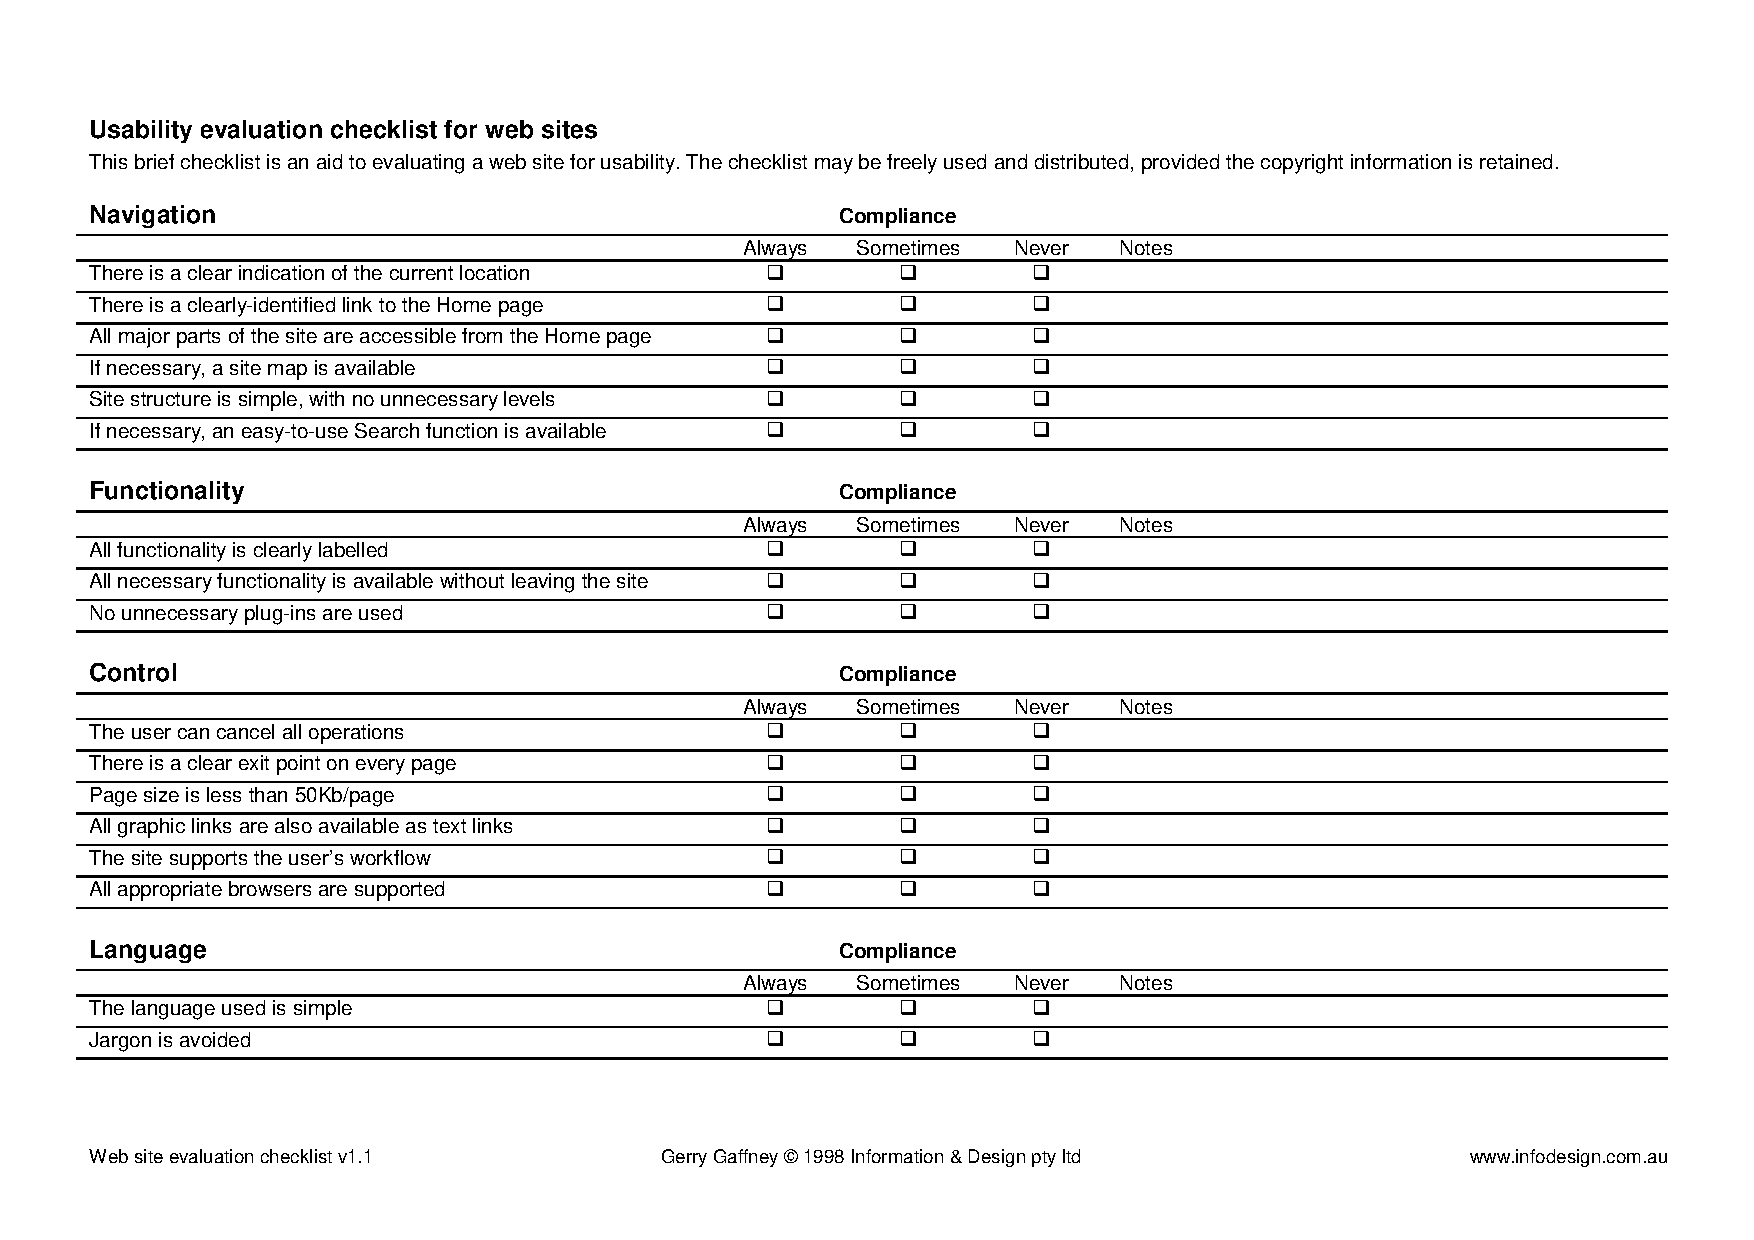
\includegraphics[page=1,width=1\textwidth]{pdf/apnd-webchecklist.pdf}
																																%\end{figure}
																																%\begin{figure}[H]
																																%	\centering\includegraphics[page=2,width=1\textwidth]{pdf/apnd-webchecklist.pdf}
																																%	\caption[Exemplo de uma \emph{Checklist}]{\label{apnd:checklist}Exemplo de uma lista de avaliação de usabilidade para websites (em inglês) -- Fonte: Information \& Design (1998). Disponível em: http://infodesign.com.au/wp-content/uploads/WebCheck.pdf}
																																%\end{figure}
																																
																																% E aqui (para a felicidade de todos) termina o documento.
																															\end{document}
